%; whizzy paragraph
%; whizzy-paragraph "^\\\\dancersection"
% -initex iniptex -latex platex -format platex -bibtex jbibtex -fmt fmt
% 以上 whizzytex を使用する場合の設定。

%     Tokyo Debian Meeting resources
%     Kansai Debian Meeting resources
%     Copyright (C) 2008 Junichi Uekawa
%     Copyright (C) 2008 Nobuhiro Iwamatsu

%     This program is free software; you can redistribute it and/or modify
%     it under the terms of the GNU General Public License as published by
%     the Free Software Foundation; either version 2 of the License, or
%     (at your option) any later version.

%     This program is distributed in the hope that it will be useful,
%     but WITHOUT ANY WARRANTY; without even the implied warranty of
%     MERCHANTABILITY or FITNESS FOR A PARTICULAR PURPOSE.  See the
%     GNU General Public License for more details.

%     You should have received a copy of the GNU General Public License
%     along with this program; if not, write to the Free Software
%     Foundation, Inc., 51 Franklin St, Fifth Floor, Boston, MA  02110-1301 USA

%   Pdf作成手順
% dvipdfmx debianmeetingresume200606.dvi
%  preview (shell-command (concat "evince " (replace-regexp-in-string "tex$" "pdf"(buffer-file-name)) "&"))
% 画像ファイルを処理するためにはebbを利用してboundingboxを作成。
%(shell-command "cd image2007-fuyu; ebb *.png")


% progress memo: 
% 2008/06-11がマージ対象、関西は2008/06-11
% イベント等でない場合は理由を書くこと。
% 必要な変更点は FIXME で記録しています。

%%ここからヘッダ開始。

\documentclass[mingoth,a4paper]{jsarticle}
\usepackage{monthlyreport}
\usepackage[dvips]{xy} % for advi workaround. Bug #452044

% section の代わりの環境 -- 改訂する。
\renewcommand{\dancersection}[2]{%
\newpage
あんどきゅめんてっど でびあん 2008年冬号
%
% top line
\vspace{0.1mm}\\
{\color{dancerlightblue}\rule{\hsize}{2mm}}

%
% middle text
%
\begin{minipage}[t]{0.6\hsize}
\color{dancerdarkblue}
\vspace{1cm}
\section{#1}
\hfill{}#2\\
\end{minipage}
\begin{minipage}[t]{0.4\hsize}
\vspace{-2cm}
\hfill{}
\includegraphics[height=8cm]{image200502/openlogo-nd.eps}\\
\vspace{-5cm}
\end{minipage}
%
%
{\color{dancerdarkblue}\rule{0.74\hsize}{2mm}}
%
\vspace{2cm}
}


% section の代わりの環境
\newcommand{\debconfsection}[2]{%
\newpage
あんどきゅめんてっど でびあん 2008年冬号
%
% top line
\vspace{0.1mm}\\
\colorbox{dancerlightblue}{\hspace{\hsize}}
%
% middle text
%
\begin{minipage}[t]{0.7\hsize}
\color{dancerdarkblue}
\vspace{1cm}
\section{#1}
\hfill{}#2\\
\end{minipage}
\begin{minipage}[t]{0.3\hsize}
\vspace{-2cm}
\hfill{}
\includegraphics[height=5cm]{image200706/logo-banner-split1.png}\\
\vspace{-5cm}
\end{minipage}
%
%
%vspace{-2cm}\\
\colorbox{dancerdarkblue}{\hspace{\hsize}}
%
\vspace{2cm}
}

\begin{document}
\begin{titlepage}
\includegraphics[height=252mm]{image2008-fuyu/2008-winter.eps}
%\thispagestyle{empty}
\end{titlepage}

\newpage
\begin{minipage}[]{0.2\hsize}
 \definecolor{titleback}{gray}{0.9}
 \colorbox{dancerlightblue}{\rotatebox{90}{\fontsize{80}{80} 
{\gt \color{dancerdarkblue}デビアン勉強会} }}
\end{minipage}
\begin{minipage}[]{0.8\hsize}
\hrule
\vspace{1mm}
\hrule
\setcounter{tocdepth}{1}
{\small
 \tableofcontents}
\vspace{1mm}
\hrule
\vspace{3cm}

\end{minipage}

% FIXME: 本文を追加すること。
% Debianパッケージング関係を先にもってくる
\dancersection{2008年度 Debian 勉強会企画}{上川 純一}
\label{sec:2008plan}
\index{2008@2008年度計画} 

2007年12月に実施した35回Debian勉強会で、一年分の実施したい内容を出してみ
ました。そこで策定した計画は以下です。

\begin{enumerate}
 \item 新年会「気合を入れる」
 \item Open Source Conference Tokyo (3/1)
 \item データだけのパッケージを作成してみる、
       ライセンスの考え方
 \item バイナリ一つのパッケージを作成してみる
       バージョン管理ツールを使いDebianパッケージを管理する(git)
       アップストリームの扱い(svn/git/cvs)
 \item バイナリの分かれたパッケージの作成。
       バイナリの分け方の考え方、アップグレードなどの運用とか。
 \item パッケージ作成(dpatch/debhelperで作成するパッケージ)
       man の書き方(roff or docbook)
 \item パッケージ作成(kernel patch、kernel module)
       、Debconf発表練習
 \item Debconf アルゼンチン、共有ライブラリパッケージ作成

 \item Open Source Conference Tokyo/Fall、
       デーモン系のパッケージの作成、latex、 emacs-lisp、フォントパッケージ
 \item パッケージの cross-compile の方法、amd64 上で i386 のパッケージと
       か、OSC-Fall報告会、Debconf報告会
 \item 国際化 po-debconf / po化 / DDTP
 \item 忘年会
\end{enumerate}

% tokyoresume200806 / 41
\dancersection{パッケージ作成(debhelper、CDBS、dpatch、quiltを用いたパッケージ作成)}{小林儀匡}
\label{sec:dpatchdebhelper}
\index{cdbs}
\index{debhelper} 
\index{quilt} 
\index{dpatch}

\subsection{はじめに}

この文書では、
まずDebianパッケージのビルドの流れと\texttt{debian/rules}の各ターゲットの役割を概観した上で、
debhelperやCDBSを用いて\texttt{debian/rules}をメンテナンスしやすくする方法を説明します。
次に、開発元のソースコードに対する変更をメンテナンスしやすいかたちで加える方法として、
パッチ管理ツールであるdpatchとquiltの使い方を説明します。

一般的なDebianパッケージの作成方法に興味のある読者を対象としています。

\subsection{前回までのおさらい}

これまでにパッケージの作成について学んだことを整理してみましょう。
簡単にまとめてしまえば、以下のようになるのではないでしょうか。

\begin{itemize}
 \item debパッケージの作成には、ソースツリーに\texttt{debian/changelog}、\texttt{debian/control}、\texttt{debian/copyright}、\texttt{debian/rules}という4つのファイルが最低限必要。
\begin{description}
 \item[debian/changelog] ソースファイルの変更履歴。
    最初のエントリが現在のバージョンに関する記述となり、
    ビルドされるパッケージのバージョン情報もここから抽出される。
 \item[debian/copyright] 著作権・ライセンス情報を収めたファイル。
    バイナリパッケージの\texttt{/usr/share/doc/$<$バイナリパッケージ名$>$/copyright}にインストールされる。
    現在のところ、debianディレクトリにありながら機械的に処理されることのない珍しいファイルで、
    書式も厳格には決められていない\footnote{書式を定めて機械可読にする議論がなされている。
    機械可読になった場合は、パッケージマネージャでライセンス情報を扱えるようになると考えられる。
    詳しくは\url{http://wiki.debian.org/Proposals/CopyrightFormat}を参照のこと。}。
 \item[debian/rules] ビルド方法を記述したGNU Make makefile。
 \item[debian/control] パッケージ (ソースパッケージおよびバイナリパッケージ) のメタ情報を指定するファイル。
    バージョン番号や作成日時など、バージョンごとに異なる情報はdebian/changelogに書かれるため、
    debian/controlには変更頻度の比較的低いメタ情報のみが収められる。
    また、生成されるソースパッケージとすべてのバイナリパッケージの名前もここで指定される。
    ファイルは空行で複数の段落に区切られており、
    そのうち最初の段落がソースパッケージおよびすべてのバイナリパッケージ用、
    その後に続く1つ以上の段落が各バイナリパッケージ用である。
\end{description} 
 \item \texttt{dh\_make}を使うと、これらのファイルや、
  ビルドに用いられるその他の設定ファイルの雛形を作成してくれる。
  それらを適当に編集してdebuildを実行するとソースパッケージおよびバイナリパッケージを作成できる。
\end{itemize}

一通りのパッケージ作成の流れや、
\texttt{debian/rules}以外のファイルの内容は何となく分かったかと思います。
しかし、debhelperのコマンドが連ねられている\texttt{debian/rules}については、
実際のところどのようなことをしており、
どのような流れでパッケージが作られているのかは、おそらくまだ理解できていないと思います。
また、パッケージをさらに細かく設定し、より洗練されたものにする方法も分からないでしょう。

そこで、今回は、\texttt{debian/rules}とdebhelperの各コマンドの内容を説明し、
パッケージがどのような過程を経てビルドされているのかを明らかにします。
その上で、debhelperやCDBSを用いて、
Debian Policy Manual (\emph{debian-policy})に準拠したパッケージをメンテナンスしやすいかたちで作成する方法を説明します。
また、開発元のソースコードに対する変更をメンテナンスしやすいかたちで加える方法として、
パッチ管理ツールであるdpatchとquiltの使い方を説明します。

まずビルドの流れについて見ていくことから始めましょう。

% ソースパッケージの構成とソースツリーについても語るべき?

% debian-policyに準拠したDebianパッケージとしてはもちろん必要だが、
% debian/changelogは現段階ではパッケージのビルド自体には不要?

\subsection{debパッケージのビルド手順}

debuildなどのパッケージビルドツールでは、大まかに言うと、
一般的に次のような手順でパッケージをビルドします。

\begin{enumerate}
 \item ビルド環境を整備する。
 \item 不要なファイルを削除する (\texttt{debian/rules clean})。
 \item ソースパッケージをまとめる (\texttt{dpkg-source -b $<$ディレクトリ名$>$})。
 \item バイナリパッケージにインストールするファイルをビルドする (\texttt{debian/rules build})。
 \item ビルドしたファイルをバイナリパッケージにまとめる (\texttt{debian/rules binary})。
 \item .changesファイルを作成する (\texttt{dpkg-genchanges})。
 \item パッケージに署名する。
\end{enumerate}

以下でこれらを詳しく説明します。

\subsubsection{ビルド環境を整備する}

実際にビルドを始める前に、まずはビルドのための環境を整える必要があります。

「ビルドのための環境を整える」と一口に言っても色々とありますが、
例えばソースパッケージの展開などが挙げられます。
ソースパッケージをビルドする場合は、
ソースパッケージを展開してソースツリーの状態にするところから始めなければなりません。
もちろんソースツリーでビルドする場合はこれは不要です。

また、
パッケージのビルドには、通常、様々なもの (コンパイラやライブラリなど) が必要となるので、
ビルド中にエラーにならないよう、それらの存在を確認しておく必要もあります。
必要となるパッケージは、ソースパッケージの場合は\texttt{.dsc}ファイルのBuild-Dependsフィールド、
ソースツリーの場合はdebian/controlのBuild-Dependsフィールドに書かれています。
ビルドツールによっては、ビルドに必要なパッケージを確認するだけでなく、
インストールされていない場合にインストールしてくれるものもあります。

また、pdebuildなどのようにchroot環境内でパッケージをビルドするツールは、
こういった作業の前にまずchroot環境を作ってそこに入るところから始めるでしょう。

\subsubsection{不要なファイルを削除する (\texttt{debian/rules clean})}

必要なパッケージが揃っていることを確認したところで、
不要なファイルを削除します。
一般に、以前のビルドで生成されたファイルがある場合はそれを削除して、
常に同じ状態からビルドできるようにすべきです。
\texttt{debian/rules}のcleanターゲットをそのような目的で使うよう、
debian-policyにおいて定められています。

\subsubsection{ソースパッケージをまとめる (\texttt{dpkg-source -b $<$ディレクトリ名$>$})}

ソースパッケージを作成するタイミングとしては、不要なファイルを削除した後、
バイナリパッケージに含めるファイルのビルドに入る前が最もよいでしょう。
\texttt{dpkg-source}コマンドの\texttt{-b}オプションを使うと、
ソースツリーからソースパッケージを作成できます。

\subsubsection{バイナリパッケージにインストールするファイルをビルドする (\texttt{debian/rules build})}

ソースパッケージを作成し終えたらいよいよバイナリパッケージの作成に移ります。
バイナリパッケージの作成は大きく2段階に分けることができます。
最初の段階は、設定やコンパイルです。

Cなどの言語で書かれたプログラムやライブラリがパッケージに含まれている場合、
それらをインストール前にコンパイルして、
バイナリのプログラムやライブラリを作成する必要があります。
プログラムのビルドにGNU Autoconfを使用するようになっている場合は、
コンパイルの前にconfigureスクリプトを走らせて設定を行う必要もあるでしょう。

この手続きは、
バイナリのプログラムやライブラリを含んでいないパッケージについても必要になることが多いでしょう。
例えば、\LaTeX{}やSGMLなどの形式で書かれたドキュメントは、
HTMLやPostScript、PDFなどの配布に適した形式に変換してバイナリパッケージに含めるべきです。
また、ソースとなるデータを変換してインストール用のデータを作成する必要がある場合も、
通常はここでその変換を行います。

debian-policyでは、
このような、プログラムやライブラリの設定・コンパイルやデータの変換のために、
\texttt{debian/rules}のbuildターゲットを使うよう指定されています。

% tarballからソフトウェアのインストールをしたことがあるかたは、
% 「./configure; make」のプロセスと言えばお分かりかと思います。

\subsubsection{ビルドしたファイルをバイナリパッケージにまとめる (\texttt{debian/rules binary})}

必要なファイルをすべてビルドしたところで、
それらを適切なパーミッションで適切な場所に配置し、
バイナリパッケージにまとめ上げる必要があります。
あっさりと書いてしまいましたが、
debian-policyに準拠するパッケージを手で作成しようとする場合には、
かなり複雑で面倒な作業を要求されるプロセスです。

このプロセスは、通常、
まずdebian/tmpを/と見なしてソフトウェア全体のインストール (「仮インストール」) を行い、
その上でdebian/tmp内の各ファイルを適切にdebian/$<$バイナリパッケージ名$>$に振り分け、
最後にdebian/$<$バイナリパッケージ名$>$をそれぞれバイナリパッケージ化する、
という流れで行います。
debian/$<$バイナリパッケージ名$>$をバイナリパッケージ化する際には、
パーミッションの調節やファイルの圧縮など、
しなければならないこと、推奨されていることが多数あります。
それらは後で詳述しますので、ここでは詳しい説明は省きます。

debian-policyでは、バイナリパッケージをまとめ上げるために、
\texttt{debian/rules}のbinaryターゲットを使うよう指定されています。

\subsubsection{.changesファイルを作成する (\texttt{dpkg-genchanges})}

ソースパッケージとバイナリパッケージのファイルが一通り揃ったところで、
これらのファイルに関する情報をまとめた\texttt{.changes}ファイルを作成する必要があります。
これには\texttt{dpkg-genchanges}コマンドが使用されます。

\subsubsection{パッケージに署名する}

私家版パッケージやテストビルドでは必要ありませんが、公式パッケージにする場合は、
最後にパッケージに署名する必要があります。
公式パッケージにしない場合でも、広く配布する場合には署名することをお勧めします。

署名は、\texttt{.dsc}ファイルと\texttt{.changes}ファイルに対して行います。
\texttt{.dsc}ファイルにはソースパッケージの\texttt{.tar.gz}ファイルと\texttt{.diff.gz}ファイルのハッシュとサイズが書かれているので、
署名を施すことでこれらのファイルの品質を保証できます。
また、\texttt{.changes}ファイルにはソースパッケージとバイナリパッケージのすべてのファイルのハッシュとサイズが書かれているので、
署名を施すことでこれらのファイルすべての品質を保証できます\footnote{厳密に言えば、
以前のバージョンと同一の\texttt{.tar.gz}ファイルを使用している場合は、
\texttt{.tar.gz}ファイルの情報は\texttt{.changes}ファイルには記載されません。
したがって、この場合は\texttt{.dsc}ファイルを経由した間接的な保証となります。}。

署名には、通常、devscriptsパッケージに含まれているdebsignコマンドを使います。
このコマンドは、最初に\texttt{.dsc}ファイルに対する署名を行い、その後で、
\texttt{.changes}内の\texttt{.dsc}ファイルのエントリのハッシュやサイズを署名後の値に置換した上で、
\texttt{.changes}ファイルに署名してくれます。

\subsection{debian/rulesのターゲット}

ビルド手順の説明から分かるかと思いますが、
\texttt{debian/rules}には、パッケージのビルド時に必要となるターゲットがあります。
説明に登場したclean、build、binaryの他に、binary-archとbinary-indepも必須のターゲットです。
以下でこれらのターゲットの役割を簡単に示します (詳細はdebian-policyを参照してください)。

\begin{description}
 \item[clean]
    buildターゲットやbinaryターゲットで行った変更をすべて元に戻すためのターゲットです。
    ただし、生成されたバイナリパッケージの削除はすべきでありません。
    このターゲットはroot権限で呼び出す必要があるかもしれません。
 \item[build]
    バイナリパッケージに含めるプログラムやライブラリの設定・コンパイルやデータの変換に使用されるターゲットです。
    設定が対話的だとパッケージの自動ビルドができなくなるため、
    設定は非対話的なものでなければなりません。
    インストールパスなどの設定を対話的に行うようになっているソフトウェアについては、
    設定用のプログラムの書き換えなどで対応してください。
    このターゲットでは、root権限が必要な操作を行ってはなりません。
 \item[binary]
    binaryターゲットは、
    buildターゲットでビルドされたバイナリパッケージをまとめ上げるのに使用されます。
    binaryターゲットは、通常、
    binary-archターゲットとbinary-indepターゲットに依存するだけとなります。
    このターゲットはroot権限で呼び出されなくてはなりません。
 \item[binary-arch]
    ビルドされたファイルから特定アーキテクチャ用バイナリパッケージを生成するためのターゲットです。
    パッケージに含めるファイルをビルドするターゲットとして、
    buildターゲット (または定義されている場合はbuild-archターゲット) に依存するようにしておくべきです。
    このターゲットはroot権限で呼び出されなくてはなりません。
 \item[binary-indep]
    ビルドされたファイルからアーキテクチャ非依存バイナリパッケージを生成するためのターゲットです。
    パッケージに含めるファイルをビルドするターゲットとして、
    buildターゲット (または定義されている場合はbuild-indepターゲット) に依存するようにしておくべきです。
    このターゲットはroot権限で呼び出されなくてはなりません。
\end{description}

clean、build、binaryについては、
パッケージのトップレベルディレクトリ (debianディレクトリの親ディレクトリ) をカレントディレクトリとして実行するよう定められています。

\subsection{debhelperを使わないdebian/rules}

\texttt{debian/rules}の必須ターゲットに関する規約を簡単に眺めたところで、
実際のパッケージの\texttt{debian/rules}の例を見てみましょう。
以下では、Debianパッケージ作成用のツールを何も使わずに実装した、
helloパッケージの\texttt{debian/rules}から抽出したコード (を一部改変したもの) を例に示します。

まずはcleanターゲットです。

\begin{commandline}
clean:
	rm -f build
	-$(MAKE) -i distclean
	rm -rf *~ debian/tmp debian/*~ debian/files* debian/substvars
\end{commandline}

簡単に読めますね。
以下のことをやっているだけです。

\begin{itemize}
 \item タイムスタンプとして使用したbuildファイルを削除する。
 \item ソフトウェアのMakefileのdistcleanターゲットを実行し、
  ソフトウェアのビルドで生成されたファイルを削除する。
 \item パッケージのビルド時にdebianディレクトリ内に作成されたファイルを削除する。
\end{itemize}

続いてbuildターゲットです。

\begin{commandline}
CC = gcc
CFLAGS = -g -Wall

ifeq (,$(findstring noopt,$(DEB_BUILD_OPTIONS)))
  CFLAGS += -O2
endif

build:
	./configure --prefix=/usr
	$(MAKE) CC="$(CC)" CFLAGS="$(CFLAGS)"
	touch build
\end{commandline}

GNU Makeのmakefileに慣れていないと、変数の設定の部分が分かりにくいかもしれませんが、
buildターゲット自体は非常に単純ですね。
ソフトウェアをソースからインストールしたことのあるかたならお馴染みの、
Autoconfを用いた一般的なCプログラムのビルド方法です。

最後に、binary、binary-arch、binary-indepの3つのターゲットです。

\begin{commandline}
package = hello
docdir = debian/tmp/usr/share/doc/$(package)

INSTALL_PROGRAM = install

ifeq (,$(findstring nostrip,$(DEB_BUILD_OPTIONS)))
  INSTALL_PROGRAM += -s
endif

binary-indep: build

binary-arch: build
	rm -rf debian/tmp
	install -d debian/tmp/DEBIAN $(docdir)
	$(MAKE) INSTALL_PROGRAM="$(INSTALL_PROGRAM)" \
		prefix=$(CURDIR)/debian/tmp/usr install
	cp -a NEWS debian/copyright $(docdir)
	cp -a debian/changelog $(docdir)/changelog.Debian
	cp -a ChangeLog $(docdir)/changelog
	cd $(docdir) && gzip -9 changelog changelog.Debian
	gzip -r9 debian/tmp/usr/share/man
	dpkg-shlibdeps debian/tmp/usr/bin/hello
	dpkg-gencontrol
	chown -R root:root debian/tmp
	chmod -R u+w,go=rX debian/tmp
	dpkg-deb --build debian/tmp ..

binary: binary-indep binary-arch
\end{commandline}

一つずつ手順を追っていけば、
以下のような手順でバイナリパッケージを生成していることが分かります。

\begin{enumerate}
 \item インストール先のディレクトリを準備する。
 \item ソフトウェアのMakefileのinstallターゲットで、
    インストール先のディレクトリにファイルをインストールする。
    環境変数\texttt{DEB\_BUILD\_OPTIONS}にnostripという文字が含まれていない場合は、
    インストール時に、オブジェクトファイルからシンボルを切り捨てる (stripする)。
 \item インストール先のドキュメント用ディレクトリに、
    ソフトウェアのドキュメントやdebian/copyrightをインストールする。
 \item インストール先のドキュメント用ディレクトリに、
    debian/changelogおよびソフトウェアのChangeLogを、
    それぞれchangelog.Debianおよびchangelogとしてインストールする。
 \item インストールしたchangelog.Debianおよびchangelogやマニュアルページを圧縮する。
 \item インストールしたバイナリファイルの、ビルドに使われたライブラリへの依存関係を調べて、
    debian/substvarsに変数\$\{shlibs:Depends\}を設定する。
 \item debian/controlを元にdebian/tmp/DEBIAN/controlを作成する。
    その際に、debian/control内の「\$\{shlibs:Depends\}」を、
    先に設定した変数の値で置換する。
 \item インストール先のディレクトリやファイルのパーミッションを適切に設定する。
 \item debパッケージにする。
\end{enumerate}

バイナリプログラム1つと付随データをバイナリパッケージ1つにインストールするだけなのに、
かなり複雑な手順を踏んでいます。
これは以下のような理由からです。

\begin{itemize}
 \item 以下のようなものに関してdebian-policyの規約に従う必要がある。
\begin{itemize}
 \item インストールすべきドキュメント
 \item インストールされたファイルのパーミッション
 \item 圧縮すべきファイル
 \item オブジェクトファイル内のシンボルの扱い
\end{itemize} 
 \item 依存関係の記述を簡単にするための変数「\$\{shlibs:Depends\}」を処理する必要がある。
 \item debian/tmp/DEBIAN以下に、debian/controlなどのパッケージのメタ情報を含むファイルや、
  メンテナスクリプトを入れなければならない。
\end{itemize}

バイナリパッケージ1つを生成するパッケージでさえこれだけの手順を踏まなければならないので、
様々なファイルを複数のバイナリパッケージに分けてインストールするようなパッケージの作成に、
かなり手間がかかるのは容易に想像できます。

\begin{screen}
\paragraph*{debファイルの内容}

dpkg-deb --buildがどのようにして複数のファイルを1つの「パッケージ」にまとめているか、
興味があるかもしれません。
そのような場合は、以下の実行例が参考になるでしょう。

\begin{commandline}
noritada[3:50]%  ls                       
hello_2.2-2_i386.deb
noritada[3:50]%  ar x hello_2.2-2_i386.deb
noritada[3:50]%  ls 
control.tar.gz	data.tar.gz  debian-binary  hello_2.2-2_i386.deb
noritada[3:50]%  cat debian-binary 
2.0
noritada[3:50]%  tar ztf control.tar.gz 
./
./control
noritada[3:50]%  tar ztf data.tar.gz 
./
./usr/
./usr/share/
./usr/share/doc/
./usr/share/doc/hello/
[snip]
./usr/share/man/
./usr/share/man/man1/
./usr/share/man/man1/hello.1.gz
./usr/bin/
./usr/bin/hello
\end{commandline}
\end{screen}

\subsection{debhelperを用いたdebian/rules}

debian-policyの規約に従ったDebianパッケージを容易に作成できるようにしてくれるのが、
debhelperです。
例として、先程のhelloパッケージに対してdebhelperを使用したhello-debhelperパッケージの\texttt{debian/rules}を見てみましょう。

まずはcleanターゲットです。

\begin{commandline}
clean:
	dh_clean
	rm -f build
	-$(MAKE) -i distclean
\end{commandline}

helloパッケージの場合とほぼ同じですが、
debianディレクトリの掃除に関しては\texttt{dh\_clean}というコマンドを使用していることが分かります。

次はbuildターゲットですが、これはhelloパッケージのものとまったく同じなので省略します。

最後に、helloパッケージではかなり複雑だった、
binary、binary-arch、binary-indepの3つのターゲットです。

\begin{commandline}
package = hello-debhelper

install: build
	dh_clean
	dh_installdirs
	$(MAKE) prefix=$(CURDIR)/debian/$(package)/usr install

binary-indep: install

binary-arch: install
	dh_installdocs -a NEWS
	dh_installchangelogs -a ChangeLog
	dh_strip -a
	dh_compress -a
	dh_fixperms -a
	dh_installdeb -a
	dh_shlibdeps -a
	dh_gencontrol -a
	dh_md5sums -a
	dh_builddeb -a

binary: binary-indep binary-arch
\end{commandline}

「dh\_」で始まるコマンド群で占められているのが分かります。
これらがdebhelperのコマンドです。
オプションやファイル名の指定などは部分的にはあるものの、
基本的には非常にシンプルな記述となっており、
バイナリパッケージ名やインストールパスなどの具体的な情報を記述する必要がなくなっています。
ここでは単一のバイナリパッケージの例を取り上げていますが、
複数のバイナリパッケージを生成する\texttt{debian/rules}についても同様にシンプルに記述できます。
それは、debhelperの、以下のような特長からです。

\begin{itemize}
 \item インストールされたデータをdebian-policyの規約に従うように修正するコマンドを持つ。
\begin{itemize}
 \item \texttt{dh\_strip}: オブジェクトファイル内のシンボルの切り捨て
 \item \texttt{dh\_compress}: テキストファイルの圧縮
 \item \texttt{dh\_fixperms}: パーミッションの修正
\end{itemize} 
\item デフォルトで、
  バイナリパッケージのインストールパスをdebian/$<$バイナリパッケージ名$>$と仮定して動作する\footnote{ちなみに、上のコードで様々なコマンドについている「-a」は、
  「アーキテクチャ依存バイナリパッケージすべてに適用する」という意味です。}。
 \item デフォルトですべてのバイナリパッケージに対して動作する。
 \item debパッケージ作成に必要となるdpkgのコマンドをうまくラップして、
  他のdebhelperのコマンドと同じようなかたちで実行できるようにする。
\end{itemize}

debhelperは、\texttt{debian/rules}をメンテナンスする手間を大きく減らしてくれる、
非常に有用なツールだと言えます。

% dh_makeで作成したdebhelper式debian/rulesだと、
% dh_testdirやdh_testrootが目立つので、
% これらも追加しておいたほうがよい??

% helloパッケージのほうではdh_md5sumsに対応する操作をしていないので、
% 追加したほうがよい??

\subsection{debhelperのコマンド群}

debhelperの特長を説明したところで、そのコマンド群を概観しましょう。
と言っても、コマンドの役割やオプションの説明、必要となる設定ファイルについては、
各コマンドのマニュアルページや書籍『[入門] Debianパッケージ』に詳しい記述があるので、
それらに譲ります。
ここでは、大まかな分類と使い方の説明に焦点を絞った話をします。

\texttt{debian/rules}の記述を減らしてくれるdebhelperですが、
「多数のコマンドのどれをどのタイミングで使うべきか分かりにくい」という欠点があります。
それは、上で述べたように、debian-policyの規約やdpkgのコマンドごとに、
debhelperにも対応するコマンドが存在するため、
debhelperを使用しても、debパッケージにまとめるまでの手順は多いからです。
そこで、ここでは、使用する状況によってコマンドを7つに分類しておきます。
debhelperで\texttt{debian/rules}を書く際の参考にしていただけると幸いです。

なお、「binary系ターゲット」とは、
binary、binary-arch、binary-indepの3つのターゲットのことです。

\subsubsection{確認系}

以下のコマンドは、各ターゲットの頭において、
ターゲットを正しい条件で実行しようとしているか確認するために使われるものです。

\begin{itemize}
 \item \texttt{dh\_testroot}
 \item \texttt{dh\_testdir}
\end{itemize}

\subsubsection{掃除系}

以下のコマンドは、cleanターゲットで使われるものです。

\begin{itemize}
 \item \texttt{dh\_clean}
\end{itemize}

\subsubsection{インストール前処理系}

以下のコマンドは、binary系ターゲットにおいて、仮インストールの準備段階で実行すべきものです。

\begin{itemize}
 \item \texttt{dh\_clean}
 \item \texttt{dh\_installdirs}
\end{itemize}

\subsubsection{インストール系}

以下のコマンドは、binary系ターゲットにおいて、
仮インストール後にファイルなどをdebian/$<$バイナリパッケージ名$>$以下にインストールするのに使われます。

\begin{itemize}
 \item \texttt{dh\_install}
 \item \texttt{dh\_installcatalogs}
 \item \texttt{dh\_installchangelogs}
 \item \texttt{dh\_installcron}
 \item \texttt{dh\_installdebconf}
 \item \texttt{dh\_installdocs}
 \item \texttt{dh\_installemacsen}
 \item \texttt{dh\_installexamples}
 \item \texttt{dh\_installinfo}
 \item \texttt{dh\_installinit}
 \item \texttt{dh\_installlogcheck}
 \item \texttt{dh\_installlogrotate}
 \item \texttt{dh\_installman}
 \item \texttt{dh\_installmenu}
 \item \texttt{dh\_installmime}
 \item \texttt{dh\_installpam}
 \item \texttt{dh\_installudev}
 \item \texttt{dh\_link}
 \item \texttt{dh\_lintian}
\end{itemize}

\subsubsection{後処理系}

以下のコマンドは、binary系ターゲットにおいて、
debian/$<$バイナリパッケージ名$>$以下にインストールされたファイルを、
debian-policyに適合するよう修正するのに使われます。

\begin{itemize}
 \item \texttt{dh\_compress}
 \item \texttt{dh\_fixperms}
 \item \texttt{dh\_strip}
\end{itemize}

\subsubsection{deb化準備系}

以下のコマンドは、binary系ターゲットにおいて、
debパッケージ生成の直前に行う処理に使用されます。

\begin{itemize}
 \item \texttt{dh\_installdeb}
 \item \texttt{dh\_perl}
 \item \texttt{dh\_shlibdeps}
\end{itemize}

\subsubsection{deb化系}

以下のコマンドは、binary系ターゲットにおいて、
debパッケージ生成の直前に行う処理に使用されます。

\begin{itemize}
 \item \texttt{dh\_gencontrol}
 \item \texttt{dh\_md5sums}
 \item \texttt{dh\_builddeb}
\end{itemize}

\subsection{debian/rulesをさらに簡潔に書くには}

debhelperの様々なコマンドを、使用するタイミングによって7つに分類してみました。
これによって浮かび上がってくるのは、
「どのパッケージでもコマンドを呼び出す順番はほぼ同じ」という事実です。
実際、\texttt{dh\_make}で作成した\texttt{debian/rules}の雛形をいじる場合でも、
debhelperコマンド群の呼び出し順序を変更することはほとんどないでしょう。

ここで、「ではコマンド群の呼び出しの流れを一般化してしまえば、debhelperのコマンドばかりが並んだ、似たような\texttt{debian/rules}を量産しないで済む」と気付くと思います。
実際問題として、雛形から作成した、似たような\texttt{debian/rules}を多数管理するのはコストがかかります。
新しいコマンドができた場合、それをすべての\texttt{debian/rules}の同じ場所に加えればなりません。

そこで登場するのがCDBSです。
次は、CDBSのdebhelperルールを用いて\texttt{debian/rules}をさらに簡潔にします。

\subsection{CDBSのdebhelperルールを用いたdebian/rules}

「似た内容の、短くはない\texttt{debian/rules}を量産する」というdebhelperの欠点を解決するのが、
CDBSのdebhelperルール (debhelper.mk) です。
CDBSとは、
\texttt{debian/rules}の記述をモジュール化して再利用できるようにしたものをライブラリとして提供し、
一般的な流れに沿った\texttt{debian/rules}を非常に簡単に記述できるようにするシステムです。
CDBSのdebhelperルール (debhelper.mk) では、
debhelperを用いたビルドの一般的な流れが既に定義されているので、
debhelperの各コマンドに与えるオプションや引数を指定するだけで\texttt{debian/rules}が書けます。

hello-debhelperの\texttt{debian/rules}をCDBSのdebhelperルールを用いて書き換えると、
次のようになります。

\begin{commandline}
#!/usr/bin/make -f

include /usr/share/cdbs/1/rules/debhelper.mk

package = hello-cdbs

CC = gcc
CFLAGS = -g -Wall

ifeq (,$(findstring noopt,$(DEB_BUILD_OPTIONS)))
  CFLAGS += -O2
endif

clean::
	-$(MAKE) -i distclean

install/hello-cdbs::
	$(MAKE) prefix=$(CURDIR)/debian/$(package)/usr install

common-configure-arch::
	./configure --prefix=/usr

common-build-arch::
	$(MAKE) CC="$(CC)" CFLAGS="$(CFLAGS)"

DEB_INSTALL_DOCS_ALL := NEWS
DEB_INSTALL_CHANGELOGS_ALL := ChangeLog
\end{commandline}

書き換えは、以下のような手順で行いました。

\begin{enumerate}
 \item \texttt{/usr/share/cdbs/1/rules/debhelper.mk}をインクルードする。
 \item debhelperのコマンドをすべて削除し、引数やオプションは変数に設定しなおす
 \item ターゲットの指定を通常のコロンから二重コロンに変更する。
 \item ターゲット名を書き換える。
\end{enumerate}

以下でこれらを詳しく説明します。

\subsubsection{\texttt{/usr/share/cdbs/1/rules/debhelper.mk}をインクルードする}

debhelperルールの定義を取り込むには、
\texttt{/usr/share/cdbs/1/rules/debhelper.mk}をインクルードする必要があります。

\subsubsection{debhelperのコマンドをすべて削除し、引数やオプションは変数に設定しなおす}

debhelperのコマンドは、引数やオプションがついていないものについては削除してかまいません。
対応する操作がdebhelperルール内で定義されています。

引数やオプションがついている場合は、その内容を変数に設定しなおす必要があります。
CDBSのdebhelperルールでは、
debhelperの各コマンドの引数やオプションに対応する変数を使用するようになっています。
変数の例を示します。

\begin{description}
 \item[\texttt{DEB\_INSTALL\_DOCS\_$<$バイナリパッケージ名$>$}]
    $<$バイナリパッケージ名$>$にインストールしたいドキュメントのリストを設定します。
    値が設定されると、適切なタイミングで、
    「\texttt{dh\_installdocs -p $<$バイナリパッケージ名$>$ $<$変数の値$>$}」が実行されます。
 \item[\texttt{DEB\_INSTALL\_DOCS\_ALL}]
    すべてのバイナリパッケージにインストールしたいドキュメントのリストを設定します。
    値が設定されると、適切なタイミングで、
    「\texttt{dh\_installdocs -A $<$変数の値$>$}」が実行されます。
\end{description}

\subsubsection{ターゲットの指定を通常のコロンから二重コロンに変更する}

CDBSを使用する場合は、ターゲットの指定に二重コロンを使用する必要があります。
これは、モジュール化に、
「ターゲットを二重コロンで指定することで処理を多重定義できる」というGNU Make makefileの機能を使用していためです。
以下のリストのように、通常のコロンの場合は後で指定された処理が実行されますが、
二重コロンで定義すると両方の処理が実行されます。

\begin{commandline}
noritada[10:22]%  cat Makefile 
hoge:
        @echo foo

hoge:
	@echo bar
noritada[10:22]%  make
Makefile:5: 警告: ターゲット `hoge' へのコマンドを置き換えます
Makefile:2: 警告: ターゲット `hoge' への古いコマンドは無視されます
bar
noritada[10:22]%  cat Makefile 
hoge::
	@echo foo

hoge::
	@echo bar
noritada[10:22]%  make
foo
bar
\end{commandline}

\subsubsection{ターゲット名を書き換える}

CDBSのdebhelperルール\footnote{厳密に言えばdebhelperルールがインクルードしているbuildcoreルール。}では、
binaryやbuild-arch、build-indepなどの大きな流れを表すターゲットを複数の処理に分割し、
ユーザが処理の多重定義を用いて適切なタイミングで処理を挿入できるようにしています。
ターゲットの例を示します。

\begin{description}
 \item[common-configure-arch]
    configureスクリプトのようなものを用いてビルド前にパッケージを設定するのに使用されます。
    これはアーキテクチャ依存のバイナリパッケージに対するものです。
 \item[common-configure-indep]
    configureスクリプトのようなものを用いてビルド前にパッケージを設定するのに使用されます。
    これはアーキテクチャ非依存のバイナリパッケージに対するものです。
 \item[common-build-arch]
    Makefileのallターゲットのようなものを用いてソフトウェアをビルドするのに使用されます。
 \item[install/$<$バイナリパッケージ名$>$]
    Makefileのinstallターゲットのようなものを用いて仮インストールを行うのに使用されます。
\end{description}

\subsection{ここまでのまとめ}

パッケージのビルド方法や\texttt{debian/rules}の各ターゲットの役割を概観した上で、
\texttt{debian/rules}をより簡潔に、より分かりやすく書く方法を求めて、
debhelperやCDBSを見てきました。
簡潔に分かりやすく書くことはメンテナンスのしやすさに繋がるので、
できるだけ\texttt{debian/rules}をシンプルに保つことをお勧めします。

\subsection{パッチ管理ツールを用いた開発元のソースコードの修正}

これまではdebianディレクトリ以下のみをいじってきましたが、
最後に、開発元が配布しているソースコードに修正を加える方法を説明します。
\texttt{debian/rules}についてはメンテナンスのしやすさを重要視しましたが、
それは、開発元が配布しているソースコードに修正を加える際にも当てはまります。

Debianパッケージを管理していると、開発元のソースコードに手を加えたくなることがよくあります。
理由は様々です。

\begin{itemize}
 \item 解決したい問題が、次期リリースに向けて開発中のソースコードでは既に修正されているのだが、
  次期リリースは暫く出そうにもない。
  パッケージについては一足早く修正しておきたい。
 \item 開発元で開発がなされなくなったため、ソフトウェアの問題を自分で解決する必要がある。
\end{itemize}

こんなときに、開発元のソースコードに修正を加える最も簡単な方法は、
debianディレクトリの外側のソースコードを直接いじることです。
ネイティブでないDebianソースパッケージは、
\texttt{.tar.gz}ファイルと\texttt{.diff.gz}ファイル、\texttt{.dsc}ファイルから成るので、
ソースコードに変更を加えれば、
それは開発元のソースコードからの差分として \texttt{.diff.gz}ファイルに含まれます。

しかし、この安直な方法にはもちろん大きな問題があります。

\begin{itemize}
 \item 時間が経つと加えた変更の背景や目的が分からなくなる。
 \item 変更の数が増えていくと混ざってしまい、意味的なまとまりのある単位で変更を切り分けにくくなる。
 \item 開発元から新しいバージョンがリリースされたときに、
  そのバージョンでも有効な変更とそのバージョンでは無効な変更を切り分けられなくなる。
\end{itemize}

そこで、変更を開発元のソースコードに直接加えることはせず、dpatchやquiltを用いて、
意味的なまとまりのある単位でパッチとして管理することが推奨されています。
簡単にまとめると、以下のような方法です。

\begin{itemize}
 \item 変更はすべてパッチとしてdebianディレクトリ以下に保持しておき、
  開発元のソースコードには直接的な改変は一切加えない。
 \item パッケージのビルド時には当てたり外したりする。
  ソースパッケージをビルドするときには外した状態にしておき、
  バイナリパッケージをビルドするときには当てた状態にしておく。
 \item パッケージの更新時には、各パッチについて、有効性を吟味する。
\end{itemize}

ここでは、簡単にその使い方を見ていきます。

\subsubsection{パッチ置き場}

一般に、dpatchやquiltでパッチを管理する場合は、
debian/patchesディレクトリをパッチ置き場として使用します。
dpatchの場合はdebian/patches/00listが、
quiltの場合はdebian/patches/seriesがそれぞれパッチのリストとなっており、
debian/patchesに含まれている一連のパッチが、
このパッチリストに記載されている順に適用されていきます。

dpatchを使用しているkazehakaseパッケージのdebian/patchesの例:

\begin{commandline}
noritada[16:39]%  ls debian/patches/*
debian/patches/00list
debian/patches/05_add_missing.dpatch
debian/patches/20_user_agent_tag.dpatch
debian/patches/30_bookmarkbar_DSA.dpatch
debian/patches/50_passwordmgr.dpatch
debian/patches/60_fix_ftbfs.dpatch
debian/patches/70_enable_gtk_deprecated.dpatch
debian/patches/80_NSIBADCERTLISTNER.dpatch
noritada[16:39]%  cat debian/patches/00list
20_user_agent_tag
30_bookmarkbar_DSA
50_passwordmgr
\end{commandline}

quiltを使用しているskksearchパッケージのdebian/patchesの例:

\begin{commandline}
noritada[16:52]%  ls debian/patches/*
debian/patches/clean-build-errors-and-warnings.diff
debian/patches/conf-file.diff
debian/patches/db4.3.diff
debian/patches/dic-bufsize.diff
debian/patches/plain-search.diff
debian/patches/series
noritada[16:52]%  cat debian/patches/series
conf-file.diff
db4.3.diff
dic-bufsize.diff
plain-search.diff
clean-build-errors-and-warnings.diff
\end{commandline}

\subsubsection{パッチ管理}

パッチを当てるには、
dpatchの場合はdpatch applyを、quiltの場合はquilt pushを使用してください。
外すには、dpatchの場合はdpatch deapplyを、quiltの場合はquilt popを使用してください。

新たなパッチを作成するには、まずパッチをどこに挟むか決めてください。
dpatchにおいて$<$あるパッチ$>$の次に挟む場合は、次のように行います。

\begin{commandline}
$ dpatch-edit-patch patch <新規パッチ> <あるパッチ>
$ editor <あるファイル> (パッチに含める変更を加えます)
$ exit 0
\end{commandline}

quiltにおいて同様の操作を行う場合は、次のようにします。

\begin{commandline}
$ quilt push <あるパッチ> (<あるパッチ>が既に当たっている場合は、quilt pop <あるパッチ>になります)
$ quilt new <新規パッチ>
$ quilt add <あるファイル> (パッチの作成を開始した後、変更する対象はaddで追加しておく必要があります)
$ editor <あるファイル> (パッチに含める変更を加えます)
$ quilt refresh
\end{commandline}

変更を加えるためにエディタを使う場合は、
「\texttt{quilt edit $<$あるファイル$>$}」を実行すれば、
「\texttt{quilt add $<$あるファイル$>$}」を実行せずに編集することも可能です。

\subsubsection{ビルド時に適切にパッチを取り扱う}

折角パッチをdebian/patchesに入れておいたところで、
ソースパッケージをビルドするときにはパッチを外した状態にしておき、
バイナリパッケージをビルドするときにはパッチを当てた状態にしておかなければ、
意味がありません。
これは、\texttt{debian/rules}でパッチに関する依存関係を適切に設定することで実現できます。
以下では、様々な場合について、\texttt{debian/rules}の記述例を示します。

まず、dpatchについてです。
debhelperを使用している場合は、\\
\texttt{/usr/share/doc/dpatch/examples/rules/rules.new.dh.gz}を参考にしてください。

\begin{commandline}
build: build-stamp
build-stamp: patch
	dh_testdir
	# ここでソフトウェアをビルドする。
	touch build-stamp

clean: clean1 unpatch
clean1:
	dh_testdir
	dh_testroot
	dh_clean -k
	# ここで掃除をする。

patch: patch-stamp
patch-stamp:
	dpatch apply-all
	dpatch cat-all >patch-stamp
	touch patch-stamp

unpatch:
	dpatch deapply-all
	rm -rf patch-stamp debian/patched
\end{commandline}

CDBSを利用している場合は、CDBSのドキュメントにあるとおり、
以下のような行を加えるだけでかまいません。
ただし、autotools.mkをインクルードしている場合は、
dpatch.mkをインクルードするのはそれよりも後ろにしてください。

\begin{commandline}
include /usr/share/cdbs/1/rules/dpatch.mk
\end{commandline}

quiltについても、
CDBSを利用している場合は、CDBSのドキュメントにあるとおり、
以下のような行を加えるだけでかまいません。

\begin{commandline}
include /usr/share/cdbs/1/rules/patchsys-quilt.mk
\end{commandline}

\begin{screen}
\paragraph*{パッチ管理ツールの近況と今後}

Debianで長いこと使われてきたパッチ管理ツールdpatchについては、
\texttt{dh\_make}が、1ヶ月ほど前にバージョン0.45で\texttt{--dpatch}オプションを提供し始めました。
これまでは、パッケージ化への入口となる\texttt{dh\_make}によるサポートがなかったため、
「パッチ管理ツールはパッケージメンテナが好みで使用するもの」という雰囲気があったように思いますが、
今後、パッチ管理が普及し、開発元のソースコードは一切いじらないという風潮が強くなるのだとしたら、
嬉しいことです。

一方でquiltについては、昔は非常にマイナーなパッチ管理ツールでしたが、
xorgを管理するDebian X Strike Forceやglibcを管理するDebian GNU Libc Maintainersなど、
大規模なパッケージで高い評判が得られ、徐々に浸透してきているようです。
また、直観的なユーザインタフェースのためか、パッケージ管理の初心者からの評判もよいようで、
debian-mentorsメーリングリストなどでもしばしば話題に出ているのを見掛けます。
Debianパッケージ以外でも様々なところで使えるツールだと思うので、
今後は認知度が高まることを期待しています。

さて、このようなパッチ管理ツールですが、
将来的にはソースパッケージそのものにパッチ管理の機構が取り込まれていくことが期待されます。
これまでは、オリジナルからの差分を\texttt{.diff.gz}ファイルにすべて押し込んでいましたが、
これは、「オリジナルからの変更を分かりやすく管理する」という観点からは非常に不便でした。
この問題を解決するため、dpkg 1.14.18では、
新たなソースパッケージの形式「3.0 (quilt)」がサポートされました。
lennyの次のリリースから、デフォルトかつ推奨されるソースパッケージ形式になる予定です。

「3.0 (quilt)」では、ソースパッケージは以下のファイルから成ります。

\begin{itemize}
 \item .orig.tar.$<$拡張子$>$ファイル
 \item .debian.tar.$<$拡張子$>$ファイル
 \item .orig-$<$部品$>$.tar.$<$拡張子$>$ファイル群 (任意)
\end{itemize}

注目すべきは、これらの展開方法です。

\begin{enumerate}
 \item .orig.tar.$<$拡張子$>$ファイルが展開される。
 \item $<$部品$>$サブディレクトリ内で.orig-$<$部品$>$.tar.$<$拡張子$>$ファイルが展開される。
    $<$部品$>$サブディレクトリが既にある場合は置換される。
 \item トップレベルディレクトリに.debian.tar.$<$拡張子$>$ファイルが展開される。
    .debian.tar.$<$拡張子$>$ファイルにはdebianディレクトリが含まれていなければならない。
    debianディレクトリが既にある場合はまず削除される。
 \item debian/patches/debian.seriesまたはdebian/patches/seriesのリストに含まれているパッチがすべて適用される。
\end{enumerate}

つまり、「debianディレクトリ以下の追加 + 開発元のソースコードに対する変更」から成るこれまでの\texttt{.diff.gz}ファイルは廃止され、
ソースコードに対する変更はパッチのかたちでしかできなくなります。
これは、メンテナンス性を高める意味で非常に大きな前進でしょう。
\end{screen}

% tokyoresume200807 / 42


\dancersection{Linux カーネルパッチ の Debian パッケージ作成}{岩松 信洋}
\label{sec:kpatch}
\index{Linux Kernel}
\index{kpatch}
 
\subsection{はじめに}
テスト段階の機能が Linux カーネルへのパッチとして公開されている場合がありますが、
これらの パッチを Debian で利用したい場合には、Debian で配布している カーネルソースパッケージや vanilla カーネルに
パッチを当ててパッケージ化されている方も多いのではないでしょうか。
Debian の特徴の一つとしてパッケージ管理が挙げられますが、実は Linux カーネルパッチも Debian パッケージとして管理することができ、
既にいくつかのパッケージが利用可能になっています。
また、この Linux カーネルパッチパッケージを作成するためのサポートパッケージ {\bf dh-kpatches} 
が提供されており、このパッケージを利用することによりパッチ用パッケージの作成や、
カーネルへのパッチ適用およびコンパイルが可能になっています。
今回は Evgeniy Polyakov(えぶじぇにー ぽるやこふ)が作成している
新しい Network Filesystem POHMELFS\footnote{\url{http://tservice.net.ru/~s0mbre/old/?section=projects&item=pohmelfs}}
を題材にして、Linux カーネル向けパッチのパッケージ作成方法とテスト方法について説明します。
  
\subsection{Linux カーネルパッチ の Debian パッケージの仕組み}
Linux カーネルパッチパッケージは、カーネルパッチとパッチをコントロールするためのファイル kpatches を提供します(図\ref{fig:kpatch0})。
このファイルでは、アーキテクチャ、カーネルバージョンの指定が可能になっています。
そして、パッケージ作成時に kpatches ファイルからpatch/unpatch 時に使用されるパッチコントロールスクリプトが生成されます。
パッケージをインストールすると、/usr/src/kernel-patches ディレクトリに各ファイルが展開されます。
Debian カーネルパッケージを作成するためのコマンド make-kpkg の --added-patches オプションで指定された
パッチパッケージ名をこのディレクトリから検索し、パッチを適用してから、カーネルをコンパイルします
\begin{figure}[h]
 \begin{center}
  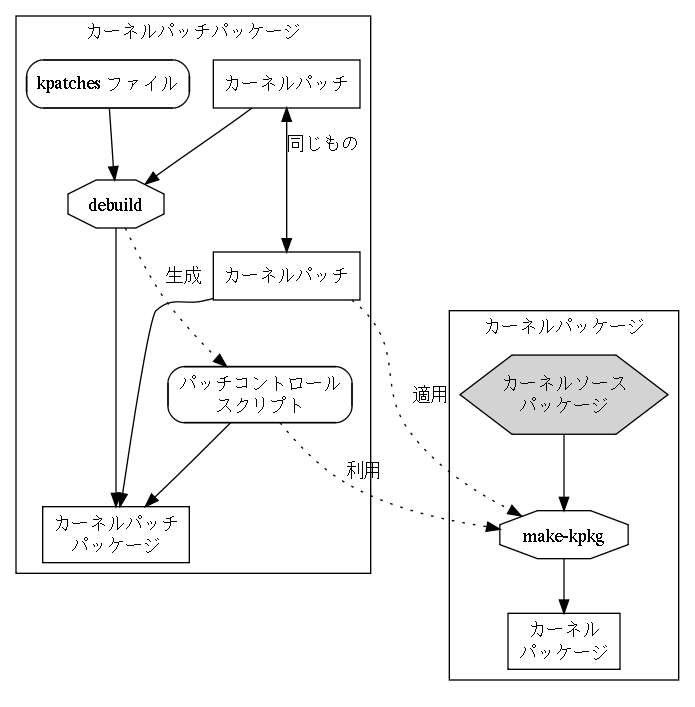
\includegraphics[width=0.8\hsize]{image200807/kpatch0.png}
 \end{center}
 \caption{Linux カーネルパッチ の Debian パッケージの仕組み}
 \label{fig:kpatch0}
\end{figure}

\subsection{パッケージ作成前の準備}

\subsubsection{dh-kpatches パッケージのインストール}
\index{debhelper}
\index{dh-kpatches}
dh-kpatches を使って、作成されたパッケージを使うことにより、make-kpkg コマンド \footnote{Debian でカーネルパッケージを作成
するためのコマンド。kernel-package パッケージで提供されている。} 
でカーネルパッチパッケージで提供しているパッチを適用した Linux カーネルパッケージが作成できるようになります。
パッケージ作成サポート用として、dh-make をインストールしておくと良いでしょう。dh-make を使うことによって、パッケージの
雛形を容易に作成することができます。
\begin{commandline}
$ sudo apt-get update
$ sudo apt-get install dh-kpatches dh-make build-essential
\end{commandline}



\subsubsection{パッチの用意}
まず、カーネル向けのパッチを作成する必要があります。開発者によっては、既にパッチがカーネルバージョン毎に用意されている事もありますが、
最近では、Linus のツリーに容易に追従できるように、Gitを使ってソースコードが管理されている場合が多いです。
POHMELFS でも ソースコードは Git で管理されており、安定版のカーネル(この原稿を書いている時点では、Linux 2.6.25)に常に追従されています。
この差分を取得するには、Git リポジトリを取得し、git diff コマンド等で取り出せばよいでしょう。

\begin{commandline}
$ git clone http://tservice.net.ru/~s0mbre/archive/pohmelfs/pohmelfs.git
Initialized empty Git repository in /tmp/pohmelfs/.git/
got 37e1b82c0535386cf09b3821dff5e8cb5f9e26b4
walk 37e1b82c0535386cf09b3821dff5e8cb5f9e26b4
<snip>
$ cd pohmelfs
$ git tag
<snip>
v2.6.24-rc8
v2.6.25
v2.6.25-rc1
v2.6.25-rc2
<snip>
$ git diff v2.6.25 > ~/pohmelfs.diff
\end{commandline}
%$ --emacs font-lock

\subsubsection{ディレクトリの作成}

パッチが作成できたら、パッケージ作成用のディレクトリを作成し、その中にパッチファイルをコピーします。
ディレクトリ名は Debianのポリシーに合わせたもの(ソフトウェアまたは機能名-バージョン)にしておき、パッチファイル名は
パッチ機能名-カーネルバージョン にしておきます。これは、このようなファイル名を dh-kpatches が要求するためです。

\begin{commandline}
$ mkdir linux-patch-pohmelfs-20080707
$ cd linux-patch-pohmelfs-20080707
$ cp ../pohmelfs.diff pohmelfs-2.6.x
\end{commandline}

\subsection{dh\_make を使った雛形の作成}
パッケージ作成の準備ができたら、 dh\_make コマンドを使って雛形を作成します。
dh\_make にはカーネルパッチ用のサポートはないので、singleバイナリの雛形を作成する
オプションを指定して、作成します。-r オプションは \texttt{orig.tar.gz} ファイルを作成し、-s オプションは
シングルバイナリ用の雛形を出力します。
\begin{commandline}
$ dh_make -r -s
Maintainer name : Nobuhiro Iwamatsu
Email-Address   : iwamatsu@nigauri.org 
Date            : Mon, 07 Jul 2008 01:00:33 +0900
Package Name    : linux-patch-pohmelfs
Version         : 20080707
License         : blank
Using dpatch    : no
Type of Package : Single
Hit <enter> to confirm: 
Currently there is no top level Makefile. This may require additional tuning.
Done. Please edit the files in the debian/ subdirectory now. You should also
check that the linux-patch-pohmelfs Makefiles install into $DESTDIR and not in / . 
\end{commandline}

\subsection{debianディレクトリ内の変更}
dh\_make コマンドで カーネルパッチを Debian パッケージにするための雛形が作成できました。
これを元に内容を変更していきます。

\subsubsection{サンプルスクリプト等の削除}
dh\_make で作成されるサンプルスクリプトは必要ないので全て削除します。
また、 dirs ファイルや doc ファイルも必要ないため削除します。
\begin{commandline}
$ rm -rf ./debian/*.ex ./debian/*.EX ./debian/docs ./debian/dirs
\end{commandline}

\subsubsection{debian/copyright の修正}
パッチの情報に合わせて、debian/copyright の修正を行います。
pohmelfs の場合は以下のように修正します。

\begin{commandline}
This package was debianized by Nobuhiro Iwamatsu <iwamatsu@nigauri.org> on
Mon, 07 Jul 2008 01:00:33 +0900.

It was downloaded from
        http://tservice.net.ru/~s0mbre/archive/pohmelfs/pohmelfs.git
This is Git repository. I made the difference of the latest committing a
patch from v2.6.25 tag.

Upstream Author(s):

    Evgeniy Polyakov <johnpol@2ka.mipt.ru>

Copyright:

    Copyright (C) 2008 Evgeniy Polyakov <johnpol@2ka.mipt.ru>

License:

 GPLv2

The Debian packaging is (C) 2008, Nobuhiro Iwamatsu <iwamatsu@nigauri.org> and
is licensed under the GPL, see `/usr/share/common-licenses/GPL'.

# Please also look if there are files or directories which have a
# different copyright/license attached and list them here.

\end{commandline}

\subsubsection{debian/README.Debian の修正}
debian/README.Debian ファイルに Debian で使うための HowToなどを書いておきましょう。
サポートしているカーネルバージョンや、カーネルイメージの作成方法などを書いておくのが一般的
なようです。

\begin{commandline}
linux-patch-pohmelfs for Debian
-------------------------------

This patch is pohmelfs support patch for Debian Linux kernel. 
You can try with linux-source-2.6.25 package. 

- How to use
  $ sudo apt-get install linux-source-2.6.25 libncurses-dev kernel-package
  $ cd /usr/src ; tar -xjf linux-source-2.6.25.tar.bz2 ; cd linux-source-2.6.25
  $ make-kpkg clean
  $ cp /boot/config-2.6.25-2-686 .config
  $ make menuconfig
  $ make-kpkg --rootcmd fakeroot --append-to-version -pohmelfs --revision 0.1 --added_patches=pohmelfs kernel-image

 -- Nobuhiro Iwamatsu <iwamatsu@nigauri.org>  Mon, 07 Jul 2008 01:00:33 +0900

\end{commandline}

\subsubsection{debian/control の修正}
次に debian/control ファイルを修正します。
注目すべきところは、作成されるパッケージで指定してある、{\bf Depends: \$\{kpatch:Depends\}}です。
ここで kpatch:Depends を指定することによって、カーネルパッチパッケージを使った
カーネル作成に必要な依存パッケージを置き換えてくれます。
また、ソースパッケージの {\bf Build-Depends} に {\bf dh-kpatches パッケージ} を追加する事を忘れないようにしましょう。

\begin{commandline}
Source: linux-patch-pohmelfs
Section: devel
Priority: extra
Maintainer: Nobuhiro Iwamatsu <iwamatsu@nigauri.org>
Build-Depends: debhelper (>= 6), dh-kpatches
Standards-Version: 3.8.0.1
Homepage: http://tservice.net.ru/~s0mbre/old/?section=projects&item=pohmelfs

Package: linux-patch-pohmelfs
Architecture: all
Depends: ${kpatch:Depends}
Description: POHMELFS kernel patch
 POHMELFS stands for Parallel Optimized Host Message Exchange Layered File System.
 Development status can be tracked in filesystem section.
 This is a high performance network filesystem with local coherent cache of data
 and metadata.
 Its main goal is distributed parallel processing of data. Network filesystem is a
 client transport.
 POHMELFS protocol was proven to be superior to NFS in lots (if not all, then it
 is in a roadmap) operations.
\end{commandline}

\subsubsection{debian/changelog の修正}
dch コマンドを使って debian/changelog ファイルを修正します。
\begin{commandline}
$ dch
linux-patch-pohmelfs (20080707-1) unstable; urgency=low

  * Initial release                                          

 -- Nobuhiro Iwamatsu <iwamatsu@nigauri.org>  Mon, 07 Jul 2008 01:25:37 +090
\end{commandline}

\subsubsection{kpatches ファイル}

どのパッケージ内に収録されているパッチをどのカーネルバージョンに当てればいいのかなどを
コントロールするためのファイル kpatches を用意する必要があります。
このファイルは以下のようなフォーマットになっており、
カーネルバージョン毎に Patch-file と Kernel-version の項目を追加する必要があります。
また、このファイルを {\bf パッケージ名.kpatches} として 名前を変更する必要があります。

\begin{commandline}
Patch-name: POHMELFS patch
Patch-id: pohmelfs <-- make-kpkg の --added-patches で指定するパッチ名 
Architecture: all <-- サポートするアーキテクチャ
Path-strip-level: 1

Patch-file: pohmelfs-2.6.x <-- パッチファイル名
Kernel-version: 2.6.25 <-- パッチがサポートするカーネルバージョン
\end{commandline}

\subsubsection{\texttt{debian/rules} ファイルの修正}
\texttt{debian/rules} ファイルで注意する点として、 install ターゲットで、
dh\_installkpatches を指定する必要があります。dh\_installkpatches で
カーネルパッチが kpatches ファイルと共ににパッケージ作成用の一時ディレクトリにコピーされます。

\begin{commandline}
#!/usr/bin/make -f

build: build-stamp
build-stamp:
        dh_testdir
        touch build-stamp

clean:
        dh_testdir
        dh_testroot
        rm -f build-stamp
        dh_clean

install: build
        dh_testdir
        dh_testroot
        dh_clean -k
        dh_installdirs
        dh_installkpatches

# Build architecture-independent files here.
binary-indep: build install
        dh_testdir
        dh_testroot
        dh_installchangelogs
        dh_link
        dh_strip
        dh_compress
        dh_fixperms
        dh_installdeb
        dh_shlibdeps
        dh_gencontrol
        dh_md5sums
        dh_builddeb

# Build architecture-dependent files here.
binary-arch: binary-indep

# We have nothing to do by default.

binary: binary-indep binary-arch
\end{commandline}

\subsubsection{ディレクトリ構成}
最終的な debian ディレクトリの構成をチェックしてみます。
以下のようになっているとよいでしょう。
\begin{commandline}
linux-patch-pohmelfs-20080707/
|-- debian
|   |-- README.Debian
|   |-- changelog
|   |-- compat
|   |-- control
|   |-- copyright
|   |-- linux-patch-pohmelfs.kpatches
|   `-- rules
`-- pohmelfs-2.6.x
\end{commandline}

\subsection{パッケージのビルドおよびインストール}
パッケージのビルドを行う際には、通常のパッケージ作成と変わりません。
debuild などを使ってパッケージの作成を行ってください。
作成されたパッケージをインストールすると、\url{/usr/src/kernel-patches} にパッチと制御用のスクリプトが
インストールされます。make-kpkg コマンドはこのディレクトリを参照し、パッチを適用します。
\begin{commandline}
% debuild
% sudo dpkg -i ../linux-patch-pohmelfs_20080707-1_all.deb
\end{commandline}

\subsection{パッケージのテスト}
カーネルパッチパッケージのテストは、カーネルソースコードに
パッチを当て、カーネルがコンパイルできるか、確認する必要があります。
また、Debian の場合は、Debian と kernel.org で配布しているカーネルの2種類を考慮する必要がありますが、
前者の方をテストしていれば十分でしょう。
インストールしたカーネルパッチパッケージを使って、カーネルをコンパイルするには、
make-kpkg コマンドの--added\_patches のオプションを使って、パッチを指定します。
パッチが当たっているかソースを確認し、カーネルのコンパイルが正常に行われているか確認しましょう。
また、作成された カーネルパッケージを実際にインストールし、テストを行うことも重要です。

\begin{commandline}
$ sudo apt-get install linux-source-2.6.25 libncurses-dev kernel-package
$ cd /usr/src ; tar -xjf linux-source-2.6.25.tar.bz2 ; cd linux-source-2.6.25
$ make-kpkg clean
$ cp /boot/config-2.6.25-2-686 .config
$ make menuconfig
$ make-kpkg --rootcmd fakeroot --append-to-version -pohmelfs --revision 0.1 --added_patches=pohmelfs kernel-image
\end{commandline}

\subsection{パッケージのアップデート方法}
いまのところ、カーネルパッチソースパッケージのアップデート方法が決まっていません。
適当なディレクトリを作成して、uupdate コマンドを実行するのが一番容易と思われます。
将来的には、パッチを指定することによって、ソースパッケージをアップデートできるように
したいと考えています。

\subsection{まとめ}
以上の手順を使うと、Linux カーネルパッチの Debian パッケージを作成することができます。
しかし、このままではかなり手間がかかりますので、今回の成果物をまとめ、
dh-make で Linux カーネルパッチパッケージの雛形が作成できるように機能を追加しました(\#304688)。
\footnote{dh-make 0.47でパッチが取り込まれ、利用可能になりました。}\index{dh-make}
このパッチが取り込まれると、dh-make を使うことにより、より簡単に Linux カーネルパッチパッケージ
が作成できるようになるでしょう。また、cdbsを使った方法をまだ調べていないので、調べようと思っています。
ちなみに、pohmelfs は linux-2.6.27 or 2.6.28 に取り込まれるようです。よかったよかった。
\index{pohmelfs}

\dancersection{Linux カーネルモジュールの Debian パッケージ作成}{岩松 信洋}
\label{sec:kmod}
\index{kmod}
\index{Linux Kernel Module}

\subsection{はじめに}
今回は video データloopback 用 Linux カーネルモジュール、vloopback を題材にして、
Linux カーネルモジュールの Debian パッケージ作成方法を説明します。

\subsection{なぜカーネルモジュールソースコードをパッケージ化するのか}
Linux の カーネルモジュールソースコードをパッケージ化する理由の一つとして、
カーネルバージョンに合わせたドライバを管理する手間が省ける事と
モジュールドライバコンパイルフロントエンド module-assistant 
による 操作のしやすさが大きいでしょう。このソフトウェアを使うことによって、
容易にモジュールのコンパイルおよびインストールを行う事ができます。
現時点では、カーネルバージョンが上がる度にコンパイルする必要がありますが、
パッケージ化しておくと、ある程度まで自動化できるため、アップデートも容易になります。

\subsection{カーネルモジュールパッケージの仕組み}
パッケージの作り方の説明の前にカーネルモジュールパッケージの仕組みについて説明します(図\ref{fig:mod0})。
カーネルモジュールパッケージは 内部に カーネルモジュールソースコードとコンパイルするための Makefile(\texttt{debian/rules})
と、control ファイル(debian/control に相当するもの)を固めたものである ドライバソースイメージを持っています 。
このドライバソースイメージは、実際は Debian ソースパッケージと構成は同じになっており、 bzip2 で圧縮したものになります。 
カーネルモジュールパッケージをインストールすると、\texttt{/usr/src/} に ドライバソースイメージが置かれ、\texttt{module-assistant} が
このファイルを\texttt{/usr/src/modules} ディレクトリ以下、ビルド毎に展開し、ドライバ用の Debian パッケージビルドを行います。
作成された パッケージは \texttt{/usr/src} に置かれます。
モジュールソースパッケージは、このドライバソースイメージを作成し、\texttt{module-assistant} と連携できる機能を
提供します。

\begin{figure}[h]
 \begin{center}
  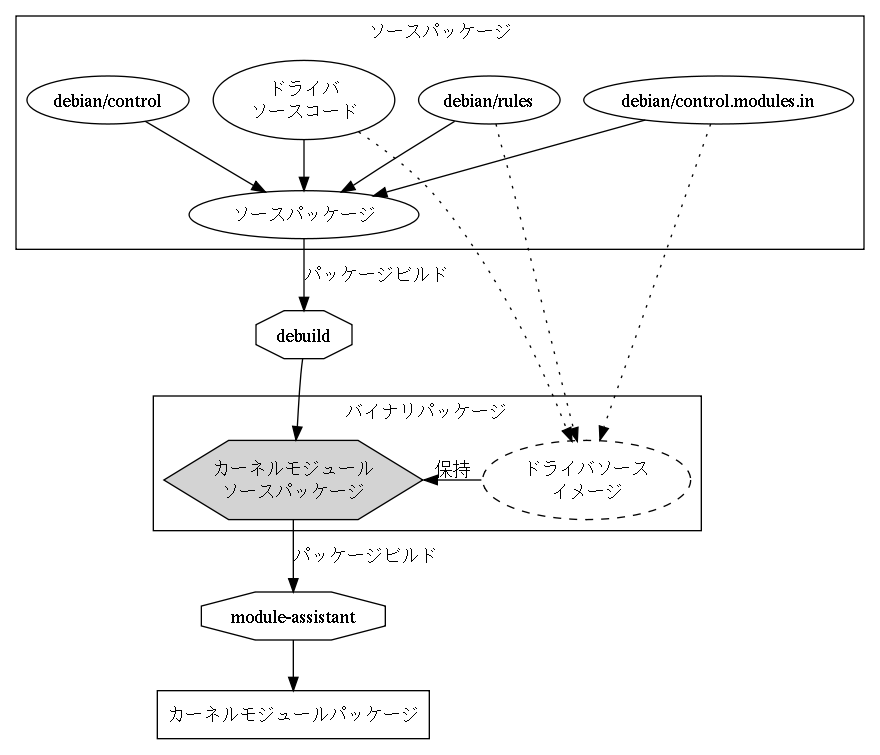
\includegraphics[width=0.8\hsize]{image200807/kmod0.png}
 \end{center}
 \caption{カーネルモジュールパッケージの仕組み}
 \label{fig:mod0}
\end{figure}

\subsection{ドライバソースコードの取得と展開}
\texttt{vloopback} は \texttt{flashcam} という フリーソフトウェアと共に提供されています。
今回は、\texttt{vloopback} のソースコードだけをターゲットにするので、ソースコードを
取り出します。
\begin{commandline}
$ wget http://www.swift-tools.net/Flashcam/flashcam-1.1.tgz
$ tar -xzf flashcam-1.1.tgz
$ cp -rf flashcam-1.1/vloopback-1.1.2 .
$ cd vloopback-1.1.2
\end{commandline}

\subsection{dh\_make を使った雛形の作成}
パッケージ作成の準備ができたら、 \texttt{dh\_make} コマンドを使って雛形を作成します。
\texttt{dh\_make} には、カーネルモジュールの雛形を作成するオプション \texttt{-k / --kmod} が提供されています。

\begin{commandline}
$ dh_make -k -r 
Maintainer name : Nobuhiro Iwamatsu
Email-Address   : iwamatsu@nigauri.org 
Date            : Tue, 15 Jul 2008 23:21:23 +0900
Package Name    : vloopback
Version         : 1.1.2
License         : blank
Using dpatch    : no
Type of Package : Kernel Module
Hit <enter> to confirm: 
Done. Please edit the files in the debian/ subdirectory now. You should also
check that the vloopback Makefiles install into $DESTDIR and not in / .
\end{commandline}

\subsection{debianディレクトリ内の変更}
Debian パッケージにするための雛形が作成できたので、これを元に内容を変更していきます。

\subsubsection{サンプルスクリプト等の削除}
dh\_make で作成されるサンプルスクリプトは必要ないので全て削除します。
\begin{commandline}
$ rm -rf ./debian/*.ex ./debian/*.EX
\end{commandline}

\subsubsection{debian/copyright の修正}
パッチの情報に合わせて、debian/copyright の修正を行います。
vloopback の場合は以下のように修正します。

\begin{commandline}
This package was debianized by Nobuhiro Iwamatsu <iwamatsu@nigauri.org> on
Tue, 15 Jul 2008 23:21:23 +0900.

It was downloaded from <http://www.swift-tools.net/Flashcam/flashcam-1.1.tgz>

Upstream Author(s):

    Olivier Debon <olivier@debon.net>

Copyright:

    Copyright (C) 2008 Olivier Debon <olivier@debon.net>

License:

    GPLv2

The Debian packaging is (C) 2008, Nobuhiro Iwamatsu <iwamatsu@nigauri.org> and
is licensed under the GPL, see `/usr/share/common-licenses/GPL'.

# Please also look if there are files or directories which have a
# different copyright/license attached and list them here.
\end{commandline}

\subsubsection{debian/README.Debian の修正}
debian/README.Debian ファイルを修正します。
雛形がある程度書いておいてくれているので、あまり修正する必要はありません。
確認した Linux カーネルバージョンなどを書いておくと良いかもしれません。

\begin{commandline}
vloopback for Debian
--------------------

Please see ./README for a description of the vloopback software.

The Debian vloopback source package provides two packages,

 vloopback-source, which provides the source for the kernel modules

The vloopback-source package can be used in several ways,

 - Using the make-kpkg(1) command provided by the kernel-package Debian
   package. This will produce a corresponding vloopback-modules package for
   the Debian kernel-image package that you are using. This is "the Debian
   way". See the "modules_image" section of the make-kpkg(1) man page.

 - Changing to the /usr/src/modules/vloopback/ directory and building as
   the README file instructs using "make; make install". This will build
   and install a module specific to the system you are building on and is
   not under control of the packaging system.

 -- Nobuhiro Iwamatsu <iwamatsu@nigauri.org>  Tue, 15 Jul 2008 23:21:23 +0900
\end{commandline}

\index{vloopback}

\subsubsection{debian/control の修正}
次に debian/control ファイルを修正します。
dh\_make で作成した場合は、vloopback-utils といった、ドライバをサポートするための
パッケージを作成するエントリがあります。
ソースコードにツールが含まれている場合は、このエントリを使って、ツール用のパッケージを
作成できるようになっています。今回は必要ないので削除します。

以下に debian/control ファイルの例を示します。
\begin{commandline}
Source: vloopback
Section: graphics
Priority: extra
Maintainer: Nobuhiro Iwamatsu <iwamatsu@nigauri.org>
Build-Depends: debhelper (>= 7), bzip2
Standards-Version: 3.8.0.1
Homepage: http://www.swift-tools.net/Flashcam/

Package: vloopback-source
Architecture: all
Depends: module-assistant, debhelper (>= 7), make, bzip2
Description: Source for the vloopback driver.
 This package provides the source code for the vloopback kernel modules.
 The vloopback package is also required in order to make use of these
 modules. Kernel source or headers are required to compile these modules.
\end{commandline}

\subsubsection{debian/changelog の修正}
dch コマンドを使って debian/changelog ファイルを修正します。
\begin{commandline}
$ dch
vloopback (1.1.2-1) unstable; urgency=low

  * Initial release

 -- Nobuhiro Iwamatsu <iwamatsu@nigauri.org>  Tue, 15 Jul 2008 23:21:23 +0900
\end{commandline}

\subsubsection{control.modules.in ファイルの修正}
カーネルモジュールパッケージのソースパッケージは 2つの control ファイルを持ちます。
一つは、元のソースパッケージと、作成されるカーネルモジュールソースパッケージの情報が書かれた control ファイル、
もう一つは、カーネルモジュールパッケージの情報が書かれた control.modules.in ファイルです。
ソースパッケージ$\rightarrow$カーネルモジュールソースパッケージ$\rightarrow$カーネルモジュールパッケージの
順で作成されるので、ユーザは リポジトリからカーネルモジュールソースパッケージを取得し、module-assistant を使って
実際のカーネルモジュールパッケージを作成します。そして、ユーザは カーネルモジュールパッケージをインストールして
利用します。

このファイルの中ではカーネルのバージョンによって置換される文字列が \texttt{\_KVERS\_} という文字列になっています。
{\bf control.modules.in} は {\bf module-assistant} などにより処理され、
各Linux カーネルバージョン用の内容に変更されます。

以下に  debian/control.modules.in ファイルの例を示します。
\begin{commandline}
Source: vloopback
Section: graphics
Priority: optional
Maintainer: Nobuhiro Iwamatsu <iwamatsu@nigauri.org>
Build-Depends: debhelper (>= 7), bzip2
Standards-Version: 3.8.0.1

Package: vloopback-modules-_KVERS_
Architecture: any
Provides: vloopback-modules
Description: vloopback modules for Linux (kernel _KVERS_).
 This package contains the set of loadable kernel modules for the
 <description>.
 .
 This package contains the compiled kernel modules for _KVERS_
 .
 If you have compiled your own kernel, you will most likely need to build
 your own vloopback-modules. The vloopback-source package has been
 provided for use with the Debian's module-assistant or kernel-package
 utilities to produce a version of vloopback-modules for your kernel.
\end{commandline}

\subsubsection{debian/rules ファイルの修正}

dh\_make で作成された、\texttt{debian/rules} ファイルは パッケージ作成用のターゲット(build/install/clean)と、
ドライバパッケージ作成用のターゲット binary-modules/kdist\_clean が用意されています。
これらのターゲットの中を修正します。
\begin{commandline}
#!/usr/bin/make -f

psource:=vloopback-source
sname:=vloopback

# prefix of the target package name
PACKAGE=vloopback-modules
# modifieable for experiments or debugging m-a
MA_DIR ?= /usr/share/modass
# load generic variable handling
-include $(MA_DIR)/include/generic.make
# load default rules, including kdist, kdist_image, ...
-include $(MA_DIR)/include/common-rules.make

kdist_config: prep-deb-files
kdist_clean: clean
	$(MAKE) $(MFLAGS) -f debian/rules clean

configure: configure-stamp
configure-stamp:
	dh_testdir
	# Add here commands to configure the package.

	touch configure-stamp

build-arch: configure-stamp  build-arch-stamp
build-arch-stamp: 
	dh_testdir

	# Add here command to compile/build the package.
	# $(MAKE)

	touch $@

#k = $(shell echo $(KVERS) | grep -q ^2.6 && echo k)

# during a normal build
binary-modules:
	dh_testroot
	dh_clean -k
	dh_installdirs lib/modules/$(KVERS)/misc

	# Build the module
	$(MAKE) KVER=$(KVERS) KSRC=$(KSRC)

	# Install the module
	cp vlooopbackko debian/$(PKGNAME)/lib/modules/$(KVERS)/misc

	dh_installdocs
	dh_installchangelogs
	dh_compress
	dh_fixperms
	dh_installdeb
	dh_gencontrol -- -v$(VERSION)
	dh_md5sums
	dh_builddeb --destdir=$(DEB_DESTDIR)
	dh_clean -k
\end{commandline}

\begin{commandline}
build-indep:  configure-stamp build-indep-stamp
build-indep-stamp: 
	dh_testdir
	touch $@

build: build-arch build-indep

clean: 
	dh_testdir
	rm -f build-arch-stamp build-indep-stamp configure-stamp
	dh_clean

install: DH_OPTIONS=
install: build
	dh_testdir
	dh_testroot
	dh_clean -k
	dh_installdirs

	# Create the directories to install the source into
	dh_installdirs -p$(psource)  usr/src/modules/$(sname)/debian

	# Copy only the driver source to the proper location
	cp vloopback.c  debian/$(psource)/usr/src/modules/$(sname)/.
	# Copy the needed debian/ pieces to the proper location
	cp debian/*modules.in* \
		debian/$(psource)/usr/src/modules/$(sname)/debian
	cp debian/rules debian/changelog debian/copyright \
		debian/compat debian/$(psource)/usr/src/modules/$(sname)/debian/
	cd debian/$(psource)/usr/src && tar c modules | bzip2 -9 > $(sname).tar.bz2 && rm -rf modules

	# Add here commands to install the package into debian/vloopback.
	# $(MAKE) DESTDIR=$(CURDIR)/debian/vloopback install

	dh_install

# Build architecture-independent files here.
# Pass -i to all debhelper commands in this target to reduce clutter.
binary-indep: build install
	dh_testdir -i
	dh_testroot -i
	dh_installchangelogs  -i
	dh_installdocs -i
	dh_installexamples -i
	dh_installman -i
	dh_link -i
	dh_compress -i
	dh_fixperms -i
	dh_installdeb -i
	dh_gencontrol -i
	dh_md5sums -i
	dh_builddeb -i

# Build architecture-dependent files here.
binary-arch: build install
	dh_testdir -s
	dh_testroot -s
	dh_installdocs -s
	dh_installinfo -s
	dh_installchangelogs  -s
	dh_compress -s
	dh_fixperms -s
	dh_installdeb -s
	dh_shlibdeps -s
	dh_gencontrol -s
	dh_md5sums -s
	dh_builddeb -s

binary: binary-indep binary-arch
.PHONY: build clean binary-indep binary-arch binary install configure binary-modules \
        kdist kdist_configure kdist_image kdist_clean

\end{commandline}

\subsection{パッケージのビルドおよびインストール}
パッケージのビルドを行う際には、通常のパッケージ作成と変わりません。
debuild などを使ってパッケージの作成を行ってください。
作成されたパッケージをインストールすると、\texttt{/usr/src/modules} にドライバソースイメージが
インストールされます。
\begin{commandline}
% debuild
% sudo dpkg -i ../vloopback-source_1.1.2-1_all.deb
\end{commandline}

\subsection{モジュールパッケージの作成}
\subsubsection{module-assistantを使ったコンパイル}
ドライバパッケージのコンパイルには module-assistant \index{module-assistant}
コマンドを利用します。
このコマンドは GUIを持っており、GUIでドライバのコンパイルやコンパイル環境の
アップデートを行う事ができます。
GUIで選択できるドライバ群は \texttt{module-assistat}パッケージ内で持っているリスト(\ref{/usr/share/modass/compliant.list})のみ
が対象になっているため、新しく作成したものは選択できません。
このような場合は、モジュール名を指定することによってコンパイル可能です。
コンパイルした後には、\ref{/usr/src/} ディレクトリ以下にカーネルモジュールパッケージが作成されるので、
このパッケージをインストールすることによって、ドライバがコンパイルした Linux カーネルのバージョン上で
利用できるようになります。また、module-assistant は作成したパッケージの自動インストール機能\footnote{a-i オプション}
もあります。

\begin{commandline}
$ sudo m-a build vloopback
Extracting the package tarball, /usr/src/vloopback.tar.bz2, please wait...
/usr/bin/make clean
make[1]: ディレクトリ `/usr/src/modules/vloopback' に入ります

<snip>

make[3]: ディレクトリ `/usr/src/linux-headers-2.6.25-2-686' に入ります
  CC [M]  /usr/src/modules/vloopback/vloopback.o
  Building modules, stage 2.
  MODPOST 1 modules
  CC      /usr/src/modules/vloopback/vloopback.mod.o
  LD [M]  /usr/src/modules/vloopback/vloopback.ko
make[3]: ディレクトリ `/usr/src/linux-headers-2.6.25-2-686' から出ます
make[2]: ディレクトリ `/usr/src/modules/vloopback' から出ます
# Install the module
cp vloopback.ko debian/vloopback-modules-2.6.25-2-686/lib/modules/2.6.25-2-686/misc
dh_installdocs
dh_installchangelogs
dh_compress
dh_fixperms
dh_installdeb
dh_gencontrol -- -v1.1.2-1+2.6.25-6
dh_md5sums
dh_builddeb --destdir=/usr/src
dpkg-deb: `/usr/src/vloopback-modules-2.6.25-2-686_1.1.2-1+2.6.25-6_i386.deb' にパッケージ \
 `vloopback-modules-2.6.25-2-686' を構築しています。
dh_clean -k

<snip>
\end{commandline}

\subsubsection{make-kpkgを使ったコンパイル}  
module-assistant 以外にも make-kpkg の --added-modules オプションを使うことによって
コンパイルすることができます。しかし、make-kpkg の場合にはドライバソースイメージを展開してくれない
ので、手動で展開する必要があります。
kernel-package はカーネルパッケージ専用と考えたほうがよさそうです。
(そのために module-assistant ができたので。)
\index{make-kpkg}

\subsection{まとめ}
今回は dh\_make からの作成でしたが、cdbs を使うともっと簡単かつ簡潔に作成することができます。
過去の勉強会資料にちょっとだけ載っているので、参考にしてください。
しかし、カーネルドライバ側の \texttt{debian/rules} は cdbs での対応が行われていないので、対応する
必要があるでしょう。
あと、最近はドライバも linus ツリーに取り込まれやすくなったのですが、
Linuxのリリース間隔などを考えると、新しいドライバは簡単に使えるものではありません。
新しいドライバを早く使いたい人には、ドライバパッケージ群が重要なパッケージになってくると思います。
そのためには、今後はこれらのパッケージをどのようにメンテナンスしていくかなどについて考えていく
必要がありそうです。

\subsection{おまけ}
module-assistant でサポートされているパッケージがどれぐらいコンパイルできるのか調べてみました。
アーキテクチャは i386 、ディストリビューションは sid です。パッケージは \ref{/usr/share/modass/compliant.list} にかかれているものです。
結果は82個中、コンパイルOK: 22/ コンパイルNG: 22/ パッケージなし: 38 になりました。パッケージなしなのは、module-assistant のリストがメンテナンスされていなからだと思います。あとは、アーキテクチャ非対応など。
既にカーネルにマージされているものがけっこうあり、コンパイルエラーは各メンテナがサボっているのでしょう。
これらは今後BTSしていくつもりです。


\dancersection{みんなも Debian GNU/Hurd を使おうよ!}{山本 浩之}
\label{sec:gnuhurdminnnade}
\index{Hurd} 

いきなり実機で Hurd を使いたい、と言う人は稀でしょうし、Hurd のインストーラ自身も問題を抱えているらしく、私も実機への直接のインストールは成功していません。しかし仮想環境でなら、気軽で、簡単に使えます。
今日は Debian GNU/Hurd の VMware 上での利用を紹介してみます。

まず、インストールの様子を見てみましょう。インストーラは、かなり昔の debian-installer を彷彿とさせ、懐かしむ人もいるでしょう。
実際、woody の d-i をベースとしており、最近の d-i (lenny beta2 など)へは付いて行けてはいません。

Hurd のインストーラ CD は Linux カーネルで動いており、その中の /target として Hurd 環境を展開していきます。
残念ながら woody は kernel 2.2.20 だったため、128 GB 以上のディスク (Big Drive) への対応はされていません。
また、私が試した限りですが、30 GB より大きなパーティションには正常にインストールできないようです。実際、40 GB と 60 GB 
のディスクイメージにインストールした場合、インストールは終わったように見えますが、40 GB の時は Hurd がシングルユーザでもブートせず、
60 GB の時はなぜかシングルユーザによる最初のブートはできましたが、ファイルのパーミッションが  \verb!? ---------! となっていてアクセスできない状態でした。

では実際に 30 GB のディスクイメージにインストールしてみましょう。
まずインストール CD イメージからブートし、キーボードの選択をしたら、パーティションを決めます。この時点ではカーネルは Linux のままですので、
hda1 とか hda5 とかの見慣れたパーティション指定ができます。この時、swap を必ず作成して下さい。swap を作ることを公式にも推奨されていますが、
私が swap を作らずにインストールしたところ、まったくブートしませんでした。ここでは swap を取った残りを全て / としておきます。
Hurd の対応フォーマットは、残念ながらいまだに ext2 のみです。パーティションを決めたら、フォーマットします。swap は Linux と全く同じですが、
/ は mke2fs を実行する際に -o hurd を引数として与えることだけ異なっています。
フォーマットしたら base.tgz の展開です。このあたりは昔の d-i を経験したかたならお手のものでしょう。

ただ、Hurd の d-i としての問題点は、grub を直接インストールできないことにあります。Hurd に対応したブートローダは、今のところ、grub だけなのですが、
インストール CD には grub を入れるメニューがありません。これは既に Linux を入れていて grub をインストール済みなかたが多いためなのか、
woody の d-i の問題点なのかは知りません。そこで、grub の FD あたりを用意しておき、別途 grub をインストールしなくてはなりません。
最近は FDD を持たないマシンが増えており、このあたりは改善すべき点だと思います。

grub をインストールし、menu.lst には
\begin{commandline}
default=0
timeout=10

title  Debian GNU/Hurd
root (hd0,0)
kernel (hd0,0)/boot/gnumach.gz root=device:hd0s1
module (hd0,0)/hurd/ext2fs.static --multiboot-command-line=${kernel-command-line} \
--host-priv-port=${host-port} --device-master-port=${device-port} \
--exec-server-task=${exec-task} -T typed ${root} $(task-create) $(task-resume)
module (hd0,0)/lib/ld.so.1 /hurd/exec $(exec-task=task-create)
boot

title  Debian GNU/Hurd (single user)
root (hd0,0)
kernel (hd0,0)/boot/gnumach.gz root=device:hd0s1 -s
module (hd0,0)/hurd/ext2fs.static --multiboot-command-line=${kernel-command-line} \
--host-priv-port=${host-port} --device-master-port=${device-port} \
--exec-server-task=${exec-task} -T typed ${root} $(task-create) $(task-resume)
module (hd0,0)/lib/ld.so.1 /hurd/exec $(exec-task=task-create)
boot
\end{commandline}
と書きます。 (hd0,0)/boot/gnumach.gz がカーネルで、hd0s1 とは Linux の hda1 (プライマリマスタ、第一パーティション) のことです。
Hurd の / には /hurd と言うディレクトリが存在しており、この中に Hurd 特有のモジュールなどが存在しています。
ここでは (hd0,0)/hurd/ext2fs.static と言う ext2 フォーマットを読み込むモジュールが指定されています。

ここまで行けば、インストーラを再起動し、まずシングルユーザで Hurd をブートし、
\begin{commandline}
# ./native-install
\end{commandline}
で /native-install スクリプトを実行、再度シングルユーザで再起動、再度 /native-install スクリプトを実行で終わりです。

ここまでの工程が面倒なかたには、\texttt{debian-hurd-k16-qemu.img.tar.gz} と言う \texttt{qemu} 用の素晴らしいイメージが配布されていますので、
これが利用できます。特に FDD が無くて grub のインストールが面倒なかたにお薦めです。
\begin{commandline}
$ wget http://ftp.debian-ports.org/debian-cd/K16/debian-hurd-k16-qemu.img.tar.gz
$ tar zxvf debian-hurd-k16-qemu.img.tar.gz
$ qemu-img convert debian-hurd-k16-qemu.img -O vmdk
\end{commandline}
さて、インストールも終わったところで、実際にブートしてみましょう。普通にブートすれば
\begin{commandline}
login >
\end{commandline}
とプロンプトが出てきますので、'login root' でログインします。最初はパスワードはかかっていません。

まずはとにかく、ネットワークに繋ぐために設定します。Hurd には /sbin/ifconfig などが無く、settrans コマンドで設定します。
\begin{commandline}
# settrans -fgap /servers/socket/2 /hurd/pfinet -i eth0 -a 192.168.1.3 -g 192.168.1.1 -m 255.255.255.0
\end{commandline}
あとは Linux と同様に、/etc/resolv.conf に
\begin{commandline}
nameserver 192.168.1.1
\end{commandline}
とか書いてやるだけでネットワークに繋がります。

Debian GNU/Hurd のユーザランドは Debian そのもので、ほとんどは Linux の知識で間に合います。ただし、まだディベロッパやメンテナなどに Hurd が浸透しておらず、FTBFS (Failure To Build From Source) が多数あり、多くのパッケージが使えない状態です。
特に多いエラーは、PATH\_{}MAX (MAXPATHLEN) の未定義エラーです。Hurd には Linux などと違い、パスの最大文字数を制限すると言う概念が無いらしく、文字どおり未定義となっております。ディベロッパやメンテナの人には、自分のパッケージが Hurd でビルドできるか、是非試していただきたいものです。

Let's enjoy Hurd!


% tokyoresume200808 / 43 

\dancersection{Debconf 8}{岩松 信洋}
\label{sec:debconf8}
\index{debconf8}

勉強会として、今回の Debconf 開催地である アルゼンチンからIRCを使って行われました。内容を以下に報告します。

\subsection{当日のアジェンダ}
\begin{enumerate}
\item 22:00-  Debconf 参加者 の 今回の意気込み
\item 22:30-  Debconf 参加者 への Debconf 質問コーナー
\end{enumerate}

\subsection{参加者}
\begin{itemize}
\item debconf側

 上川さん(dancer)

\item 日本側
kmuto, henrich, yamamoto, aya, honjo, risou, mkouhei, ake, iwamatsu
\end{itemize}

\subsection{参加者への質問}
Debconf 参加者への質問ということで、以下の質問があり、参加者から回答を得ることができました。
質問内容 (質問者名) という形式になっています。

\begin{enumerate}
\item 無事にたどりつけましたか (kmuto)

  予約待ちしていたバスが予約できていなかったので、retiro 経由でバス8時間、合計40時間の行程でした。今回しかも、san francisco からの旅程なので、日本からいってたら死ねる (dancerj) 

\item wife様がgeekどもを見て一言 (匿名)

  「ほどほどにね」 

\item 日本からは(そもそも)誰が行っているのですか?(AyaKomuro)

   上川さん夫妻です(奥様可哀想と言う声もあるような…「アルゼンチンに旅行にいく、としか説明していなかった・・・」) 

\item 今回のDebconfで期待しているセミナー/レクチャーは何ですか?(AyaKomuro)

   「基本的に期待していないので、Hacklab にずっといるつもりです。」 

\item Debconf@Argentinaならではのこれは!?を教えてください(AyaKomuro)

  \begin{itemize}
    \item keysigning party に出ないつもりなので個別にkeysigningをする。
    \item qemu maintainer groupに強制収容された、qemubuilder ハックした
    \item あと Don armstrongをつかまえてBTS SOAP のインタフェースのバグを直してもらうかな
  \end{itemize} 
\item 日本で debconf 開いたら来たいよーって人はどのくらいいるのでしょうか? (henrich)
   
  「明日、19:00 からdebconf10会議がある。」 

\item ごはんはおいしいのかな (kmuto)

   「ごはんうまいっす。かなり。いけてる。朝飯からケーキ。牛メインですね。港町なので魚もある。野菜はすくな目かな。パンはそうでもないです。debconf の会場のそとで食事したら多分肉肉してるんだろうけど、ホテルの食事はそうでもないです。」 
\item 日本の Debian 関係者に何か一言ないか。(henrich)

  無回答
\item Lenny で DDTP のエンコードによる文字化け問題は解決の見込みがあるのか (henrich)

  無回答
\item unzip の表示がおかしくなる問題について、Ubuntu のメンテナとの協業で解決してはもらえないのか。大変この問題を憂いている。(henrich)
       
    ack. 
\item Ubuntu のような LoCo (Local Community) などは検討していないのか? (henrich) 
   
  無回答
\end{enumerate}

\dancersection{Debian 温泉}{岩松 信洋}
\label{sec:debian-onsen}
\index{debian-onsen}

2008年8月16日はDebian 15 周年です。おめでとう! Debian 勉強会では、15周年を祝うために
有志で Debian 温泉と題した 合宿を行いました。以下に合宿レポートを紹介します。

\subsection{Debian 温泉の日程、場所、参加者}
今回は、Debian勉強会に参加された方から希望者を募って実験的に合宿を行う方式を取りました。
当初は伊豆の伊東温泉で行う予定でしたが、予定していた場所を予約できず、
急遽、草津温泉に変更なりました。伊東温泉を楽しみにしていた方、申し訳ございませんでした。

天気は雨。大雨に見舞われましたが、温泉にひきこもってハックするだけなので
天気はあまり関係ありません。しかし、一部の人が{\bf なぜか}雨で濡れたり、着替えをもってこなかったために
最悪な状態になってしまったようです。民宿の方がタオルを貸してくれたり、濡れてしまった靴から水を吸い出すために
新聞紙を提供してくれたおかげで、帰るころには乾いていたようです。民宿の方ありがとうございました。(見てないと思うけど。)

\begin{table}[h]
 \begin{center}
 {
   \begin{tabular}{l|l} \hline
     日程 & 2008年8月16日 - 8月17日  \\
     場所 & 草津/草津温泉 \\
     利用したところ & 民宿 美山 \footnote{\url{http://www.jalan.net/uw/uwp3000/uww3001.do?&rootCd=77&yadNo=351135}}\\
     宿泊費 & 8000円(夕食/朝食/入湯税込み)\\
     参加者 & henrich, yamamoto, mkouhei, nori1, tks, hibino, ake ,honjo, iwamatsu\\
   \end{tabular}
 }
 \caption{Debian 温泉の日程、場所、参加者}
 \label{onsen-data}
 \end{center}
\end{table}

\subsection{行われたこと、合宿成果}

今回の合宿の目的は以下のとおりです。

\begin{itemize}
\item Debian 15周年を祝う
\item 温泉に入る
\item Debian 開発
\item Debian 勉強会に関してのグループワーク/ワークショップを行う
\item Debian JP Project 理事 打ち合わせ
\end{itemize}

また、開発結果として、以下のものが行うことができました。

\begin{table}[h]
 \begin{center}
 {
   \begin{tabular}{l|l} \hline
     名前 & 開発結果  \\ \hline \hline
     henrich & po-debconf 翻訳 \\
     yamamoto & FDClone パッケージメンテナンス \\
     mkouhei & MacBook Air まわりのハック \\
     nori1 & Debian パッケージメンテナンス \\
     tks & V4L まわりのハック \\
     hibino & ネットワークの設定, ocaml パッケージメンテ?\\
     ake & よく寝た。\\ 
     honjo & エミュレータハックネタの発表 \\
     iwamatsu & cairodock パッケージ化, uvc まわりのパッケージ化、翻訳、U-Boot メンテナンス \\
   \end{tabular}
 }
 \caption{合宿での成果}
 \label{gassyuku-output}
 \end{center}
\end{table}

\subsection{温泉ワークショップ}{}
\hfill{}{\large 名前} \underline{\hspace{6cm}}

下記の空欄を埋めてください:

{\LARGE 
現在 Debian勉強会に足りないものは (\hspace{6cm})\\
です。これを解決するために、私は勉強会で(\hspace{6cm})\\
を企画します。\\
これを行うことによって(\hspace{6cm})を解決することができます。
}
\\\\
企画案の図:

\newpage

\subsection{ワークショップの結果}
\subsubsection{メンテナになるためのもう一押しをやります!/やまねさん}
\begin{itemize}
    \item 月刊メンテナ報告
          
	メンテナ活動、やっている内容の説明

    \item メンテナンスの報告
    \item WNPPの報告

	WNPP のピックアップ
\end{itemize}

\subsubsection{新人勧誘 をやります!/やまもとさん}
\begin{itemize}
    \item ビデオカンファレンス
          
	やっていることを動画として残す。何をやっているのかが、わかりやすくなります。
\end{itemize}

\subsubsection{ユースケースの紹介をします!/ひびのさん}
\begin{itemize}
    \item Debian 私の会社の場合 という説明

	ユーザーとデベロッパのギャップを解決できる。\\
	DDとユーザーの方向性が違うので、汲み取りにくい。\\
	これらを解決する。\\
\end{itemize}

\subsubsection{若者を集めます!/あけどさん}
\begin{itemize}
    \item Debianの魅力、すばらしさなどを伝え、とりあえず盛り上がる場を作る。仕組みをつくる。
	
	若者に近いコミュニティと話をしたりする。
	大学の研究室、東大のコンピューター関係の研究室に相談。
	学園祭などでやるのはどうか?
\end{itemize}
	
\subsubsection{社内での勉強会を行います!/前田さん}
\begin{itemize}
	\item 勉強しようとしている人と各ディストリの違いの説明と誤解を解きます。

	  DebianとDebian勉強会の広報活動。
	  知名度をあげるだけではなく、誤解を解く活動を行います。
	  利点と欠点をうまく説明。企業ユーザなどにアピール。
	  アピールすると事例が出てくるので、これをフィードバックとして取り入れる。
\end{itemize}

	
\subsubsection{パッケージ作成大会を行います!/小林さん}
\begin{itemize}
	\item パッケージのしきいの高さを低くする。
	
	実際に手を動かす作業が足りない。
	パッケージハンズオンをもうちょっと行う。
\end{itemize}

\subsubsection{Web系との勉強会を行います!/すずきさん}
\begin{itemize}
	\item 新人さんが少ない Web系での存在感がすくない。

	Web系から問題を提出してもらう。DebianでやるRoR など。
	Web系では若いひとが多いので、新人が呼び込める。あと、ユーザーが増える可能性がある。
	Web系のユーザーは実際はエンドユーザーになっている。
\end{itemize}

\subsubsection{サーバを立てて使う人を取り込みます!/ほんじょうさん}
\begin{itemize}
	\item 会社から家にSSHでログインして、作業する人たちを呼び込む。

	家にサーバに立てておこなってみましょう。初心者ディストリユーザーが増える可能性がある。
	デスクトップを捨てる?
	中古のPCを使ってサーバーをやる。
	仕事でやっているんだけど、家でもやりたい。
	家で環境を構築するためにはどうしたらいいのか、をサポートする。
\end{itemize}

\subsubsection{その他}
\begin{itemize}
 \item Windows  + Debian の使い方
 \item Qemu で Debian
 \item デザインが足りません。
 \item non-free なドライバを入れるためのプロジェクトを作ってユーザライクに。
 \item 勉強会の課題がむずかしい。もうちょっとユースケース寄りの話にしたらどうか。
\end{itemize}	

\subsection{かかった費用など}
以下に今回かかった費用などを報告します。

\begin{table}[h]
 \begin{center}
 {
   \begin{tabular}{l|l} \hline
     項目 & 費用  \\ \hline \hline
     交通費(バス) & 5600円 \\
     宿泊費(夕食/朝食/入湯税込み) & 8000円 \\
     お酒とか & 各自負担 \\
   \end{tabular}
 }
 \caption{費用など}
 \label{onsen-cost}
 \end{center}
\end{table}


\subsection{各自の感想や課題など}

今回の合宿で分かった各自の感想などをまとめました。

\subsubsection{iwamatsu}
\begin{itemize}
\item ネットワーク設備に耐えられる環境を先に用意しておく
 
今回は、無線 LAN が提供されている宿を利用することができましたが、大人数が利用すると
ネットワークの反応が悪くなるという問題がありました。今回は hibino さんのマシンがネットワークブリッジ
および DNS キャッシュサーバになることにより回避することができましたが、今後行うためにはこれらが行える
設備を用意しておくといいことがわかりました。安いルータを DD/Open-Wrt あたりを使ってブリッジが使え
るようにしておくといいと思っています。

\item Debian ミラーサーバの設置

Debian のミラーサーバがあると、特にインターネットにつながっていなくても、とりあえずは Debian の開発を
することが可能です。今回は iwamatsu がミラーサーバを持っていこうと思っていましたが、思ったより rsync に
時間がかかり持っていくことができませんでした(i386/amd64/source + stable + testing + unstable で 5日かかった)。
今回は無理でしたが、次回から毎日 sync しているミラーサーバを持っていくことが可能になりました。

\item マシンの整備

毎回ネタになるのですが、一部のマシンがハードウェアによる障害でネットワークにつなげることができませんでした。
合宿を行う場合は、ネットワークがない場合を想定した自分の環境の整備を行うようにしましょう。また、マシンの整備を
怠らないようにしましょう。

\item 着替え

予備の着替えは持ってくるようにしましょう。

\item 騒音の問題

他の宿泊者に迷惑をかけないようにしましょう。声が大きい人は気をつけましょう。(今回は何も言われなかったけど。)

\item おやつ

うまい棒必須。

\end{itemize}

\subsubsection{Henrich}
\begin{itemize}
\item 感想

勉強会でも集まることは集まれるのですが、狭い部屋でのワークショップが存外
に楽しかったです。普段ネット越しで文字情報のみでやり取りしていた「もやもや
した部分」を、あまりアルコールが入らない状態でディスカッションでクリアに
していくのは長足の進歩だと思います。

また、今後に向けての課題が見えてきたことはモチベーションの維持向上に繋がりました。


\item 今後の課題(温泉合宿に限って言うと)

\begin{itemize}
\item もう少し楽に移動できる温泉地を選ぶ
\item 1泊のみだと、本当に精根尽き果てて終わってしまうので2泊3日とかを検討する
\item 記憶は揮発性なので、録音とか録画とかしておけると良い。
ただし、ストリーミングは不要だと個人的には思う(温泉まで来れた人だけの特典)
\end{itemize}

\item 今後の課題

私の課題は{\bf パッケージメンテナになる為のもうひと押し} で勉強会で
{\bf パッケージのメンテナンス情報などの報告} を企画し、{\bf 不活性なメンテナ
によって不幸にもメンテナンスされていないパッケージが引き起こす諸問題や
リソースの割り当て問題の解決}を目指します。

\item 裏課題

事例集を集めて、常に情報を公開し、「それ、Debian で出来ますけど、何か?」を言えるように
しておく :-)
\end{itemize}

% tokyoresume200809 / 44

\dancersection{Po4a でドキュメント翻訳の保守を楽にしよう}{小林 儀匡}
\label{sec:po4a}
\index{po4a}

翻訳の保守は新規翻訳よりも手間のかかる作業になりがちです。
しかし、これを怠ると原文との乖離は大きくなり、折角の翻訳も価値が下がっていきます。
Debianで開発されているPo4aは、プレーンテキスト、XML、HTML、LaTeX、nroff (man)
など様々な形式のドキュメント翻訳をPOという形式で管理し、保守性を上げるツールです。
今回はこのPo4aの使い方について説明し、またPO関連の予備知識を提供します\footnote{%
新たなドキュメント形式をPOで管理するために知っておくべき内部構造について説明しようと思ったのですが、
POの説明を書いていたら余裕がなくなってしまったので、内部構造についてはまたの機会に。}。

\subsection{はじめに 〜地味で地道なドキュメント翻訳保守作業〜}

長期的に見れば、ドキュメント翻訳者の作業で最も大変で最も大切なのは、
ドキュメントの翻訳作業ではなく翻訳の{\bf 保守}作業でしょう。
何週間、何ヶ月もの作業の末、1万行を超える長いドキュメントの翻訳作業を終えたとしても、
原文が変わり続ける限り、保守をしなければ翻訳の価値は下がっていきます。

保守は地味で地道な作業です。
原文に対しては、次のような変更が発生します。

\begin{itemize}
 \item 訳文には影響のないtypoの修正
 \item 記述の追加・変更・削除 (修正を含む)
 \item パラグラフの位置の変更
 \item マークアップの変更 (マークアップ言語で書かれたドキュメントの場合)
\end{itemize}

同時に、次のような非本質的な変更も頻繁に発生します。

\begin{itemize}
 \item パラグラフのインデントの変更
 \item パラグラフの改行位置の変更 (主に語句の挿入・変更・削除に起因する)
\end{itemize}

こういった様々な種類の変更は大抵は混ざっています。
ドキュメントの翻訳者は通常、\texttt{diff}で差分を眺めて変更を把握し、
それを翻訳に反映させます。
差分を読んで変更を把握する能力によって、翻訳に反映させる作業が楽にも大変にもなります。

% FIXME: まだ書く

このようなドキュメント翻訳の保守作業に必要な労力を和らげてくれるのがPo4aです。
Po4aは、様々な形式のドキュメント翻訳をPOという形式で一括して管理し、
保守性を上げるツールです。
以下では、まずPOというファイル形式が、翻訳にとってどのように便利なのかを説明し、
その上でPo4aがどのようなツールなのか説明します。

\subsection{PO}

POは、プログラムのメッセージの翻訳のために作られたファイル形式です。
ここではその書式や編集用のツールについて見ていきましょう。

\subsubsection{POの基本的な書式}

まずは、POの基本的な書式を説明します。

POには、原文と訳文の対からなるエントリが空行区切りで多数収められています。
最初に、簡単なエントリの例を紹介します。

\begin{commandline}
#: src/apt_config_treeitems.cc:99
msgid ""
"%BOption:%b  %s\n"
"%BDefault:%b %s\n"
"%BValue:%b   %s\n"
msgstr ""
"%Bオプション:%b %s\n"
"%Bデフォルト:%b %s\n"
"%B値:%b         %s\n"
\end{commandline}

一目瞭然ですが、\texttt{msgid}から始まる一連の行、\texttt{msgstr}から始まる一連の行の、
\verb!"!で囲まれた部分は、それぞれ原文と訳文です。
%" --sanitize emacs

「\texttt{\#}」で始まる行は基本的にすべてコメントです。
特に「\texttt{\#:}」で始まる行は、原文を抽出した位置を示す参照用の行です。
これは\texttt{xgettext}がメッセージを抽出してPOTを生成するときに設定します。
翻訳者は、\texttt{msgid}を見ても理解できない場合、
この参照コメントをもとにしてソースコードを眺めることができます。

「\texttt{\#:}」以外にも、様々な種類のコメントがあります。
そのようなコメントを含んだエントリの例を紹介します。

\begin{commandline}
# 最後の %s は「 (core dumped)」。
#. ForTranslators: "%s update %s" gets replaced by a command line, do not translate it!
#: src/generic/apt/download_update_manager.cc:383
#, c-format
msgid "The debtags update process (%s update %s) was killed by signal %d%s."
msgstr ""
"debtags 更新プロセス (%s update %s) がシグナル %d に kill されました%s。"
\end{commandline}

「\texttt{\#.}」で始まる行は、
原文のメッセージと一緒にソースコードから抽出されたコメントです。
主に、メッセージの翻訳に注意が必要な場合やメッセージが翻訳しにくい場合に、
開発者から翻訳者への説明に使われます。
これも\texttt{xgettext}がメッセージ抽出時に設定します。

「\texttt{\#,}」で始まる行はフラグです。
最もよく使われるフラグはfuzzyというフラグでしょう。
これについては後述します。
これは様々なツールが設定します。

それ以外の、
「\texttt{\#}」の後に何の記号もない行は、翻訳者が翻訳作業時に勝手に追加したコメントです。
各エントリにはこのような翻訳者コメントを自由自在につけることができます。

このようなコメント情報は、
プログラムのソースコードに書くコメントと同様、人間の作業にのみ必要となるものなので、
MOに変換するときにすべて削除されます\footnote{したがって、\texttt{msgunfmt}でMOをPOに変換すると、コメントをまったく含まないPOが得られます。}。

\subsubsection{fuzzyエントリ}

\texttt{msgmerge}が古いPOに新しいPOTをマージする際、
既に翻訳されているエントリの\texttt{msgid}に似た\texttt{msgid}を持つエントリが追加されることがあります。
例えば、エントリAの\texttt{msgid}に似た\texttt{msgid}を持つエントリA'が追加されるとします。
このとき、\texttt{msgmerge}はAをベースとしてA'を翻訳できると判断し、
A'の\texttt{msgstr}にAの\texttt{msgstr}の内容を設定した上で、
A'にfuzzyフラグをつけます。
このようにして作られるエントリが、次のような{\bf fuzzyエントリ}です。

\begin{commandline}
#: src/main.cc:181
#, fuzzy, c-format
msgid ""
" -q             In command-line mode, suppress the incremental progress\n"
"                indicators.\n"
msgstr " -q                コマンドラインモードで進行状況を逐一表示しません。"
\end{commandline}

しかしこれだけだと、翻訳者には、\texttt{msgid}がどう変化したのか分かりません。
そこでGNU gettextのバージョン0.16から導入されたのが、
次のような、「\texttt{\#|}」で始まるコメントです。

\begin{commandline}
#: src/main.cc:181
#, fuzzy, c-format
#| msgid ""
#| " -q             In command-line mode, suppress the incremental progress "
#| "indicators."
msgid ""
" -q             In command-line mode, suppress the incremental progress\n"
"                indicators.\n"
msgstr " -q                コマンドラインモードで進行状況を逐一表示しません。"
\end{commandline}

「\texttt{\#|}」で始まるコメントは、以前の\texttt{msgid}です。
\texttt{msgmerge}に\texttt{--previous}を指定した場合に設定されます。
このコメントを使えば、
以前の\texttt{msgid}と現在の\texttt{msgid}を比較できるので、
どのような変更を\texttt{msgstr}に加えれば翻訳を現在の\texttt{msgid}に対応できるのかが簡単に分かります。
POの保守性を上げる仕組みと言えます。
\texttt{msgmerge}に\texttt{--previous}が指定されていない場合は指定しておくとよいでしょう。

\subsubsection{ヘッダ}

翻訳を扱う際、
翻訳者やその連絡先、原文の問題の連絡先、翻訳の更新日時、文字セットなどは重要なメタ情報です。
POでは、最初のエントリを{\bf ヘッダ}として使用し、
そのエントリの\texttt{msgstr}にこれらのメタ情報を含めることになっています。
ヘッダの\texttt{msgid}は空文字列にすると決まっています。

また、著作権情報など、書式が曖昧な情報や長い情報は、
ヘッダのコメント (つまりファイルの冒頭) に書くことになっています。

以下は、aptitudeのja.poの例です。

\begin{commandline}
# Japanese translations for aptitude
# aptitude の日本語訳
# Copyright (C) 2006-2008 Noritada Kobayashi <nori1@dolphin.c.u-tokyo.ac.jp>.
# This file is distributed under the same license as the aptitude package.
#
msgid ""
msgstr ""
"Project-Id-Version: aptitude 0.4.1\n"
"Report-Msgid-Bugs-To: aptitude@packages.debian.org\n"
"POT-Creation-Date: 2008-09-05 16:05+0200\n"
"PO-Revision-Date: 2008-05-16 03:35+0900\n"
"Last-Translator: Noritada Kobayashi <nori1@dolphin.c.u-tokyo.ac.jp>\n"
"Language-Team: Japanese\n"
"MIME-Version: 1.0\n"
"Content-Type: text/plain; charset=UTF-8\n"
"Content-Transfer-Encoding: 8bit\n"
"Plural-Forms: nplurals=1; plural=0;\n"
\end{commandline}

なお、ここでは省略しましたが、筆者は、
メッセージカタログ内での用語統一を容易にするため、
aptitudeやSubversionなど大規模なPOでは、ヘッダのコメントに対訳表を含めています。

\subsubsection{その他の書式}

ここまでで、POのエントリの書式についてざっと見ました。

POのエントリについては、\texttt{msgid}と\texttt{msgstr}から成るもの以外にも、
複数形への対応として\texttt{msgid}、\texttt{msgid\_plural}、\texttt{msgstr[n]}から成るものがあります。
詳しくはGNU gettextのドキュメント\footnote{\texttt{gettext-doc}パッケージ。}の『3 The Format of PO Files』を参照してください。

\subsubsection{PO編集ツール}

POで翻訳作業を行うにはPO編集ツールが便利です。
POはテキストなのでどんなテキストエディタでも編集できますが、
翻訳に含まれる「\verb!"!」や「\verb@\@」を手でエスケープするのは厄介です。
%" -- sanitize emacs
そのような機械的な処理は、POに特化したPO編集ツールに任せるのがよいでしょう。
また、PO編集ツールには翻訳支援機能を持つものもあるので、
作業効率も上がるはずです。

PO編集ツールとしてよく知られているのは、
EmacsのPO専用メジャーモードであるpo-mode、
KDEのPO編集スイートであるKBabel、
GNOMEのPOエディタであるGtranslator、
そしてpoeditです。

ここでは、筆者が慣れているpo-modeについて、筆者がよく使う操作だけざっと説明します。
説明中で何度も登場する「選択エントリ」とは「現在カーソルがあるエントリ」の意味です。

まず、エントリ間の移動には以下のようなキー操作が使えます。

\begin{description}
 \item[\texttt{n}] 次のエントリに移動します。
 \item[\texttt{p}] 前のエントリに移動します。
 \item[\texttt{t}] 次の既訳エントリに移動します。
 \item[\texttt{T}] 前の既訳エントリに移動します。
 \item[\texttt{f}] 次のfuzzyエントリに移動します。
 \item[\texttt{F}] 前のfuzzyエントリに移動します。
 \item[\texttt{u}] 次の未訳エントリに移動します。
 \item[\texttt{U}] 前の未訳エントリに移動します。
 \item[\texttt{o}] 次のobsoleteエントリに移動します。
 \item[\texttt{O}] 前のobsoleteエントリに移動します。
 \item[\texttt{m}] 選択エントリの位置をスタックにpushします。
 \item[\texttt{r}] スタックからpopして得られたエントリに移動します。
\end{description}

また選択エントリの操作には以下のようなキー操作が使えます。

\begin{description}
 \item[\texttt{RET}] 編集用バッファを開いて、選択エントリの\texttt{msgstr}を編集します。
 \item[\texttt{\#}] 編集用バッファを開いて、選択エントリの翻訳者コメントを編集します。
 \item[\texttt{k}] 選択エントリの\texttt{msgstr}をカット (kill) します。
 \item[\texttt{K}] 選択エントリの翻訳者コメントをカット (kill) します。
 \item[\texttt{w}] 選択エントリの\texttt{msgstr}をコピーします。
 \item[\texttt{W}] 選択エントリの翻訳者コメントをコピーします。
 \item[\texttt{y}] 選択エントリの\texttt{msgstr}にペースト (yank) します。
 \item[\texttt{Y}] 選択エントリの翻訳者コメントにペースト (yank) します。
 \item[\texttt{TAB}] 選択エントリのfuzzyフラグを取り除きます。
 \item[\texttt{DEL}] 選択エントリが既訳の場合はfuzzyフラグをつけます。
	    未訳またはfuzzyの場合はobsoleteにします。
	    obsoleteの場合は削除します。
 \item[\texttt{C-j}] 選択エントリの\texttt{msgid}の内容を\texttt{msgstr}にコピーします。
 \item[\texttt{s}] 選択エントリの参照コメントをもとにソースコードの該当行を表示します。
	    参照コメントに複数の位置が記述されている場合は、順番に表示します。
\end{description}

編集用バッファでは通常のEmacsの編集操作ができます。
特殊な操作は以下のとおりです。

\begin{description}
 \item[\texttt{C-c C-c}] 編集用バッファの内容を\texttt{msgstr}または翻訳者コメントの内容として設定し、バッファを閉じます\footnote{もちろん、この変更はメインバッファで保存操作を行うまで保存されません。}。
 \item[\texttt{C-c C-k}] 編集用バッファの内容を破棄してバッファを閉じます。
\end{description}

最後に、メインバッファでのPO全体に関わる操作は以下のとおりです。

\begin{description}
 \item[\texttt{\_}] 行った変更を取り消します。
 \item[\texttt{?}, \texttt{h}] ヘルプを表示します。
 \item[\texttt{V}] \texttt{msgfmt}に\texttt{--check} (\texttt{-c}) をつけて実行し、POに問題点がないか確認した上で保存します。
	    例えば、\texttt{msgid}が改行記号で終わっているのに\texttt{msgstr}が改行記号で終わっていない場合、それが報告されます。
\end{description}

\begin{figure}[htbp]
 \begin{center}
  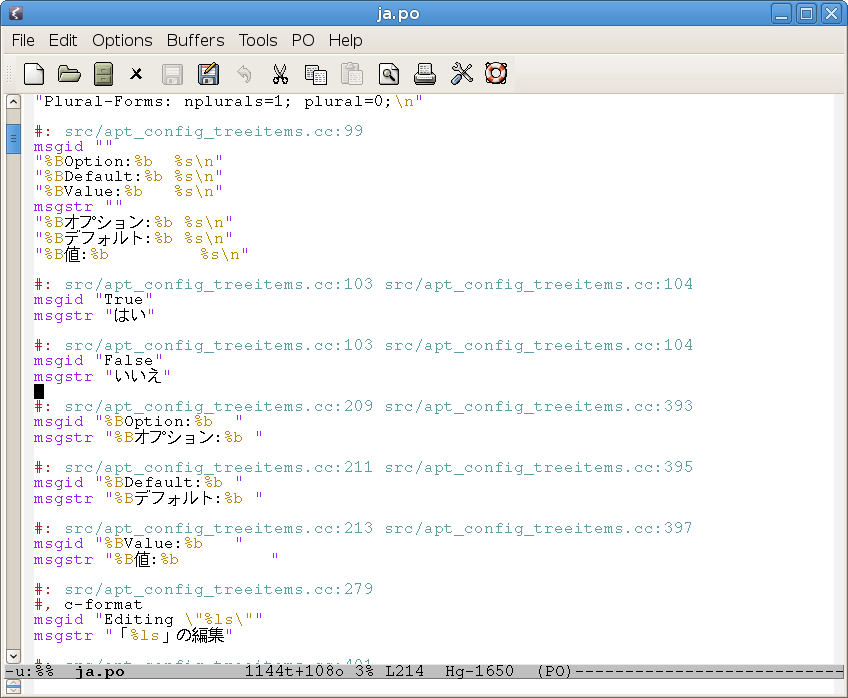
\includegraphics[width=0.4\hsize]{image200809/po-mode.png}
  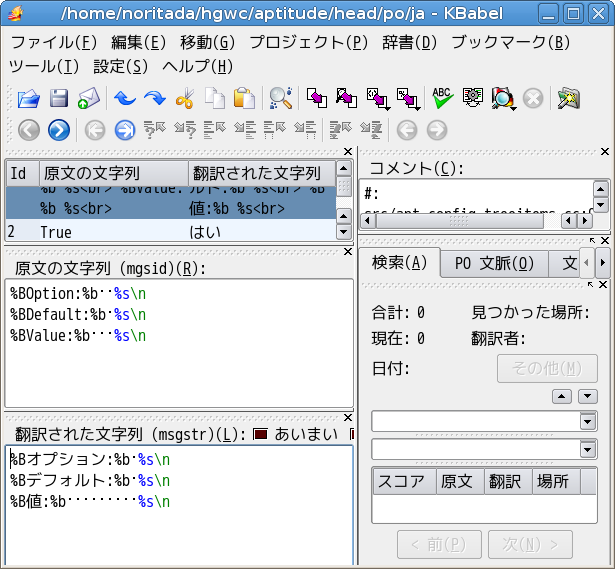
\includegraphics[width=0.4\hsize]{image200809/KBabel.png}
 \end{center}
 \caption{po-modeとKBabel}
 \label{fig:po-editors}
\end{figure}

以上の簡単な説明から分かると思いますが、po-modeは移動や編集がしやすく、
非常に便利です。

ただ、po-modeには今のところ翻訳メモリのような機能はありません。
KBabelやGtranslatorは翻訳メモリを備えているので、
翻訳メモリに興味のあるかたはこれらを試してみるのもよいでしょう。

\subsubsection{GNU gettextツール群}

翻訳作業にはPO編集ツールを使うことになるでしょうが、
一方でGNU gettextが提供する、
POやPOTに対してコマンドラインから自動処理できるツール群も、知っておくと便利です。
以下でざっと説明します。

\begin{description}
 \item[\texttt{msgattrib}] エントリの状態に応じた一括処理をします。
	    例えば、「fuzzyエントリのみにする」、「fuzzyエントリからfuzzyフラグを取り除く」といったことが可能です。
 \item[\texttt{msgcat}] 複数のPOを繋げます。
 \item[\texttt{msgcmp}] POとPOTが含む\texttt{msgid}セットを比較します。
 \item[\texttt{msgcomm}] 複数のPOに含まれる共通の\texttt{msgid}を抽出します。
 \item[\texttt{msgconv}] POの文字セットを変換します。
 \item[\texttt{msgen}] 英語のPOを作成します。
	    入力ファイルの未訳のエントリの\texttt{msgstr}に、\texttt{msgid}と同じ文字列を設定します。
 \item[\texttt{msgexec}] POに含まれるすべての翻訳に対してコマンドを実行します。
 \item[\texttt{msgfilter}] POに含まれるすべての翻訳に対して共通の処理をします。
 \item[\texttt{msgfmt}] POをコンパイルしてMOに変換します。
 \item[\texttt{msggrep}] パターンにマッチしたエントリをPOから抽出します。
 \item[\texttt{msginit}] POを初期化します。
 \item[\texttt{msgmerge}] POにPOTをマージします。
 \item[\texttt{msgunfmt}] MOからPOに逆コンパイルします。
 \item[\texttt{msguniq}] POに含まれる重複した\texttt{msgid}を1つにまとめます。
 \item[\texttt{xgettext}] ソースコードから\texttt{msgid}を抽出してPOTを生成します。
\end{description}

開発者が主に使うのは\texttt{xgettext}と\texttt{msgmerge}、\texttt{msgfmt}ですが、
他のツールも使いこなせるようになっておくと便利です。
使い方は各ツールのマニュアルページを参照してください。

\subsubsection{まとめ}

POはプログラム翻訳のために作られたファイル形式で、参照コメントのような翻訳に有用な情報や、
fuzzyエントリのような翻訳作業・保守作業の効率を上げるための仕組みを含んでいることを説明しました。
また、POという書式に特化した編集ツールについても説明しました。

\subsection{ドキュメント翻訳でPOを使うという考え方}

プログラム翻訳のために生み出されたPOは、
翻訳者にとって翻訳と保守の両方の作業をしやすい環境を提供する存在となりました。
その理由としては以下のようなものが考えられます。

\begin{itemize}
 \item PO自体に翻訳と保守を支援するための仕組みがある上、
       翻訳支援機能を持つPO編集ツールも存在する。
 \item メッセージの管理はツールがやってくれるので、人間は翻訳の管理に集中していればよい。
       \begin{itemize}
	\item メッセージがソースコードのどこにあるかが翻訳者にとって重要でないので、
	      メッセージがソースコード内で移動しても翻訳者は気にする必要がない。
	\item \texttt{msgmerge}でPOを更新すると、どのエントリの翻訳を更新すべきか瞬時に分かり、
	      PO編集ツールでそのエントリへ簡単に移動できる。
       \end{itemize}
\end{itemize}

一方でドキュメント翻訳については、通常は原文をそのままコピーして翻訳作業を開始するため、
翻訳以外の部分 (インデント、ドキュメント内での位置など) に変更があった場合、
その影響を翻訳者が受けます。
プログラム翻訳と比べて分量が多いのに保守性が低いので、
結果として翻訳者への負担は非常に大きくなります。
この状況は、翻訳者にとって大きな悩みの種でした。

そこで生まれたのが、ドキュメント翻訳に対してもPOを使おうという考え方です。
具体的には、ドキュメントの各ブロックをエントリとしたPOを作り、
ドキュメントとPOとを相互変換できるようにすることで、
翻訳者がPOでの翻訳管理に集中できるようにします。
以下のツールがそのような思想で作られています。

\begin{description}
 \item[Po4a] Debianで開発されている\footnote{厳密に書くと、Debian Project のメンバーが、
	    同プロジェクトが提供しているフリーソフトウェアプロジェクトホスティングサービスである Alioth 上で、
	    1つのプロジェクトとして開発しています。}。
	    対象とするドキュメント形式は、プレーンテキスト、XML、HTML、LaTeX、nroff (man)、Podなど多数で、
	    Perlで書かれたモジュールおよびプログラムの集合として実装されている。
	    Debianパッケージは\texttt{po4a}。
 \item[poxml] KDEで、KDE SDKモジュールの1つのコンポーネントとして開発されている。
	    対象とするドキュメント形式はDocBook XMLで、C++で実装された、
	    \texttt{po2xml}、\texttt{xml2pot}などの実行可能プログラムから成る。
	    Debianパッケージは\texttt{poxml}。
 \item[xml2po] GNOMEでgnome-doc-utilsの1つのユーティリティとして開発されている。
	    対象とするドキュメント形式はDocBook XMLである。
	    Pythonで実装されたシンプルな1つのファイルから成るので、
	    手軽にドキュメントのビルドに使用できる。
	    Debianでは\texttt{gnome-doc-utils}パッケージに含まれる。
\end{description}

poxmlやxml2poがDocBook XMLのみを扱うツールであるのに対し、
Po4aが様々な形式をサポートしているのは、
おそらくGNOMEやKDEとDebianの立場の違いを反映しているのでしょう。
GNOMEやKDEはプロジェクト内でドキュメント形式をDocBook XMLに統一できますが、
ディストリビュータであるDebianでは、
様々なソフトウェアの様々なドキュメントに対応する必要があるのです。

以降のセクションでは、ドキュメント翻訳にPOを使用する3つのツールのうち、
唯一複数のドキュメント形式をサポートしているPo4aについて見ていきます。

\subsection{Po4aの基本}

Po4aというソフトウェア名は、「po for anything」から来ています。
名前からも分かるように、
最初から様々なドキュメント形式の翻訳をPOで管理することを目的としており、
そのために入力形式として複数の形式を扱うことを想定した作りとなっています。

例えば、以下のような形式が現在サポートされています。

\begin{description}
 \item[KernelHelp] カーネル設定ヘルプのドキュメント形式です。
 \item[nroff] Unixの伝統あるマニュアルページの形式です。
	    BSDマニュアルページで使用されているmdoc形式もサポートされています。
	    初心者が読み書きしにくい形式ですが、
	    Po4aでサポートされたので、
	    インラインのマークアップだけ分かれば (原文の真似をすれば) 翻訳できます。
 \item[POD] Perl関連のドキュメントに使われる形式です。
	    ソースコードの横にコメントとして書き込まれたドキュメントは翻訳しにくいですが、
	    それをPOとして抽出し、翻訳しやすくします。
 \item[SGML] 最近ではXMLのほうが主流ですが、一昔前のドキュメント形式の主流です。
	    現在サポートされているDTDはDebianDoc-SGMLとDocBook SGMLのものです。
 \item[TeX/LaTeX] 著名な組版ソフトウェア\LaTeX{}の形式です。
 \item[GNU Texinfo] GNUのドキュメントに使用される形式です。
 \item[XML] 最近よく使われるドキュメント形式です。
	    現在サポートされているDTDはDia、DocBook XML、Guide XML、XHTMLのものです。
\end{description}

サポートされている形式の一覧は、
\texttt{po4a-gettextize}、\texttt{po4a-translate}、\texttt{po4a-updatepo}などのコマンドに\texttt{--help-format}オプションを与えると表示できます\footnote{残念ながら今のところ\texttt{po4a}コマンドに与えることはできないようです。}。
コマンドに\texttt{--format} (\texttt{-f}) などを与えてドキュメント形式を指定する場合、
この一覧に載っている名前を使用してください。

\begin{commandline}
noritada[3:39]%  po4a-gettextize --help-format   terra:~/svnwc/build-common/doc
有効フォーマット一覧:
  - dia: 非圧縮 Dia ダイアグラム。
  - docbook: Docbook XML。
  - guide: Gentoo Linux の xml ドキュメントフォーマット。
  - ini: .INI フォーマット。
  - kernelhelp: 各カーネルのコンパイルオプションのヘルプメッセージ。
  - latex: LaTeX フォーマット。
  - man: 古き良きマニュアルページフォーマット。
  - pod: Perl オンラインドキュメントフォーマット。
  - sgml: debiandoc と docbook DTD の双方。
  - texinfo: info ページフォーマット。
  - tex: 汎用 TeX ドキュメント (latex を参照)。
  - text: シンプルなテキストフォーマット。
  - wml: WML ドキュメント。
  - xhtml: XHTML ドキュメント。
  - xml: 汎用 XML ドキュメント (docbook を参照)。
\end{commandline}

\subsection{Po4aの使い方}

Po4aを用いた翻訳および翻訳更新手順について説明します。

まず、一から文書を翻訳する場合は以下のようになります。

\begin{itemize}
 \item 翻訳
       \begin{enumerate}
	\item 原文ドキュメント$\rightarrow$POT
	\item POT$\Rightarrow$PO [翻訳]
	\item PO$+$原文ドキュメント$\rightarrow$翻訳ドキュメント
       \end{enumerate}
 \item 翻訳更新
       \begin{enumerate}
	\item 原文ドキュメント (更新版)$\rightarrow$POT
	\item POT$+$PO (旧版)$\rightarrow$PO (エントリ更新版)
	\item PO (エントリ更新版) 翻訳更新
	\item PO (エントリ更新版)$+$原文ドキュメント (エントリ更新版)$\rightarrow$翻訳ドキュメント (エントリ更新版)
       \end{enumerate}
\end{itemize}

\subsubsection{導入(1): 原文ドキュメントファイルからPOTを生成する}

Po4aを使ってドキュメントの翻訳をする場合、最初にすべきことは、
原文のドキュメントファイルからPOTを生成することです。
POTの生成には\texttt{po4a-gettextize}コマンドを使用します。
\texttt{-f}オプションの引数にドキュメントファイルの形式を、
\texttt{-m}オプションの引数に原文ドキュメントファイル ({\bf マスタードキュメント}) の名前を、
\texttt{-p}オプションの引数に出力するPOTのファイル名を与えて、コマンドを実行します。
\texttt{-M}オプションの引数で、原文ドキュメントファイルの文字セットを指定することも可能です。

特に問題がない場合はすんなりとコマンドの実行が終了し、POTが生成されます。
ドキュメントの構造に問題がある場合 (例えばXMLにおいてタグがきちんと閉じられていない場合) はエラーになります。

POTが生成されたら、翻訳作業はプログラム翻訳の場合と同じです。
POTをコピーしてPOを作成し、ヘッダを適切に設定した上で翻訳作業を始めましょう。

\paragraph{例}
次の例では、\texttt{hoge.en.html}というXHTMLドキュメントから\texttt{hoge.pot}を生成しています。

\texttt{hoge.en.html} (入力):

\begin{commandline}
<?xml version="1.0" encoding="utf-8" ?>
<!DOCTYPE html PUBLIC "-//W3C//DTD XHTML 1.0 Strict//EN"
"http://www.w3.org/TR/xhtml1/DTD/xhtml1-strict.dtd">
<html xmlns="http://www.w3.org/1999/xhtml" lang="en" xml:lang="en">
<head>
<title>Test file</title>
</head>
<body>
<h1>Test file</h1>
<p>This is an <a href="apple">apple</a>.</p>
<p>This is an <a href="orange">orange</a>.</p>
</body>
</html>
\end{commandline}

コマンドライン:

\begin{commandline}
noritada[14:14]%  po4a-gettextize -v -f xhtml -m hoge.en.html -p hoge.pot    
\end{commandline}

\texttt{hoge.pot} (出力):

\begin{commandline}
# SOME DESCRIPTIVE TITLE
# Copyright (C) YEAR Free Software Foundation, Inc.
# This file is distributed under the same license as the PACKAGE package.
# FIRST AUTHOR <EMAIL@ADDRESS>, YEAR.
#
#, fuzzy
msgid ""
msgstr ""
"Project-Id-Version: PACKAGE VERSION\n"
"POT-Creation-Date: 2008-09-20 14:21+0900\n"
"PO-Revision-Date: YEAR-MO-DA HO:MI+ZONE\n"
"Last-Translator: FULL NAME <EMAIL@ADDRESS>\n"
"Language-Team: LANGUAGE <LL@li.org>\n"
"MIME-Version: 1.0\n"
"Content-Type: text/plain; charset=utf-8\n"
"Content-Transfer-Encoding: ENCODING"

# type: Attribute 'xml:lang' of: <html>
#: hoge.en.html:4 hoge.en.html:4
msgid "en"
msgstr ""

# type: Content of: <html><body><h1>
#: hoge.en.html:6 hoge.en.html:9
msgid "Test file"
msgstr ""

# type: Content of: <html><body><p>
#: hoge.en.html:10
msgid "This is an <a href=\"apple\">apple</a>."
msgstr ""

# type: Content of: <html><body><p>
#: hoge.en.html:11
msgid "This is an <a href=\"orange\">orange</a>."
msgstr ""
\end{commandline}

\subsubsection{導入(2): 原文・翻訳ドキュメントファイルからPOを生成する}

原文と同じ形式で翻訳したドキュメントが既にあり、
それをPo4a用のPOに移行したい場合にも、\texttt{po4a-gettextize}が使えます。
「POTをコピーしてPOを作った上で、
翻訳ドキュメントの各ブロックをコピー・アンド・ペーストでPOの各エントリに埋め込む」という、
間違いなくうんざりする作業は不要です。

ただしこの場合、どの原文がどの訳文に対応するかをPo4aが把握する必要があるので、
{\bf 原文ドキュメントファイルと翻訳ドキュメントファイルが同じ構造である}ことが前提になります。
「同じ構造」とは、Po4aが切り分ける単位、つまりブロックのレベルで見たときに、
対応する要素が同じ順序で並んでいる、という意味です。
もし翻訳側でブロックの追加や削除が行われていたら、変換はエラーで終わるでしょう。
一部のブロックの順序が入れ替わっている場合、変換は見た目は無事に終わるかもしれませんが、
入れ替わったブロックの\texttt{msgid}と\texttt{msgstr}の対応関係はおかしくなっているはずです。

訳注や翻訳者情報を別個のブロックとして翻訳ドキュメントに追加している場合、
それは一旦取り除いてください。
Po4aでは、POから翻訳ドキュメントを生成する際に、
原文にはない要素を追加する方法が提供されています。
方法については後述します。

原文ドキュメントファイルと翻訳ドキュメントファイルが同じ構造であれば、
\texttt{po4a-gettextize}を用いた変換は成功するはずです。
\texttt{-f}オプションの引数にドキュメントファイルの形式を、
POTを生成する場合の一連のオプションに加えて、
\texttt{-l}オプションの引数に翻訳ドキュメントファイルの名前を与えてコマンドを実行します。
\texttt{-L}オプションの引数で、翻訳ドキュメントファイルの文字セットを指定することも可能です。

変換に成功すると、すべてのエントリにfuzzyフラグが設定されたPOが生成されます。
すべてのエントリにfuzzyフラグが設定されるのは、
「ざっとでもいいので、ユーザには変換後にすべてのエントリの原文と訳文を確認してほしい」という開発者の意図を反映したものです
ユーザが自由に編集できる普通のドキュメントに少し制限を与えてPo4aの管理下に置く\footnote{例えば、「ブロックの順序など全体的な構造を原文に合わせる必要がある」、「原文の同じ内容のブロックには、同じ訳文を当てる必要がある」など。}際には、
何かしらの問題が発生している可能性があるのです。

\paragraph{例}
以下では、先程の\texttt{hoge.en.html}に対応する日本語訳\texttt{hoge.ja.html}をPOに変換することを試みます。

まずは、とりあえず\texttt{po4a-gettextize}を実行してみました。

\texttt{hoge.ja.html} (入力):

\begin{commandline}
<?xml version="1.0" encoding="utf-8" ?>
<!DOCTYPE html PUBLIC "-//W3C//DTD XHTML 1.0 Strict//EN"
"http://www.w3.org/TR/xhtml1/DTD/xhtml1-strict.dtd">
<html xmlns="http://www.w3.org/1999/xhtml" lang="ja" xml:lang="ja">
<head>
<title>テストファイル</title>
</head>
<body>
<h1>テスト用のファイル</h1>
<p>これは<a href="apple">リンゴ</a>です。</p>
<p>これは<a href="orange">オレンジ</a>です。</p>
<p>(訳注: オレンジはミカンとは違います。)</p>
</body>
</html>
\end{commandline}

コマンドライン:

\begin{commandline}
noritada[14:54]%  po4a-gettextize -v -f xhtml -m hoge.en.html -l hoge.ja.html -p ja.po
po4a gettextize: Original has less strings than the translation (6<7). Please 
               fix it by removing the extra entry from the translated file. You 
               may need an addendum (cf po4a(7)) to reput the chunk in place 
               after gettextization. A possible cause is that a text duplicated 
               in the original is not translated the same way each time. Remove 
               one of the translations, and you're fine.
po4a gettextization: Structure disparity between original and translated files:
msgid (at hoge.en.html:6 hoge.en.html:9) is of type 'Content of: 
<html><body><h1>' while
msgstr (at hoge.ja.html:6) is of type 'Content of: <html><head><title>'.
Original text: Test file
Translated text: テストファイル
(result so far dumped to gettextization.failed.po)
The gettextization failed (once again). Don't give up, gettextizing is a subtle 
art, but this is only needed once to convert a project to the gorgeous luxus 
offered by po4a to translators.
Please refer to the po4a(7) documentation, the section "HOWTO convert a 
pre-existing translation to po4a?" contains several hints to help you in your 
task
\end{commandline}

訳注を独立したパラグラフにしたためにPOへの変換が失敗したと考え、
訳注の行を削ってもう一度\texttt{po4a-gettextize}を実行してみます。
入力ファイルの内容は省略します。

コマンドライン:

\begin{commandline}
noritada[14:55]%  po4a-gettextize -v -f xhtml -m hoge.en.html -l hoge.ja.html -p ja.po
po4a gettextization: Structure disparity between original and translated files:
msgid (at hoge.en.html:6 hoge.en.html:9) is of type 'Content of: 
<html><body><h1>' while
msgstr (at hoge.ja.html:6) is of type 'Content of: <html><head><title>'.
Original text: Test file
Translated text: テストファイル
(result so far dumped to gettextization.failed.po)
The gettextization failed (once again). Don't give up, gettextizing is a subtle 
art, but this is only needed once to convert a project to the gorgeous luxus 
offered by po4a to translators.
Please refer to the po4a(7) documentation, the section "HOWTO convert a 
pre-existing translation to po4a?" contains several hints to help you in your 
task
\end{commandline}

なんだか変なエラーが出てしまっています。
どうも、\texttt{title}と\texttt{h1}の原文がともに「Test file」なのに、
一方の訳は「テストファイル」で、他方の訳が「テスト用のファイル」となっていることに原因があるようです。
そこで、両方の訳を統一して\texttt{po4a-gettextize}にかけると、変換に成功します。

\texttt{hoge.ja.html} (入力):

\begin{commandline}
<?xml version="1.0" encoding="utf-8" ?>
<!DOCTYPE html PUBLIC "-//W3C//DTD XHTML 1.0 Strict//EN"
"http://www.w3.org/TR/xhtml1/DTD/xhtml1-strict.dtd">
<html xmlns="http://www.w3.org/1999/xhtml" lang="ja" xml:lang="ja">
<head>
<title>テストファイル</title>
</head>
<body>
<h1>テストファイル</h1>
<p>これは<a href="apple">リンゴ</a>です。</p>
<p>これは<a href="orange">オレンジ</a>です。</p>
</body>
</html>
\end{commandline}

コマンドライン:

\begin{commandline}
noritada[15:07]%  po4a-gettextize -v -f xhtml -m hoge.en.html -l hoge.ja.html -p ja.po
\end{commandline}

\texttt{ja.po} (出力):

\begin{commandline}
# SOME DESCRIPTIVE TITLE
# Copyright (C) YEAR Free Software Foundation, Inc.
# This file is distributed under the same license as the PACKAGE package.
# FIRST AUTHOR <EMAIL@ADDRESS>, YEAR.
#
#, fuzzy
msgid ""
msgstr ""
"Project-Id-Version: PACKAGE VERSION\n"
"POT-Creation-Date: 2008-09-20 15:07+0900\n"
"PO-Revision-Date: YEAR-MO-DA HO:MI+ZONE\n"
"Last-Translator: FULL NAME <EMAIL@ADDRESS>\n"
"Language-Team: LANGUAGE <LL@li.org>\n"
"MIME-Version: 1.0\n"
"Content-Type: text/plain; charset=utf-8\n"
"Content-Transfer-Encoding: ENCODING"

# type: Attribute 'xml:lang' of: <html>
#: hoge.en.html:4 hoge.en.html:4
#, fuzzy
msgid "en"
msgstr "ja"

# type: Content of: <html><body><h1>
#: hoge.en.html:6 hoge.en.html:9
#, fuzzy
msgid "Test file"
msgstr "テストファイル"

# type: Content of: <html><body><p>
#: hoge.en.html:10
#, fuzzy
msgid "This is an <a href=\"apple\">apple</a>."
msgstr "これは<a href=\"apple\">リンゴ</a>です。"

# type: Content of: <html><body><p>
#: hoge.en.html:11
#, fuzzy
msgid "This is an <a href=\"orange\">orange</a>."
msgstr "これは<a href=\"orange\">オレンジ</a>です。"
\end{commandline}

\subsubsection{POと原文ドキュメントファイルから翻訳ドキュメントファイルを生成する}

さて、POを作ることが目的なのではありません。
当然ながらPOは翻訳を管理するための手段に過ぎません。
重要なのは、翻訳済みPOと原文ドキュメントから翻訳ドキュメントを出力することです。

\texttt{po4a-translate}

\subsubsection{原文ドキュメントファイルの更新をPOに反映させる}

\texttt{po4a-updatepo}

\subsubsection{POと翻訳ドキュメントファイルを一括更新する}

\texttt{po4a}

\subsubsection{原文にない要素を翻訳ドキュメントファイルに挿入する}

addenum

\dancersection{【でびあん】Debian パッケージメンテナというお仕事【現在募集中】}{やまね ひでき}

\label{sec:dm-yamane}
\index{Package maintainer}

\subsection{Debian パッケージメンテナのお仕事}

実は、Debian パッケージのメンテナになるにはそんなに敷居は高くありません。よっぽど入学試験/就職/転職活動の方が難しいと思うほどです。恐れることはありません。多少なりとも興味がある方はこれからの説明をご覧ください。

\subsection{メンテナになる前の下準備}

\begin{enumerate}
 \item GPG 鍵を作っておく (aptitude install gpg \&\& gpg --gen-key)\index{gpg}
 \item 公的な身分証明書を用意しておく
 \item 先ほど作った GPG 鍵と身分証明書を利用して、既存の Debian Developer とGPG キーサインの交換を行っておく
 \item メンテナや Developer として問題ないと見なされる作業をしておく (contribute!)
\end{enumerate}

この4つだけ準備したら、さぁ、メンテナになる作業の始まりです。


\subsection{The way to Debian package maintainer}

メンテナになる方法としては2点あります。

\begin{enumerate}
 \item 自分から「このソフトを Debian パッケージにしたい」と申請する
 \item 既存のパッケージのメンテナからメンテナンスを引き継ぐ
\end{enumerate}

1. は ITP (Intent To Package) という形で行います。特に RFP (Request For Package) という形でユーザから「このソフトを Debian パッケージにして欲しいなぁ」という声に答えるのが望ましいでしょう。\index{ITP}\index{RFP}

2. は RFH (Request For Help、協力者募集中)、RFA (Request for Adoption、新メンテナ募集中) や O (Orphaned、みなしご化) というステータスになったパッケージに対して「自分がメンテナになります」と宣言します。

ITP, RFP, RFA, Orphaned は全て Debian Bug Tracking System (BTS) で管理登録されます (BTS の使い方についてはそのうち別途)。これらを総称して「作業が望まれるパッケージ (Work-Needing and Prospective Packages; WNPP)」と呼びます。この WNPP、BTS で追うのは結構辛いので wnpp.debian.net \footnote{ \url{http://wnpp.debian.net} ではパッケージ化希望されているものや、メンテナが引き取り手を募集しているパッケージを検索できます。
\begin{itemize}
 \item ページの見た目は良くない ;-)
 \item RSSで状況が取得できるので、RSS reader で適宜ピックアップにてチェックすることをお勧めします。
\end{itemize}} を使いましょう。各略語の意味などについては \url{http://www.jp.debian.org/devel/wnpp/} をご覧ください。


\subsubsection{ITP、RFP パッケージ化}

大抵1からパッケージ化作業ですので、ウェブサイトからソースを取得してライセンスを確認の上、パッケージ作りのお作法に従ってパッケージを作成します。パッケージを作成する際は、unstable 環境の lintian で warning などが出なくなるよう (Debian Policy Manual に準拠するよう) に頑張りましょう。パッケージが作成できたら pbuilder でクリーンルーム環境でビルド可能かどうか (Build-Depends に間違いが無いか) のチェックを行います。問題なくビルドできたら piuparts を使ってインストール/アンインストールで問題が無いか (Depends や preinst, postinst, prerm, postrm スクリプトに問題が無いか) を確認しましょう。ここまで来て問題なければ「Eat your own dog food」、つまり自分の環境にパッケージを入れて問題が起きないかどうかチェックするとベストでしょう。
\index{pbuilder}

\begin{screen}
\paragraph*{ライセンスについて}
ちなみに一番大変なのはここでの「ライセンス確認」作業だと個人的には思っています。そのソフトのウェブページににちょっと書いてあることを鵜呑みにしたりすると、実は中身は全然違うライセンスだ、とか、実はリンクするライブラリとは矛盾するライセンスだ、とかがありますし、英訳ライセンスがないと Debian のパッケージ管理者 (ftpmaster) がライセンス的にそのパッケージを受け入れるかどうかの判断がそもそも出来ませんので必ず適当な英訳ライセンスへの翻訳作業が必要です。

ライセンスは、独自ライセンスよりも一般的に FLOSS の代表的ライセンス (GPL, BSD, MIT, Artistic など) を使う方が全ての利害関係者にとって利益があるでしょう。何故ならば、ライセンスは「プロトコル」のようなものであり、既存プロトコルを利用する方が新たにプロトコルを実装するよりもはるかに容易に取り扱えるからです。代表的ライセンスでは目的が達成できないときにのみ、独自ライセンスを利用するのが賢いやり方です。
\end{screen}

\subsubsection{RFA、Orphan への対処}

すでに現在のメンテナが引き継ぎ手を募集している状態 (RFA) や、完全にギブアップor興味を失ってしまった (Orphan) パッケージについては、BTS を利用してパッケージを引き取る旨の宣言 (ITA, Intend To Adapt) を行いましょう。加えて関連のメーリングリストで「自分がやろうと思うけど、どう?」と聞いてみるとさらに良いでしょう。合意がとれたら、debian/changelog にて該当の RFA/Orphan バグを閉じるエントリを追記しておきます。大抵の場合は色々とバグレポートが溜まっているので片付けて同様に changelog に記載しておきましょう。


\subsection{アップロード}

ここまでが終わったらアップロードを行います。Debian Developer であればパッケージを dput や dupload と呼ばれるコマンドを使って、作成されたソースパッケージとバイナリパッケージを直接 Debian へアップロードします。そうでない場合は適当な場所にアップロードして、Debian Developer に代理アップロードをお願いしましょう (アップロード先は、\url{http:://mentors.debian.net}、代理アップロード依頼先は \url{debian-devel@debian.or.jp} がおすすめです)。 

\begin{commandline}
dupload -t anonymous-ftp-master ccspatch_1.6.4-20080903-1_i386.changes
\end{commandline}

この時点でツールは \texttt{.dsc} ファイルや \texttt{.changes} ファイルに gpg 署名されているかどうかをチェックして、されていない場合はアップロードしないなどしてくれます。

サーバ側では、まず「既にあるパッケージの更新なのか、それとも新規パッケージなのか」の判断を行います。新規パッケージの場合は NEW Queue \footnote{\url{http://ftp-master.debian.org/new.html}} と呼ばれる所に自動的に移されて、ftpmaster が逐次入れてよいものかどうかのチェックを行っています。おおよそこの工程は1、2週間程度かかります。

チェックは特にライセンスの問題が無いかについてなどが争点となります。この作業は高度な判断が要求されるため、人的リソース的にボトルネックになりやすいところと、拒否された場合に「何故このパッケージが拒否されたのか」の記録が容易にトラッキングできないのが問題点です。人的リソースについては、アクティブなメンバーを入れることで以前と比較しても改善がされており、トラッキングについては最近になってシステマチックにチェック可能なように提案が出てきているところです。

更新パッケージについては、サーバ側でソースパッケージの gpg 署名をチェックなどをして「本当にこれは入れていいものかどうか」を判断してダメな場合は reject されます。このチェックについては、アップロード後にサーバから受け入れ/拒否のメールが届きます。

まずアップロードされたパッケージの処理を始めたよ、というメール

\begin{commandline}
From: Archive Administrator <dak@ftp-master.debian.org>
Subject: Processing of ccspatch_1.6.4-20080903-1_i386.changes

ccspatch_1.6.4-20080903-1_i386.changes uploaded successfully to localhost
along with the files:
  ccspatch_1.6.4-20080903-1.dsc
  ccspatch_1.6.4-20080903.orig.tar.gz
  ccspatch_1.6.4-20080903-1.diff.gz
  linux-patch-tomoyo_1.6.4-20080903-1_all.deb

Greetings,

	Your Debian queue daemon
\end{commandline}


チェックして incoming repository に入れたよ、というメール

\begin{commandline}
From: Debian Installer <installer@ftp-master.debian.org>
Subject: ccspatch_1.6.4-20080903-1_i386.changes ACCEPTED

Accepted:
ccspatch_1.6.4-20080903-1.diff.gz
  to pool/main/c/ccspatch/ccspatch_1.6.4-20080903-1.diff.gz
ccspatch_1.6.4-20080903-1.dsc
  to pool/main/c/ccspatch/ccspatch_1.6.4-20080903-1.dsc
ccspatch_1.6.4-20080903.orig.tar.gz
  to pool/main/c/ccspatch/ccspatch_1.6.4-20080903.orig.tar.gz
linux-patch-tomoyo_1.6.4-20080903-1_all.deb
  to pool/main/c/ccspatch/linux-patch-tomoyo_1.6.4-20080903-1_all.deb


Override entries for your package:
ccspatch_1.6.4-20080903-1.dsc - source devel
linux-patch-tomoyo_1.6.4-20080903-1_all.deb - extra admin

Announcing to debian-devel-changes@lists.debian.org


Thank you for your contribution to Debian.
\end{commandline}

これでパッケージのアップロードが完了しました。BTS に記載されているバグを修正した旨を debian/changelog に適切なスタイルで記述しておくと、BTS から bug closed のメールがやってきます。


\subsubsection{その他アップロードに関する注意}

ちなみに、Debian バージョンのみの更新の場合 (foo 1.0-1 から foo 1.0-2 への更新など) はオリジナルのソースファイル (orig.tar.gz) をアップロードしないことになっています。もし、orig.tar.gz をアップロードした場合は後から拒否のメールが届きます。

あと注意として、ライブラリファイルや他の多くのパッケージと関連しているようなパッケージで更新をかけると unstable 環境が壊れるような場合は、experimental へアップロードして関係者と調整することが推奨されています。


\subsection{メンテナンス作業}

BTS を通じてユーザからバグ報告メールが来るので、それに対応してパッケージの debian ディレクトリ以下を更新して、修正出来たら changelog に完了した旨を記載しておきます (dch コマンドが便利です)。特に RC (Release Critical) バグは早めに修正しましょう。バグが他のパッケージと関連する場合は適当なメーリングリストで関係者と対応を協議して進めていきます。場合によっては、自分のパッケージのバグではなく、他のパッケージのバグである場合もありますので、その場合はバグを BTS で reassign しておきます。パッケージとしてのバグではなく、元々のソース由来のバグの場合は、バグを upstream (開発元) に転送するかパッチを作って upstream と協議しましょう。

そして upstream での更新に合わせてパッケージも更新します。upstream の更新は debian/watch ファイルを適切に記載していれば、DEHS \footnote{Debian External Health Status\url{http://dehs.alioth.debian.org}} によって定期的にチェックされ、Debian Quality Assuarance の developer ページ \footnote{\url{http://qa.debian.org/developer.php}} で状況を確認できます (あとは upstream のリリースアナウンスが流れるメーリングリストに入っておくと良いでしょう)。きちんと設定された \texttt{debian/watch} ファイルがあれば、パッケージによっては更新がものの1分も経たずに出来ます。

チーム制でメンテナンスをするような場合は共有 repository に更新したソースを忘れずに commit しておきましょう。commit 出来ない場合は、チームのメーリングリストにパッチを送ります。幾度か適切なパッチを送りつづけていると、いつの間にか commit 権が与えられていることが多い様です。

なお、バグ修正や Debian Policy に適合するために Debian パッケージ側で色々とパッチを当てている (dpatch や quilt を利用する) と新バージョン側のソースとコンフリクトを起こしてその修正に時間がかかることがありますので、なるべく upstream の開発者とメーリングリストなどを通じて普段からコンタクトを取り合っておいて、パッチ自体が取り込まれて不要になるように働きかけましょう。

この様にしてパッケージ化、メンテナンス等をメンテナは日々行っていきます。特に問題なく時間が経過したパッケージは unstable から testing に移行され、次のリリースを待つことになります。そして、リリースの日を迎えたパッケージは stable へと移されます。


\subsection{特殊な場合}

以下に頻繁には起きないはずの、ちょっと変わった場合の対応を挙げておきます。

\subsubsection{NMU}

Non-Maintainer Upload の略で、既存のメンテナ以外の人間がバグ修正のためにパッケージをアップロードすることを指します。あまり頻繁に NMU があるようなパッケージについては、メンテナが本当に活動しているのかどうかをチェックした方がいいでしょう。

\subsubsection{FREEEEEEZE!!}

 特にリリース前には「システム全体の安定化」が必要なため、freeze、つまりパッケージの unstable から testing への自動移行が停止されます。しかし、freeze の間に発覚した、そのままリリースされてしまっては困るようなバグの修正が必要な場合もあります。その場合は リリースマネージャ (RM) に対して「私のこのパッケージを testing に入れるようにしてください!」とお願いします。これを「unblock (exception) request」と一般に呼びます。やり方としてはメーリングリストで RM が理解しやすいフォーマットでメールを投げるだけです。

\begin{commandline}
To: debian-release@lists.debian.org
subject: Please unblock <package> <version>
\end{commandline}

\begin{itemize}
 \item changelog の抜粋
 \item 理由
 \item debian-devel-announce で流れている freeze exception のどれに当てはまるのか
 \item このアップデートによって何が改善されるのか
 \item このアップデートでは regression が起きない説明
 \item その他、RM が納得してくれるような内容
\end{itemize}

うまくすれば RM から "unblocked" という素っ気ないメールが届きます。これが来たら大成功です。今 unstable にあるパッケージは testing へ移行することが可能になります。


\subsection{メンテナ権の移譲}

パッケージメンテナも人の子、残念ながら諸事情によりメンテナンスが出来なくなるような事態が起きるかもしれません。なるべく一人でメンテナンスせずチームあるいは自分以外の詳しい/信用できるメンテナもアップロードできるようにしておきます。具体的には debian/control の Uploaders フィールドにアップロードしてもいい人の名前とメールアドレスを書いておきます (GPG 署名に使うものと同一である必要があります)。

\begin{commandline}
Source: ttf-vlgothic
Section: x11
Priority: optional
Maintainer: Debian Fonts Task Force <pkg-fonts-devel@lists.alioth.debian.org>
Uploaders: Hideki Yamane (Debian-JP) <henrich@debian.or.jp>
DM-Upload-Allowed: yes
Build-Depends: debhelper (>= 5)
Build-Depends-Indep: defoma, bzip2
Standards-Version: 3.8.0
Homepage: http://dicey.org/vlgothic/
Vcs-Svn: svn://svn.debian.org/pkg-fonts/packages/ttf-vlgothic/
Vcs-Browser: http://svn.debian.org/wsvn/pkg-fonts/packages/ttf-vlgothic/
\end{commandline}

そして、メンテナンスが出来なくなりそうな場合は、あまり粘らずにさっさと
宣言 (RFA、Orphan) しておきましょう。宣言が無いと「このパッケージ古いな」という悪評が立つだけ…という結果になりかねません。なお、日本の首相と違ってメンテナは頻繁に交代してもきちんとした理由があれば文句は言われることはありません :-) (できれば最初の方から複数人でのチームメンテナンスなどしておくと困ったことになる確率は減ります)


\subsection{終わりに}
如何でしたか?パッケージメンテナというお仕事がどのようなものか、多少理解が深まっていただければ幸いです。


% tokyoresume200810 / 45
% -- OSC 2008 Tokyo Fall

% tokyoresume200811 / 46 

\dancersection{Debconf8 参加報告}{上川 純一}
\label{sec:debconf8uekawa}
\index{debconf8}
\index{Debian Conference 2008}

\subsection{Debconfとは}

2008年度の Debconf は 8月10日から8月16日まで、アルゼンチンのマルデル
プラタで行われました。日本からは、上川 純一が参加しました。

\subsubsection{Debconfの歴史・経緯}

Debian Conference \footnote{\url{http://debconf8.debconf.org/}}は Debian 
の開発者たちが一堂に会するイベントです。通常顔をあわせることのないメンバー
たちが一堂に会し友好を深め、技術的な議論を戦わせます。過去の開催履歴を見
てみると\tbref{tab:debconflist8}のようになります。

\begin{table}[H]
\caption{歴代のDebconf参加者推移}
\label{tab:debconflist8}
 \begin{center}
 {\footnotesize
 \begin{tabular}{|c|c|c|r|}
 \hline
 年 & 名前 & 場所 & 参加人数 \\
 \hline
 2000 & debconf 0 &フランス ボルドー & \\
 2001 & debconf 1 &フランス ボルドー & \\
 2002 & debconf 2 &カナダ トロント & 90名 \\
 2003 & debconf 3 &ノルウェー オスロ & 140名 \\
 2004 & debconf 4 &ブラジル ポルトアレグレ &  150名 \\
 2005 & debconf 5 &フィンランド ヘルシンキ & 200名 \\
 2006 & debconf 6 &メキシコ オアスタペック & 300名 \\
 2007 & debconf 7 &英国スコットランド エジンバラ & 約400名 \\
 2008 & debconf 8 &アルゼンチン マルデルプラタ & 約200名 \\
 \hline
 \end{tabular}
 }
 \end{center}
\end{table}

\subsubsection{Debconf 2008} 2008年度の Debconf は海辺のホテルを二棟借
りて開催しました。宿泊しているホテルの7Fと1Fがハックラボになっており、
7Fがカンファレンスルームになっているという便利な環境でした。

\subsection{アルゼンチン・マルデルプラタ}

\subsubsection{行き方}
  日本からアルゼンチンまでは、直行便がありません。
  上川はサンフランシスコ・カナダのトロント・チリのサンチャゴを経由して
  アルゼンチンのブエノスアイレスまで移動(ここまでで約30時間程度)、
  そこからバスで移動(5時間(直行)から10時間(乗り換え))しました。

  今回の会期は従来と違い長期休暇でバカンスをとっている人の多い時期です。
そのため、飛行機の予約のタイミングが難しかったかもしれません。
また、日本からアルゼンチンにいく便には安いものがあまりみつからず苦労しました。

ブエノスアイレスからマルデルプラタの間は東京・大阪間程度の距離があり、
多数のバスが通っています。空港からブエノスアイレスの市街で乗り換えれば多数のバスがあるのですが、
空港からの直行のバスは非常に少なく(Manuel Tenda Leonという会社のバスのみが運行している模様)、
予約ができない人がでていたようです。

\subsubsection{会場}

\begin{wrapfigure}{r}{6cm}
  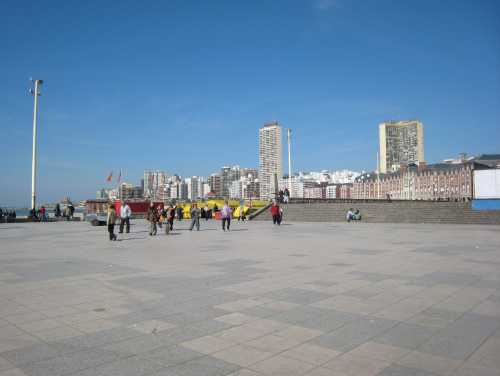
\includegraphics[width=\hsize]{image200810/mdq-area.jpg}
\end{wrapfigure}
会場はビーチリゾートとして知られるマルデルプラタの中央カジノ前のホテルでした。
\\


\subsection{スケジュール}

8月10日から開始し、8月16日までイベントがぎっしりつまっていました。
8月18日にブエノスアイレスに移動し、そこでDebian Day を開催しました。

\subsection{会期中で気になったこと}

上川が今回参加して気になったことを紹介します。

Debconf に参加しているミラーサーバはフルミラーではなくアーキテクチャ
i386、 amd64、 ppc と armel でした。

qemubuilder を開発している関係でarmel関連の作業を行いました。
qemubuilder の armel 移植と、armel 関連のデバッグなどです。
しかしながら途中でPCのHDDが故障し後半はHDDの購入からインストール、
macbookのブートローダのデバッグに費しました。

PGPキーをICカードで利用する仕組みがあるみたいで、作成していました。
ただ、仕組みがよくわからないので今回はスルーしました。

%
\dancersection{「その場で勉強会資料を作成しちゃえ」 Debian を使った \LaTeX 原稿作成合宿}{上川 純一}
\label{sec:latexdebmtgres}
\index{latex}

\subsection{概要}

Debian 勉強会では資料を \LaTeX で管理しています。
Emacs、 Git、 \LaTeX で Debian 勉強会資料作成をする流れを体験してみましょう。
\index{emacs}
\index{platex}

ハンズオンでDebian 勉強会資料のチェックアウト、作成からコミットまでの流れ
を一通り試します。途中でつまったらできるまで現地で対応する予定です。
\footnote{ベストエフォート、もしかするとできない場合もあります}。

\subsection{事前準備}

当日の時間は限られているため、事前準備が必要です。
現地に入るまでに準備しておくものです

\begin{itemize}
 \item 無線LAN接続可能なノートパソコン
       (十分長いLANケーブルを持参しても可能、スイッチも持参してください)
 \item 必要なパッケージをインストールした Debian GNU/Linux sid のシステ
       ム
 \item 記事にする内容。
       紹介したいツール/パッケージ関連のコマンドライン出力と
       画面写真と簡単な説明文章。
\end{itemize}

事前にインストールしておいて欲しい必要なパッケージは

\begin{itemize}
 \item 基本ツール: make 
 \item \LaTeX 一式: ptex-bin dvipdfmx latex-beamer  okumura-clsfiles
       ghostscript-x\footnote{lenny以前での gs-esp 相当} xpdf 
       xpdf-japanese evince poppler-data texlive-latex-extra
 \item emacs / whizzytex 関連一式: whizzytex advi
       emacs22-gtk\footnote{emacs22 でもよい、emacs22-nox は難しいかも} 
       yatex gs-cjk-resource gv
 \item Git 関連一式: git-core git-gui qgit
 \item DHCP / Avahi 関連一式: avahi-daemon avahi-autoipd libnss-mdns
 \item 日本語フォント関連: ttf-mona ttf-sazanami-mincho ttf-vlgothic
 \item 日本語入力関連: scim-anthy 
\end{itemize}
\index{whizzytex}
\index{Active DVI}
\index{avahi}

avahi の設定が正しいことは、ping ホスト名.local が使えるかどうかで確認し
ます。/etc/nsswitch.conf の hosts 行にmdns\footnote{なんらかの mdns の設
定であればよく、例えば mdns4 であってもよい。}を参照する設定が追加されている
ことを確認してください。

\begin{commandline}
hosts:          files mdns dns
\end{commandline}

% 実験的には念のため apt-get には -o APT::Install-Recommends=false を指定
% して確認している。 

\begin{commandline}
# apt-get update
# apt-get install \
 make ptex-bin dvipdfmx latex-beamer \
 okumura-clsfiles ghostscript-x xpdf xpdf-japanese whizzytex \
 evince poppler-data \
 texlive-latex-extra \
 advi emacs22-gtk yatex gs-cjk-resource gv git-core git-gui \
 qgit avahi-daemon \
 libnss-mdns avahi-autoipd \
 ttf-mona ttf-sazanami-mincho ttf-vlgothic \
 scim-anthy
# jisftconfig add
\end{commandline}
\footnote{okumura-clsfiles の依存する ptex-jisfonts はインストール後に手
動で設定をする必要がある。
具体的には jisftconfig add を実行。}

事前にダウンロードしてビルドできる環境であることを確認しておいてください。

\begin{commandline}
$ git clone git://git.debian.org/git/tokyodebian/monthly-report.git
$ cd monthly-report
$ cp -p git-pre-commit.sh .git/hooks/pre-commit
$ make -j4 
$ ls *.pdf # 110くらいのPDFファイルが生成されていることを確認
\end{commandline}

Emacs の設定をします。
yatex の設定と
文字コードの設定をします。

.emacs に

\begin{commandline}
;; YaTeX が漢字コードを毎回ISO-2022-JPに設定しないようにする
(setq YaTeX-kanji-code nil)

;; git.el をロードする
(load-library "/usr/share/doc/git-core/contrib/emacs/git.el")
\end{commandline}

Git の設定もしておきましょう。
ユーザ名とメールアドレスを設定します。
設定しないとホスト名や /etc/passwd の設定をデフォルトで使ってしまいます。

\begin{commandline}
$ git config --global user.email dancer@netfort.gr.jp
$ git config --global user.name "Junichi Uekawa"
\end{commandline}

\subsection{演習0: 環境設定}

勉強会の会場で準備している環境です

\begin{itemize}
 \item avahi 経由で接続できる Debian package cache (i386、amd64)
 \item 無線LAN(WEP) ESSID:会場にて発表
\end{itemize}

DHCPでネットワーク接続してください。
avahi(mDNS) で名前解決できることを確認してください。
apt リポジトリの設定が可能であることを確認してください。


\begin{commandline}
# ping coreduo.local
# cat /etc/apt/sources.list
deb http://coreduo.local:9999/debian/ sid main contrib non-free
# apt-get update 
\end{commandline}


\subsection{演習1: リポジトリチェックアウト}

\begin{commandline}
$ git clone git://coreduo.local/git/monthly-report.git
\end{commandline}

\begin{commandline}
$ make -j4 # エラーがでます
$ cp -p git-pre-commit.sh .git/hooks/pre-commit
$ make -j4
\end{commandline}


\subsection{演習2: emacs whizzytex 起動}

\begin{commandline}
$ cd XXXXX
$ emacs
\end{commandline}

whizzytexを起動します。
プリビューが開始するというメリットだけでなく、即時コンパイルエラーを検出
できるのが重要です。

\begin{commandline}
M-x whizzytex-mode 
\end{commandline}

スペルチェックも起動しましょう。\footnote{iamerican もしくは ibritish パッ
ケージが必要です。}

\begin{commandline}
M-x flyspell-mode
\end{commandline}

\subsection{演習3: セクションを追加}

まずセクションを追加します。

\begin{commandline}
 \dancersection{XXXX}{名前}
 \index{XXXX@YYYY}
 \label{XXXX@YYYY}

 % 本文

\end{commandline}

\subsection{演習4: 説明の章だてを書いてみる}

\begin{commandline}

\subsection{xxxx}

\subsection{xxxx}

\subsection{xxxx}

\subsection{xxxx}

\subsection{xxxx}

\end{commandline}

\subsection{演習5: 説明の中身を書いてみる}

文章は空行区切りでパラグラフになります。roffなどと同じです。
改行は無視されます。

\verb!\!ではじまる文字列が命令です
\begin{commandline}
 \XXXX{YYYY}
\end{commandline}

monthlyreport.sty で追加のコマンドが定義されています。
\footnote{フットノートが追加できます}

表を作ってみましょう。

\begin{table}[h]
\caption{キャプション}
\label{tab:1234}

 \begin{tabular}{|c|c|c|}
 \hline
 ディストリビューション & バージョン & 備考 \\
 \hline
 ディストリビューション & バージョン & 備考 \\
 ディストリビューション & バージョン & 備考 \\
 \hline
 \end{tabular}
\end{table}


知っておきたい構文は実はあまりたくさんはありません。
利用されている上位:

\begin{commandline}
$ sed -n 's/.*\(\\[a-z]\+\).*/\1/pg' *.tex  | sort | uniq -c | sort -rn  
   6948 \item
   6240 \end
   5628 \begin
   1952 \subsection
   1623 \subsubsection
   1491 \santaku
   1258 \url
   1189 \hsize
    895 \hline
    874 \texttt
    522 \dancersection
    473 \footnote
    451 \includegraphics
    447 \vspace
    405 \label
    378 \frametitle
    357 \usepackage
    323 \hspace
    316 \hrule
    300 \section
    253 \bf
    236 \index
\end{commandline}

利用されている上位の begin-end 構文

\begin{commandline}
$ sed -n 's/.*\(\\begin{[a-z]\+\).*/\1/pg' *.tex  | sort | uniq -c | sort -rn 
   1742 \begin{itemize
   1293 \begin{commandline
   1245 \begin{frame
    781 \begin{minipage
    271 \begin{center
    194 \begin{enumerate
    148 \begin{tabular
    133 \begin{figure
\end{commandline}

\newcommand{\debiangnulinux}{Debian GNU/Linux}

\debiangnulinux{}のようによく使う文字列はnewcommandで定義できます。
ただし、命令がファイル毎に別の意味を持つようになると
管理がしにくくなるのでできるだけ monthlyreport.sty に定義は集中させています。
monthlyreport.sty は共有しているので変更する際には御注意を。最初は変更内容につ
いて誰かにレビューをお願いしたほうがよいと思います。

\begin{commandline}
$ git log --pretty=format:%an monthlyreport.sty | sort | uniq -c 
     15 Junichi Uekawa
      3 Nobuhiro Iwamatsu
\end{commandline}

エスケープが必要な文字列の出力方法
\begin{itemize}
 \item \verb!\! verb は見にくくなるので最終的手段
 \item \~{}
 \item \^{}
 \item aaaa$<$aaaa そのままだと:<
 \item aaaa$>$aaaa そのままだと:>
 \item aaaa\#aaaa
 \item aaaa\%aaaa
 \item \_{}aaaa
\end{itemize}

よく使うコマンド
\begin{itemize}
 \item begin itemize / item / end itemize
 \item begin enumerate / item / end enumerate
 \item commandline (勉強会用に定義)
 \item includegraphics 後述
\end{itemize}

\subsection{演習6: コマンドライン出力を追加してみる}

\begin{commandline}
\ begin{commandline}

コマンドライン出力

\ end{commandline}
\end{commandline}

\subsection{演習7: png 画像を挿入してみる}

includegraphics

png 

git add

ebb

make で確認。

\subsection{演習8: git で変更をコミットしてみる}

\begin{commandline}
$ make 
\end{commandline}

\begin{commandline}
M-x git-status
\end{commandline}

\subsection{演習9: git での変更を送信してみる}

\begin{commandline}
$ git pull
\end{commandline}

コンフリクトを解消します。

\begin{commandline}
M-x git-status
\end{commandline}

\begin{commandline}
$ git push
\end{commandline}

\begin{commandline}
$ mkdir ~/patches/
$ git format-patch -o ~/patches/ HEAD^ 
\end{commandline}
生成されたパッチファイルをメールで送付します。

\subsection{演習10: git で変更をマージしてみる}

\subsection{演習11: 全体を眺める}

outline-minor-mode が便利です。


\subsection{今回演習できないTIPS}

\subsubsection{alioth tips}
資料の編集には alioth を利用します。
\url{alioth.debian.org}、 \url{git.debian.org} です。

Alioth にアカウントを作成します。
Debian Developer でない場合のユーザ名は、
XXXX-guestというユーザ名になります。

便利につかうため、\texttt{.ssh/config} に設定を追加しましょう。

\begin{commandline}
ServerAliveInterval 10
ServerAliveCountMax 12

Host alioth.debian.org
 ControlMaster auto
 ControlPath ~/tmp/ssh-%r@%h:%p
 User xxxx-guest

Host git.debian.org
 ControlMaster auto
 ControlPath ~/tmp/ssh-%r@%h:%p
 User xxxx-guest

Host localhost
 StrictHostKeyChecking no

Host *.local
  CheckHostIP no
\end{commandline}

% #### kansai ####
% kansairesume200808
\dancersection{DebianをWindowsなPCでも楽しもう --応用編}{名村 知弘}
\label{sec:colinux}
\index{coLinux}

\subsection{はじめに}
coLinuxの配布サイト
\footnote{\url{http://sourceforge.net/projects/colinux/files}}では、
Debian etchのイメージファイルが配布されていますので、
coLinuxをインストールすると、すぐにDebianを楽しむことができます。

しかし、配布されているイメージファイルは、
ディスクイメージのサイズが1GBだったり、
どのようなパッケージがどういった設定でセットアップされているのかなど、
中身が非常に気になったりします。

ダウンロードすればお手軽に使えるというのは良いのですが、
将来の拡張のためパーティション構成を変更したり、
イメージの内容をいちいち確認するのも面倒ですし、
それならばいっその事、新規インストールしてみよう。
と言うことで、半ば強引な導入ですが、
coLinuxにDebianを新規インストールする方法と、
coLinuxにインストールされたXアプリケーションを起動する方法をご紹介します。

説明するにあたり、以下の前提で記載していますので、
適宜それぞれの環境に応じて読み替えていただくようお願いいたします。
\begin{enumerate}
\item coLinuxを\verb|c:\coLinux|にインストールしているものとしています。
\item coLinuxはネットワーク共有にて接続されているものとしてます。
\item Debianはetchを使用するものとしています。
\item DebianはIPアドレス192.168.0.10が割り当てられているものとしています。
\end{enumerate}

\subsection{coLinuxにDebianを新規インストール}
coLinuxへのDebianインストール手順は以下のようになります。
\begin{enumerate}
\item Debianをインストールするためのディスクイメージの作成
\item DebianのISOイメージを入手
\item initrdイメージの取得
\item coLinuxをDebianインストール用に設定
\item Debianのインストール
\item coLinuxを通常起動用に設定
\end{enumerate}



\subsubsection{Debianをインストールするためのディスクイメージの作成}
coLinuxでは、1つのパーティションに対して1つのディスクイメージファイルを用意することで、
HDDをエミュレートしています。
ディスクイメージファイルはあらかじめ必要なサイズを割り当てる必要があり、
coLinuxが割り当てられたサイズを超えて書き込むことはできません。
(つまり、HDDが一杯になったら書き込めないのと同様、
ディスクイメージファイルに割り当てられたサイズを使用すると、それ以上書き込みが行えなくなります)

今回は以下の構成でインストールを行いたいと思います。
\begin{table}[htbp]
\begin{center}
  \begin{tabular}[htbp]{|l|l|l|}\hline
    領域 & サイズ & ディスクイメージ\\ \hline\hline
    / & 2GB & \verb|root_fs|\\ \hline
    /home & 2GB & \verb|home_fs|\\ \hline
    swap & 500MB & \verb|swap_fs|\\ \hline
  \end{tabular}
  \caption{パーティション割り当て}
  \label{tab:colinux_partition}
\end{center}
\end{table}

ここでは3パーティション使用するため、3ファイル作成する必要があります。
また、あらかじめ使用するサイズを割り当てる必要があるため、
Windowsのfsutilコマンドを使用します。
fsutilは指定されたファイル名、サイズで空ファイルを作成することができます。

ファイル名とサイズは表\ref{tab:colinux_partition}に基づいて決定していますので、
お手持ちのPCのディスク空き容量などを考慮しながら、
適切なサイズを決定していただければと思います。

コマンドプロンプトを起動し、\verb|c:\coLinux|にcdしてから、
以下のコマンドを実行するとファイルが作成されます。

\begin{commandline}
fsutil file createnew root_fs 2147483648
fsutil file createnew home_fs 2147483648
fsutil file createnew swap_fs 536870912
\end{commandline}

\subsubsection{DebianのISOイメージを入手}
まずはDebianをインストールするための、ISOイメージを入手
\footnote{\url{http://www.debian.org/CD/netinst/}}します。
ここではdebian-40r4a-i386-businesscard.isoを使用します。

\subsubsection{initrdイメージの取得}
\verb|c:\coLinux|には、
coLinux起動用のinitrdイメージが用意されていますが、
Debianインストール用にcoLinuxを起動するためには、
インストール用に起動するためのinitrdイメージが必要となります。

インストール起動用と通常起動用のinitrdイメージを混同してしまわないように、
\verb|c:\coLinux|にあるオリジナルのinitrd.gzを、
initrd-normal.gzとリネームしておきます。

インストール用のinitrdイメージは、DebianのISOイメージに収録されているため、
ISOイメージを展開できるツール、Explzh\footnote{\url{http://www.ponsoftware.com/archiver/}}や、
TUGZip\footnote{\url{http://www.tugzip.com/}}を使用して取り出します。

展開ツールをインストールして起動し、DebianのISOイメージを開きます。
ISOイメージの中の、「/install.386/initrd.gz」を取り出し、
こちらも通常起動用のinitrdイメージと混同してしまわないように、
initrd-install.gzとリネームして、\verb|c:\coLinux|に保存します。


\subsubsection{coLinuxをDebianインストール用に設定}
coLinuxをインストール用に起動するためのファイルは全て揃いましたので、
これらファイルを使用してDebianインストールが行われるよう、
coLinuxの設定を変更します。

\verb|c:\coLinux|にdebian-install.confと言う名前でファイルを作成し、
以下の内容を記載して保存します。

\begin{commandline}
kernel=vmlinux
initrd=initrd-install.gz
mem=512
cobd0="\DosDevices\C:\coLinux\swap_fs"
cobd1="\DosDevices\C:\coLinux\root_fs"
cobd2="\DosDevices\C:\coLinux\home_fs"
cobd3="\DosDevices\C:\coLinux\debian-40r4a-i386-businesscard.iso"
cofs0="\DosDevices\C:\coLinux"
eth0=tuntap
root=/dev/cobd1
ro
\end{commandline}

上記設定ファイルを簡単に説明すると、
2行目でインストール起動用のinitrdイメージを指定し、
3行目でcoLinuxの使用するメモリサイズを指定します。
4〜6行目で使用するディスクイメージ(今回は3つ)を指定します。
7行目でDebianのISOイメージを指定します。
8行目でcoLinuxインストールディレクトリを指定します。
10行目で「/」ファイルシステムのデバイス名を指定します。

\subsubsection{Debianのインストール}
準備が整いましたので、debian-install.confを使用してcoLinuxを起動します。
コマンドプロンプトを起動し、\verb|c:\coLinux|にcdしてから、
以下のコマンドを実行します。

\begin{commandline}
colinux-daemon.exe -t nt "@c:\coLinux\debian-install.conf"
\end{commandline}

そうすると、いつもの見慣れた?インストール画面が起動されますので、
以下の手順に従ってインストールを進めていきます。

まずはインストーラの環境設定を行います。
以下の手順に従ってインストール作業を進めていきます。

\begin{commandline}
# インストーラで使用する言語を選択します。
* English (Japaneseではインストール中に表示されるメッセージが文字化けします)

# 国を選択します。
* Japan ( <other> → <Japan> )

# キーマップを選択する。
* Japanese (ご使用のキーボードに合わせてください)

# CD-ROMのドライバはcoLinuxが設定してくれるため必要ありません。
* <No>

# CD-ROMのドライバはcoLinuxが設定してくれるため、手動で使わないよう設定します。
* <Yes>→「none」
\end{commandline}

ここまで実行すると、図\ref{fig:colinux_cdrom}のような、CD-ROMをマウントする画面が表示されます。

\begin{figure}[htbp]
 \begin{center}
  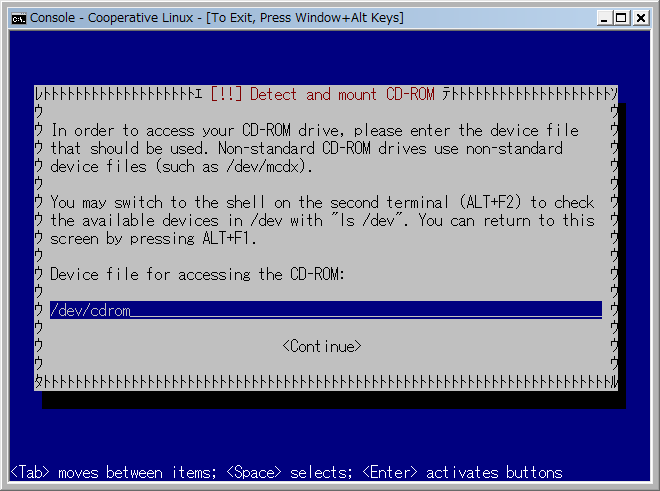
\includegraphics[width=100mm]{image200808/colinux_cdrom.png}
 \end{center}
 \caption{CD-ROMのマウント}
 \label{fig:colinux_cdrom}
\end{figure}

しかし、インストーラはcoLinuxが設定してくれたCD-ROMドライブにアクセスするためのデバイスファイルを
作成していないため、このままではCD-ROMにアクセスすることができません。

そこで、coLinuxが設定してくれた各種デバイスにアクセスするための、
デバイスファイルを作成します。

[ALT] + [F2] キーを押し、インストーラ画面からターミナルに移動します。
移動すると、図\ref{fig:colinux_secound_console}のような画面が表示されます。

\begin{figure}[htbp]
 \begin{center}
  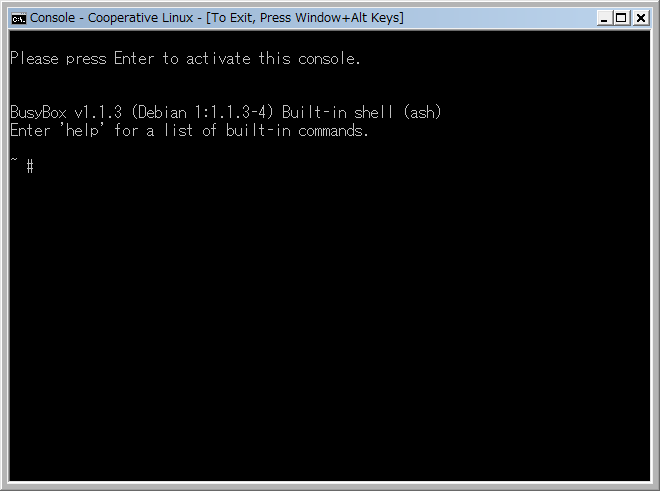
\includegraphics[width=100mm]{image200808/colinux_secound_console.png}
 \end{center}
 \caption{ターミナルに移動}
 \label{fig:colinux_secound_console}
\end{figure}

ターミナルにて以下のコマンドを入力します。

\begin{commandline}
# デバイスファイル/dev/cobdxを作成します。
i=0; while [ $i -lt 32 ]; do mknod /dev/cobd$i b 117 $i; i=`expr $i + 1`; done

# 環境によっては「mknod: /dev/cobdx: File exists」と言うメッセージが表示されることがありますが、
# これは既に/dev/cobdxが作成されているということですので、
# そのまま次に進めてもらっても問題ありません。

# デバイスファイル/dev/cofsxを作成します。
i=0; while [ $i -lt 16 ]; do mknod /dev/cofs$i b 117 $i; i=`expr $i + 1`; done
\end{commandline}

これでcoLinuxが設定してくれたCD-ROMをマウントすることができるようになりましたので、
[ALT] + [F1] キーを押し、ターミナルからインストーラ画面に戻ります。
戻ると、先程中断した図\ref{fig:colinux_cdrom}の画面が表示されますので、
以下の手順に沿ってインストール作業を進めていきます。

\begin{commandline}
# CD-ROMをマウントするため、DebianのISOイメージが設定されているデバイスファイルを指定します。
# 今回はdebian-install.confの7行目にて以下のように設定していますので、「/dev/cobd3」を指定します。
# cobd3="\DosDevices\C:\coLinux\debian-40r1-i386-businesscard.iso"
* 「/dev/cobd3」と入力し<Continue>

# カーネルモジュールはcoLinuxのものを使用しますので、読み込まずにインストールを続けます。
* <Yes>

# ネットワークを設定が行われますが、Windows側で設定が済んでいればDHCPで取得できますので、
# 特に何かする必要はありません。
\end{commandline}

ネットワークの設定が終わると、以降のインストールはDebianのインストールでは行えませんので、
続きの作業は手動にて行っていきます。

[ALT] + [F2] キーを押し、再びターミナルに移動し、
以下のコマンドを順次実行していきます。

\begin{commandline}
# まずはswapファイルを作成し、有効化します。
# 今回はdebian-install.confの4行目にて以下のように設定していますので、
# 「/dev/cobd0」に対してmkswapを実行します。
# cobd0="\DosDevices\C:\coLinux\swap_fs"
mkswap /dev/cobd0
sync; sync; sync
swapon /dev/cobd0

# 次に、coLinuxをインストールするために用意したディスクイメージに
# ext3ファイルシステムを作成します。
# 今回はdebian-install.confの5, 6行目にて以下のように設定していますので、
# 「/dev/cobd1」、「/dev/cobd2」に対してmke2fsを実行します。
# cobd1="\DosDevices\C:\coLinux\root_fs"
# cobd2="\DosDevices\C:\coLinux\home_fs"
mke2fs -j /dev/cobd1
mke2fs -j /dev/cobd2

# インストール対象の「/」をマウントするためのディレクトリを作成し、マウントします。
mkdir /target
mount /dev/cobd1 /target
cd /target

# coLinux附属のカーネルモジュールを使用するため、c:\coLinuxをマウントし、
# c:\coLinux\vmlinux-modules.tar.gzを\texttt{/target}に展開します。
mkdir -p /mnt/windows
mount -t cofs /dev/cofs0 /mnt/windows
tar -zxvf /mnt/windows/vmlinux-modules.tar.gz

# /targetにcoLinuxの設定するデバイスファイルを作成します。
mkdir /target/dev
i=0; while [ $i -lt 32 ]; do mknod /target/dev/cobd$i b 117 $i; i=$((i+1)); done
i=0; while [ $i -lt 16 ]; do mknod /target/dev/cofs$i b 117 $i; i=$((i+1)); done

# /targetにetcディレクトリを作成し、各種設定ファイルを作成しておきます。
mkdir /target/etc

# HTTPプロキシが必要な環境に接続されている場合、プロキシの設定を行います。
export http_proxy=http://myproxy.co.jp:8888

# debootstrapにて最小構成のDebianディレクトリツリーを作成します。
# ここではetchを指定していますが、sidやlennyを指定することもできます。
debootstrap --arch i386 etch /target http://cdn.debian.or.jp/debian/

# /targetにchrootし、インストール環境を設定していきます。
chroot /target

# /target/etc/fstabにインストール後のマウント情報を作成します。
cat <<EOF > /etc/fstab
/dev/cobd0 swap  swap defaults 0 0
/dev/cobd1 /     ext3 defaults 1 1
/dev/cobd2 /home ext3 defaults 1 1
proc       /proc proc defaults 0 0
EOF

# ネットワーク関連を設定します。
# お使いのcoLinuxの設定に合わせて行ってください。
cat <<EOF >> /etc/network/interfaces
auto lo
iface lo inet loopback
auto eth0
#iface eth0 inet dhcp
iface eth0 inet static
  address 192.168.0.10
  netmask 255.255.255.0
  gateway 192.168.0.1
EOF

echo "nameserver 192.168.0.1" > /etc/resolv.conf

echo "coLinux" > /etc/hostname

cat <<EOF >> /etc/hosts
127.0.0.1      localhost
192.168.0.10   coLinux
EOF

ln -sf /usr/share/zoneinfo/Japan  /etc/localtime

# shadowパスワードを有効にします
shadowconfig on

# aptリポジトリを設定します。
# ここではetchを指定していますが、sidやlennyを指定することもできます。
cat <<EOF > /etc/apt/sources.list
deb http://cdn.debian.or.jp/debian etch main contrib non-free
deb-src http://cdn.debian.or.jp/debian etch main contrib non-free
EOF

# ロケール関連を設定します。
aptitude update
aptitude -y install console-common
dpkg-reconfigure console-data

aptitude -y install locales
dpkg-reconfigure locales
\end{commandline}

これで基本となるインストール作業は完了したため、
Debianインストーラを終了させます。

[ALT] + [F1] キーを押し、ターミナルからインストーラ画面に移動し、
以下の手順に従ってインストーラを終了させます。

\begin{commandline}
# Debianインストーラを終了させます。
[ESC]キーを押下し、ネットワーク設定画面に戻ります。
もう一度[ESC]キーを押下し、メインメニューに戻ります。
メニュー一番下の「Abort the installation」を選択し[Enter]を押下します。
* <Yes>
\end{commandline}
これでcoLinuxが再起動されますが、設定ファイルがインストール起動用となっているため、
再びDebianインストーラが起動されますので、一旦coLinuxを終了させます。

\subsubsection{coLinuxを通常起動用に設定}
coLinuxへのDebianインストールは完了しましたので、
通常起動するためにcoLinuxの設定を変更します。

coLinuxインストールディレクトリにdebian.confと言う名前でファイルを作成し、
以下の内容を記載して保存します。

\begin{commandline}
kernel=vmlinux
initrd=initrd-normal.gz
mem=512
cobd0="\DosDevices\C:\coLinux\swap_fs"
cobd1="\DosDevices\C:\coLinux\root_fs"
cobd2="\DosDevices\C:\coLinux\home_fs"
eth0=tuntap
root=/dev/cobd1
ro
\end{commandline}

あとは、この設定ファイルを使用してcoLinuxを起動すると、
先程インストールしたオリジナルイメージで起動することができます。
コマンドプロンプトを起動し、\verb|c:\coLinux|にcdしてから、
以下のコマンドを実行します。

\begin{commandline}
colinux-daemon.exe -t nt "@c:\coLinux\debian.conf"
\end{commandline}



\subsection{XmingによるXアプリケーション起動方法}
coLinuxにはディスプレイデバイスが実装されていないため、
そのままではCUI環境でしか使用することができません。
しかし、XサーバやVNC、sshのX11フォワードなどの機能を使用すると、
Xアプリケーションを使用することができます。

今回はXmingを使用した、sshのX11フォワードとXDMCPについて紹介したいと思います。

sshのXフォワードでは必要ないのですが、XDMCP接続では、
ログインマネージャを使用する必要がありますので、
ログインマネージャとしてGDMを使用したXDMCP接続について説明したいと思います。

大まかな手順は以下のようになります。
\begin{enumerate}
\item Xmingのインストール
\item Xアプリケーションのインストール
\item sshのXフォワードで起動
\item XDMCPで起動
\end{enumerate}


\subsubsection{Xmingのインストール}
Xmingの配布サイト\footnote{\url{http://sourceforge.net/projects/xming/files}}から、
Xmingのインストーラ\footnote{執筆時ではXming-6-9-0-31-setup.exeが最新版となっています}と
コアXフォントのインストーラ\footnote{執筆時ではXming-fonts-7-3-0-22-setup.exeが
最新版となっています}をダウンロードし、インストールします。


\subsubsection{Xアプリケーションのインストール}
起動するXアプリケーションのインストールを行います。
ここではiceweaselをサンプルとして起動してみたいと思いますので、
iceweaselをインストールしておきます。

また、XDMCPで起動する方法もご紹介いたしますので、
XDMCP接続時のログインマネージャとしてGDMをインストールします。

\begin{commandline}
sudo aptitude install ssh gdm iceweasel
\end{commandline}

GDMをインストールすると、Debian起動時にGDMが起動しようとするのですが、
ディスプレイデバイスを持たないcoLinuxではGDM起動に失敗してしまい、
図\ref{fig:colinux_gdmerror}のようなエラー画面が表示されます。

\begin{figure}[htbp]
 \begin{center}
  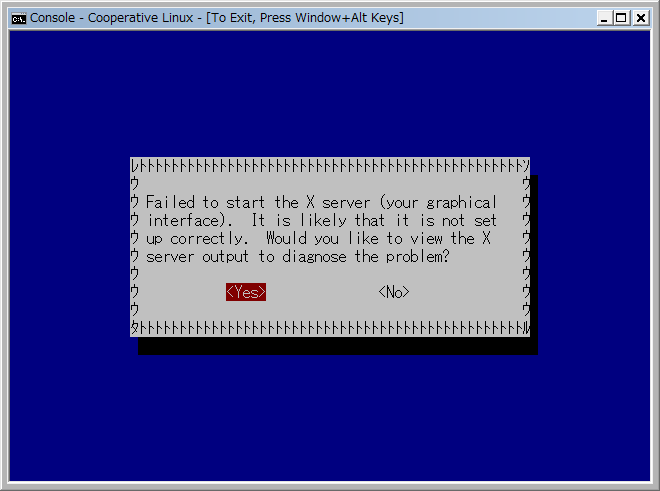
\includegraphics[width=100mm]{image200808/colinux_gdmerror.png}
 \end{center}
 \caption{ターミナルに移動}
 \label{fig:colinux_gdmerror}
\end{figure}

エラーが表示されても、問題なく使用できるですが余り気持ちの良いものではないため、
GDMのインストールが完了したらすぐに、GDMが起動しないように設定します。

\ref{/usr/share/gdm/defaults.conf}を以下のように書き換えます。
\begin{commandline}
   [servers]
-  0=Standard
+  #0=Standard
\end{commandline}

次に/etc/gdm/gdm.confを以下のように書き換えます。
\begin{commandline}
   [xdmcp]
+  Enable=true
\end{commandline}

設定がうまく行えたことを確認するため、
一旦Debianを再起動し、エラーが表示されないことを確認します。

\subsubsection{sshのXフォワードで起動する}
Xmingには、XLaunchというXmingを指定した設定で起動するためのツールが附属しています。
ここではXLaunchを使用して起動してみたいと思います。
まずXLaunchを起動すると、図\ref{fig:colinux_xlaunch}のようなDisplay setting画面が起動されます。
\begin{figure}[htbp]
 \begin{center}
  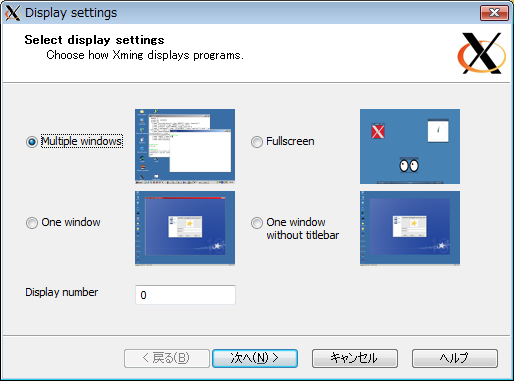
\includegraphics[width=100mm]{image200808/colinux_xlaunch.png}
 \end{center}
 \caption{XLaunch起動}
 \label{fig:colinux_xlaunch}
\end{figure}

起動方法が4種類あるのですが、表\ref{tab:display_setting}のような種類があります。
\begin{table}[htbp]
\begin{center}
  \begin{tabular}[htbp]{|l|l|}\hline
    モード & 表示方法\\ \hline\hline
    Multiple window & 起動するアプリケーション毎にwindowが起動します\\ \hline
    Fullscreen & X Window Systemがフルスクリーンで起動します。\\ \hline
    One window & 1つのwindowにX Window Systemが起動します\\ \hline
    One window whithout titlebar & One windowと同様ですが、タイトルバーが表示されません\\ \hline
  \end{tabular}
  \caption{ディスプレイ設定の選択}
  \label{tab:display_setting}
\end{center}
\end{table}

FullscreenやOne windowはXDMCPでも起動できますので、
ここではMultiple windowで起動してみます。

Multiple windowを選択して「次へ」を選択すると、
Session type画面が表示され、セッションタイプについて聞かれますので、
SSHを使用するStart a programを選択して「次へ」を選択します。
\begin{figure}[htbp]
 \begin{center}
  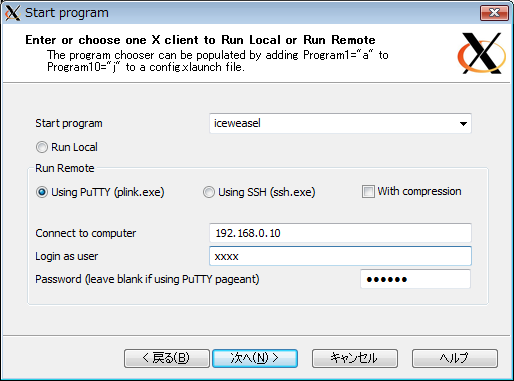
\includegraphics[width=100mm]{image200808/colinux_xlaunch_program.png}
 \end{center}
 \caption{XLaunch起動}
 \label{fig:colinux_xlaunch_program}
\end{figure}

すると図\ref{fig:colinux_xlaunch_program}のようなStart program画面が表示されますので、
Start programに起動するXアプリケーションを指定します。
ここではiceweaselを起動するため、iceweaselと入力します。
Using PuTTY(plink.exe)を選択し、Connect to computerにcoLinuxのIPを入力します。
coLinuxの名前解決ができるようであればホスト名を入力しても問題ありません。
Login as userにユーザ名を入力し、パスワードを入力し、「次へ」を選択します。

Additional parameters画面が表示されますが、
特に指定する必要はありませんので、そのまま「次へ」を選択します。

Finish configuration画面が表示されますので、
「完了」を選択すると、iceweaselが起動します。
「Save configuration」を選択すると、今回行った設定を保存することができます。
Include PuTTY Password as insecure clear textにチェックを入れると、
設定ファイルにパスワードを保存することができますが、
平文で保存されますので注意が必要となります。

保存された設定ファイルをダブルクリックすると、
Xmingが起動され、sshで接続を行い、iceweaselを簡単に起動することができるようになります。

\subsubsection{XDMCPで起動する}
XDMCPの起動では、表\ref{tab:display_setting}のモードの内、
Multiple window以外の起動方法で表示することができます。
ここではOne windowで起動してみます。

XLaunchを起動し、Display setting画面にてOne windowを選択して「次へ」を選択すると、
Session type画面が表示され、セッションタイプについて聞かれますので、
Open session via XDMCPを選択して「次へ」を選択します。
\begin{figure}[htbp]
 \begin{center}
  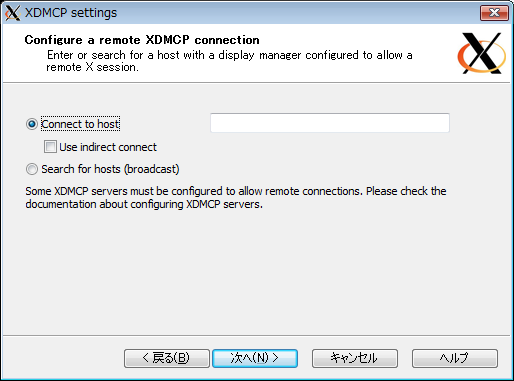
\includegraphics[width=100mm]{image200808/colinux_xlaunch_xdmcp.png}
 \end{center}
 \caption{XLaunch起動}
 \label{fig:colinux_xlaunch_xdmcp}
\end{figure}

すると図\ref{fig:colinux_xlaunch_xdmcp}のようなXDMCP setting画面が表示されますので、
Connect to hostにcoLinuxのIPアドレスを入力します。
coLinuxの名前解決ができるようであればホスト名を入力しても問題ありません。
Additional parameters画面が表示されますが、
特に指定する必要はありませんので、そのまま「次へ」を選択します。

Finish configuration画面が表示されますので、
「完了」を選択すると、GDMが起動し、ログイン画面が表示されます。

「Save configuration」を選択すると、今回行った設定を保存することができます。
ログインが完了すると、GNOME環境が起動しますので、
Application→Internet→Iceweasel Web Browserを選択し、iceweaselを起動します。

以上駆け足でしたが、coLinuxにDebianを新規インストールしたり、
ディスプレイデバイスを持たないcoLinuxでのXアプリケーションの起動について紹介いたしました。

% kansairesume200809

%% takaya
\dancersection{Debian Live に Ubiquity を移植できるか?}{山下 尊也}
\label{sec:ubiquity}

% \subsection{Ubiquityって何してるの?}

% Ubiquity is a simple graphical live CD installer designed to integrate
% well with Debian- and Ubuntu-based systems、 written largely in Python、
% using d-i as a backend for many of its functions for ease of
% maintenance。

% Ubiquityは大部分がPythonで書かれており、
% メンテナンスの簡潔さのためにそのほとんどの関数を Debian Installer を使用
% しております。Debian と Ubuntu ベースのシステムでLive CDに統合したデザイ
% ンのインストーラです。

\subsection{Ubiquityパッケージをビルドする}

\url{http://jp.archive.ubuntu.com/ubuntu/}からubiquityのソースを取って
きます。

今回、私は、
{\tt ubiquity\_1.8.12.tar.gz}
をダウンロードしてきました。

なんとか、snapshot.debianやソースパッケージを用いて、依存関係を解決しま
した。\footnote{rulesの変更だけしたら大丈夫かも?本来はちゃんとした依存
関係を調べないといけません。}

しかし、ビルドの行程で、
{\tt /usr/share/iso-codes/iso\_3166.tab}
が存在しないと怒られます。
{\tt iso\_3166.tab}
は、地理情報を表しているものです。
調べてみたところ、sargeやetchにはiso-3166-udebと言う形で提供されています
が、lennyからは、iso-3166-udebパッケージが廃止されています。

調べていく過程で、tzdataパッケージに、
iso3166.tabと言うファイルが存在する事が分かりました。
中身を見たところ、これを利用すればDebianでもビルド出来そうです。
今回は、時間がなかったため、
{\tt iso\_3166.tab}
をUbuntu Hardyが起動している環境から持ってきて、利用しました。

なんとか、以下のパッケージを作成する事が出来ました。
\begin{itemize}
 \item {\tt ubiquity-frontend-gtk\_1.8.12\_i386.deb}
 \item {\tt ubiquity-frontend-kde\_1.8.12\_all.deb}
 \item {\tt ubiquity-frontend-mythbuntu\_1.8.12\_all.deb}
 \item {\tt ubiquity-ubuntu-artwork\_1.8.12\_all.deb}
 \item {\tt ubiquity\_1.8.12\_i386.deb}
\end{itemize}

また、
{\tt d-i/source/localechooser/mkshort}
を変更し、
{\tt /usr/share/zoneinfo/iso3166.tab}
を用いる変更を加えれば、
この問題は解決出来そうです。

\subsection{Ubiquity で必要になるパッケージ}

\subsubsection{Ubiquity 関係パッケージの Depends で関係するもの}
\label{sec:depends}

Ubuntu Hardyが起動している環境から、
{\tt /var/lib/apt/lists/}
ディレクトリ下にある

{\tt jp.archive.ubuntu.com\_ubuntu\_dists\_hardy\_main\_binary-i386\_Packages}

を持ってきて、ubiquity関連パッケージのDependsに書かれている
ものを書き出したものが以下のものです。

\begin{commandline}
adduser
console-setup
debconf
grub
iso-codes
kwin
laptop-detect
libatk1.0-0
libc6
libcairo2
libdebconfclient0
libdebian-installer4
libffi4
libglib2.0-0
libgtk2.0-0
libpango1.0-0
libparted1.7-1
libxml2
lsb-release
os-prober
passwd
python
python-apt
python-central
python-glade2
python-gtk2
python-qt4
sudo
ubiquity
ubiquity-artwork-1.8.7
ubiquity-casper
ubiquity-frontend-1.8.7
x-window-manager
\end{commandline}

同様に、Debian Lennyが動いている環境の{\tt /var/lib/apt/lists/}にある

\begin{itemize}
 \item {\tt cdn.debian.or.jp\_debian\_dists\_lenny\_main\_binary-i386\_Packages}
 \item {\tt cdn.debian.or.jp\_debian\_dists\_lenny\_contrib\_binary-i386\_Packages}
 \item {\tt cdn.debian.or.jp\_debian\_dists\_lenny\_non-free\_binary-i386\_Packages}
\end{itemize}

をチェックしたところ、Debian Lennyには以下のパッケージが存在しない事が
分かりました。

\begin{commandline}
libffi4
libparted1.7-1
ubiquity
ubiquity-artwork-1.8.7
ubiquity-casper
ubiquity-frontend-1.8.7
x-window-manager
\end{commandline}

libffi4は、etchに存在し、
libparted1.7-1は、ソースからビルドすれば、パッケージの作成をする事が出来
ます。\footnote{現在、automake1.8とのバグのため、ビルド出来ない状況になっ
ているため、今回は、snapshot.debianからパッケージをダウンロードしました。}

x-window-managerは仮想パッケージのため、このリストには存在しません。
と言うことで、依存関係は解決出来たみたいです。

\subsection{Debian Liveに依存関係を解決し、入れてみる}

OSC Kansaiで配布したDebian Liveで使われていたものをある程度、
利用したいため、git hubから取ってきて、\ref{sec:depends}で追加したリストを追記します。

\begin{commandline}
 % git clone git://github.com/nogajun/debian-study-live-cd.git
 % vi debian-study-live-cd/config/chroot_local-packageslists/06-ubiquity
\end{commandline}

また、GTKの環境だけを考えているため、以下のパッケージをインストールする事を考
えます。

\begin{commandline}
ubiquity-frontend-gtk_1.8.12_i386.deb
ubiquity-ubuntu-artwork_1.8.12_all.deb
ubiquity_1.8.12_i386.deb 
\end{commandline}

% \verb|debian-study-live-cd/config/chroot_local-packages|
{\tt debian-study-live-cd/config/chroot\_local-packages|}
ディレクトリに入れ、パッケージの正当性チェックを無効にしておきます。

\begin{commandline}
 % sudo lh_build
\end{commandline}

しかし、ここでまたもや、依存関係のエラーがでます。

\begin{commandline}
  libffi4: Depends: gcc-4.1-base (= 4.1.1-21) but it is not going to be installed
  ubiquity: Depends: ubiquity-casper but it is not installable 
\end{commandline}

とりあえず、リストの前に追加しますが、ubiquity-casperは、Ubuntuにしかあ
りません。
ubiquity-casperは、live installerからの設定を行うものですが、
これをソースからビルドすると

\begin{commandline}
Some packages could not be installed. This may mean that you have
requested an impossible situation or if you are using the unstable
distribution that some required packages have not yet been created
or been moved out of Incoming.
The following information may help to resolve the situation:
 casper: Depends: busybox-initramfs (>= 1:1.1.3-4ubuntu3) but it is not installable
         Depends: localechooser-data but it is not installable
 libffi4: Depends: gcc-4.1-base (= 4.1.1-21) but it is not going to be installed
E: Broken packages
\end{commandline}

Ubiquityの問題ではなく、依存関係をどうするかを考えた方が良かったみたいで
す。少しずつ時間を見つけて、依存関係を見直していこうと思います。


\dancersection{10分でわかる Debianフリーソフトウェアガイドライン (DFSG)}{木下 達也}
\subsection{Debianフリーソフトウェアガイドラインとは}

ある著作物が「フリー」かどうか、
フリー(自由な)OSであるDebianの構成要素として
適しているかどうかを判定する際の基準、それが
Debianフリーソフトウェアガイドライン
(DFSG: Debian Free Software Guidelines)です。

\url{http://www.debian.org/social_contract#guidelines}
 
フリー(自由な)ソフトウェアとは、自由に使ったり、
変更したり、コピーして配ったりできるソフトウェアの
ことをいいます。

ただし、「自由」とはいっても、無制限というわけではなく、
ある種の制約は認められています。
(著作権表示・ライセンスの維持、変更の明示など)

\subsection{著作権とライセンス}

著作物には、基本的に著作者に対して「著作権」
が発生しています。

つまり、著作物を変更したりコピーして配ったりするには、
著作者からの許可(ライセンス)が必要になります。

ライセンスは次のように確認します。

\begin{itemize}
 \item 変更や配布が許可されているか
 \item それらに付随する制約はどうか
\end{itemize}

その他、個別の事情も検討する必要があります。
(特許、商標など)

\newpage
\subsection{Debianフリーソフトウェアガイドラインの説明}

\begin{itemize}
 \item 1. 自由な再配布 (Free Redistribution)

有償・無償を問わず、
別途の許可を必要とすることなく、
プログラムを複数まとめて配布できる。

(Artistic License: プログラム単体への課金は禁止、複数まとめての販売は可)

 \item 2. ソースコード (Source Code)

ソースコード(変更に適した形式)が必要。

実行形式だけでなくソースコードでも配布できる。

 \item 3. 派生ソフトウェア (Derived Works)

同様のライセンスで変更版を配布できる。

(GNU GPL: 変更版全体に同様のライセンスを強制)

(BSD License: 変更版全体には別ライセンスの適用可)

 \item 4. 原作者によるソースコードの整合性維持
   (Integrity of The Author's Source Code)

変更版のソースコードを配布する場合に、
元のソースコードと差分(パッチ)という形式のみ許可
という制約は許容、ただし非推奨。

(QPL: 元のソースコードと差分の要求)

 \item 5. すべての個人、団体の平等
   (No Discrimination Against Persons or Groups)

いかなる個人・団体も差別せずに許可。

 \item 6. 目標分野の平等
   (No Discrimination Against Fields of Endeavor)

商用・非商用・平和利用・軍事目的など、用途を制限しない。

 \item 7. ライセンスの配布
   (Distribution of License)

ライセンスは、再配布されたすべての人々に、
別途の許可を必要とすることなく、適用される。

 \item 8. ライセンスはDebianに限定されない
   (License Must Not Be Specific to Debian)

Debianの一部としてのみの許可ではなく、
他のシステムにも適用できるように。
特定の製品に依存しないように。

 \item 9. ライセンスは他のソフトウエアを侵害しない
   (License Must Not Contaminate Other Software)

たとえば、同じ媒体で配布されるソフトウエアすべてが
フリーソフトウエアであることを要求しないように。

 \item 10. フリーなライセンスの例
   (Example Licenses)

GNU GPL, BSD License, Artistic License

(私見としては、Artistic Licenseは推奨しません。
Free Software Foundationでは「曖昧過ぎる」としてNon-Freeに分類されています)

\url{http://www.gnu.org/licenses/license-list.ja.html#ArtisticLicense}

\end{itemize}

% kansairesume200810
\dancersection{はじめての CDBS}{佐々木 洋平}
\index{cdbs}

\subsection{はじめに}

CDBS -- {\bf C}ommon {\bf D}ebian {\bf B}uild {\bf S}ystem は、
\texttt{debian/rules} の共通部分を抽出し共有することで、 
\texttt{debian/rules} を簡潔かつ理解しやすくすることを目的としたツールです。
%
\cite{lenny CDBS doc} の Introduction によれば、 当初の開発動機は GNU
autoconf \& GNU automake を使用している Debian パッケージの重複した
\texttt{debian/rules} をなんとかしたい、 だった様です:
\begin{quotation}
    The motivating factor for CDBS was originally that more and more
    programs today are created using GNU Autoconf configure scripts and
    GNU Automake, and as such they are all very similar to configure and
    build.  It was realized that a lot of duplicated code in everyone's
    debian/rules could be factored out. ...
\end{quotation}

今では CDBS はもっと汎用的になっており、 
autotools に限らず、 Gnome、 KDE、 Python、 Haskell など、 
様々なパッケージの作成に使用できるようになっています。
%
\cite{CDBS ギャラリ岩松版}によると、
現時点で CDBS を使用しているソースパッケージは 3145 個、
ソースパッケージ全体の $\sim 23 \%$ だそうです。

ドキュメントで挙げられている CDBS の利点は以下の通りです%
\footnote{%
\cite{CDBS doc} の CDBS advantages の超訳です - -;)
}:
\begin{enumerate}
    \item 簡潔で、可読性が高く、効率的な \texttt{debian/rules} を作成できる。
    \item debhelper と autotools の呼び出しを自動化することによって、
          繰り返し作業を気にする必要がなくなる。\index{debhelper}
    \item カスタマイズ性に限界が無いので、
          メンテナはパッケージ作成時のより重要な問題に集中できる。
    \item 提供されるクラスは十分にテストされており、
          よくある問題を回避するための汚い hack をする必要がない。
    \item 既存のパッケージを CDBS へ移行するのは容易である。
    \item 拡張性が高い。
\end{enumerate}
確かにそうなんですけれども、 
以下の例では逆に何をしているのかわからなくて不安になったりします:
\begin{commandline}
#!/usr/bin/make -f
                                
include /usr/share/cdbs/1/rules/debhelper.mk
include /usr/share/cdbs/1/class/autotools.mk
\end{commandline}

ここでは \cite{CDBS doc} の冒頭をざっくり解説してみようと思います。

\subsection{CDBS のディレクトリ構成\& ファイル群}

CDBS の実態は細分化された Makefile 群です。
実際に \url{/usr/share/cdbs/} 以下を眺めてみましょう:
\begin{commandline}
% ls -aR /usr/share/cdbs
/usr/share/cdbs/:
./  ../  1/

/usr/share/cdbs/1:
./  ../  class/  rules/

/usr/share/cdbs/1/class:
./                  autotools-vars.mk  hbuild.mk         perlmodule-vars.mk
../                 autotools.mk       kde.mk            perlmodule.mk
ant-vars.mk         cmake.mk           langcore.mk       python-distutils.mk
ant.mk              docbookxml.mk      makefile-vars.mk  qmake.mk
autotools-files.mk  gnome.mk           makefile.mk

/usr/share/cdbs/1/rules:
./   buildcore.mk  debhelper.mk  patchsys-quilt.mk   tarball.mk
../  buildvars.mk  dpatch.mk     simple-patchsys.mk  utils.mk
\end{commandline}
中間ディレクトリ{\bf 1} は
将来の API 変更を考慮したディレクトリです。
rules、 class ディレクトリ以下にあるファイルが
細分化された Makefile です。
パッケージを作成する際には
これらのファイルを適宜 \texttt{debian/rules} 内で include して使用します。
個々の Makefile の依存関係は\fgref{fig:cdbs-mk-depend}の通りです:
%
\begin{figure}[htbp!]
 \begin{center}
  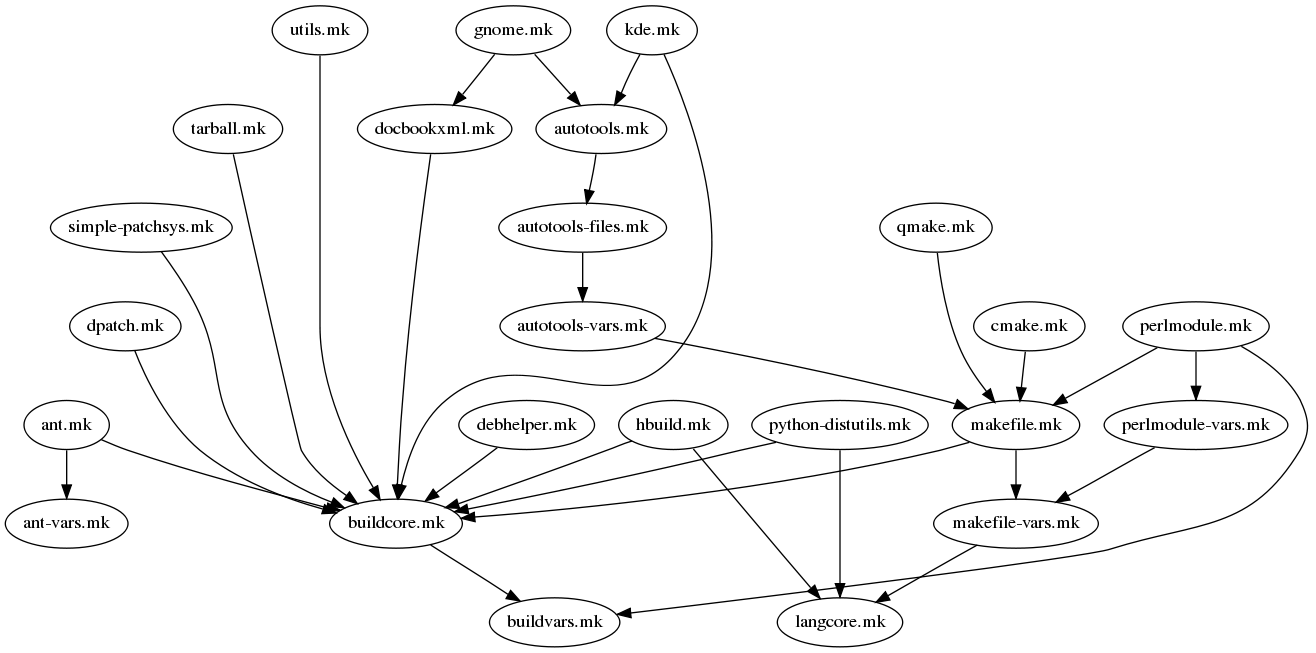
\includegraphics[width=160mm]{image200810/cdbs-mk-depend.png}
 \end{center}
    \caption{%
    CDBS で提供される Makefile の依存関係
    (\cite{lenny CDBS doc}).
    }
    \label{fig:cdbs-mk-depend}
\end{figure}

\subsection{基本となる rules}
\label{section:rules}

\subsubsection{buildvars.mk}

buildvars.mk を include すると
パッケージ作成のための環境変数が設定されます。
%
設定される変数の一覧を表 \ref{table:buildvars.mk} に記載します。
%
良く使われるのは {\tt CURDIR} と {\tt DEB\_DESTDIR} でしょう。
%
\begin{table}[htbp!]
    \begin{center}
     \caption{\url{/usr/share/cdbs/1/rules/buildvars.mk} で設定される変数}
        \label{table:buildvars.mk}
        {\small 
        \begin{tabular}[tb]{|l|l|}
            \hline
            {\tt CURIDR} & 
            パッケージを作成しているディレクトリの名前。\\
            \hline
            {\tt DEB\_SOURCE\_PACKAGE} & 
                ソースパッケージの名前。\\
            \hline
            {\tt DEB\_VERSION} & 
                完全な Debian Version。\\
            \hline
            {\tt DEB\_NOEPOCH\_VERSION} & 
                Debian version without epoch 。\\
            \hline
            {\tt DEB\_ISNATIVE} & 
                native パッケージの場合は空ではない(条件分岐に使用)。\\
            \hline
            {\tt DEB\_ALL\_PACKAGES} & 
                作成される全てのパッケージのリスト。\\
            \hline
            {\tt DEB\_INDEP\_PACKAGES} & 
                アーキテクチャに依存しないパッケージのリスト。\\
            \hline
            {\tt DEB\_ARCH\_PACKAGES} & 
                アーキテクチャに依存するパッケージのリスト。\\
            \hline
            {\tt DEB\_PACKAGES} & 
                通常の(udeb ではない)パッケージのリスト。\\
            \hline
            {\tt DEB\_UDEB\_PACKAGES} & 
                udeb の場合、 そのリスト。\\
            \hline
            {\tt DEB\_ARCH} & 
                Debian アーキテクチャ。 後方互換のために残されている。\\
            \hline
            {\tt DEB\_HOST\_ARCH\_CPU} & 
                Debian アーキテクチャの CPU 情報。\\
            \hline
            {\tt DEB\_HOST\_ARCH\_OS} & 
                Debian アーキテクチャの OS 情報。\\
            \hline
            {\tt DEB\_DESTDIR} & 
                パッケージ作成の際にソフトを install するディレクトリ。\\
            & 単一パッケージの場合は {\tt \$(CURDIR)debian/パッケージ名} \\
            & 複数のパッケージを作成する場合には {\tt \$(CURDIR)debian/tmp}\\
            \hline
        \end{tabular}
        }
    \end{center}
\end{table}
これらの変数を変更したい場合には、 buildvars.mk を include した後で
\texttt{debian/rules} 内部で以下の様に設定します:
\begin{commandline}
# where sources are
DEB_SRCDIR = $(CURDIR)/src
# in which directory to build
DEB_BUILDDIR = $(DEB_SRCDIR)/build
# in which directory to install the sofware
DEB_DESTDIR = $(CURDIR)/destination
\end{commandline}

\subsubsection{buildcore.mk によるターゲットの設定}

buildcore.mk はパッケージ作成のための基本的なターゲットを提供します。
\cite{ポリシー}によれば、 パッケージ作成の際
\texttt{debian/rules} ファイルの中で外部から参照されうるターゲットは、
以下の通りです:
\begin{itemize}
    \item build
    \item binary, binary-arch, binary-indep
    \item clean
    \item build-arch, build-indep (optional)
    \item get-orig-source (optional)
    \item path (optional)
\end{itemize}
buidcore.mk を include すると 
これらのターゲットが {\bf 細分化されて}提供されます。
buildcore.mk が提供する
ターゲットの一覧を図\ref{fig:cdbs-target}に示します。
%
\begin{figure}[htbp!]
 \begin{center}
  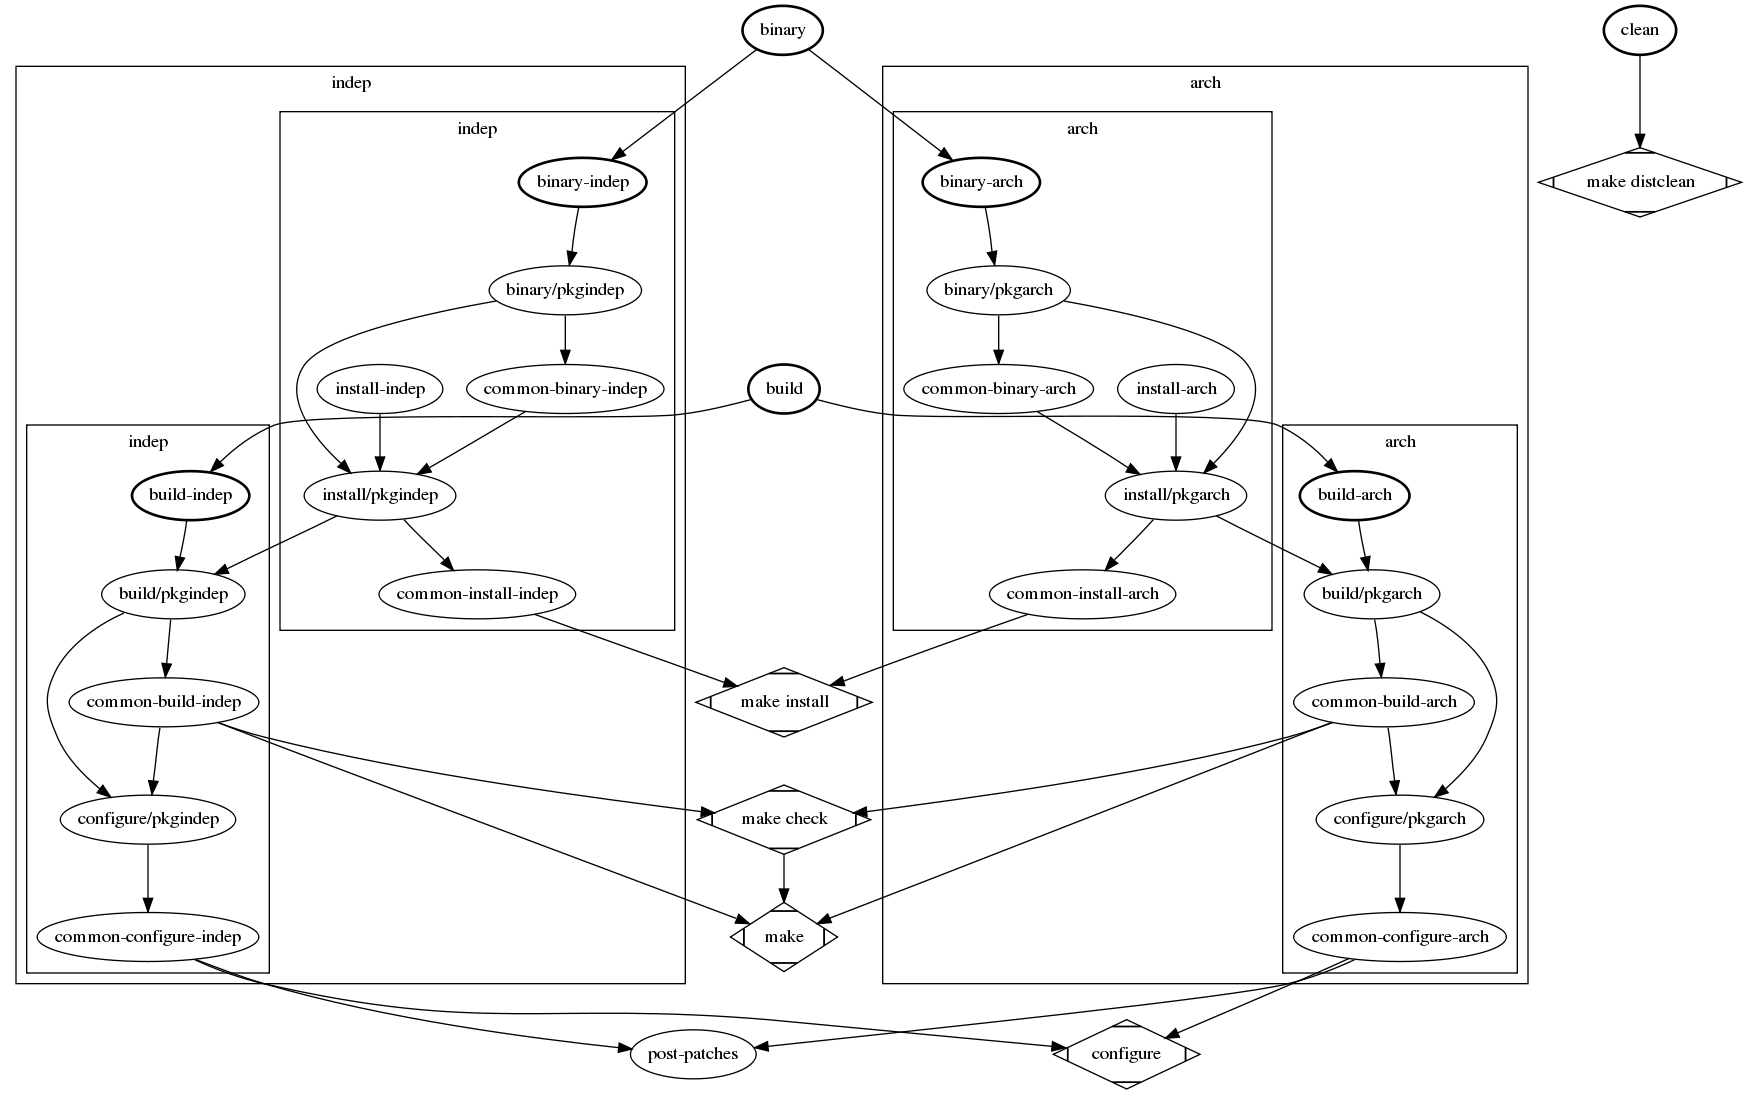
\includegraphics[width=160mm]{image200810/cdbs-target.png}
 \end{center}
    \caption{%
    buildcore.mk で提供されるターゲットの流れ
    (\cite{lenny CDBS doc})。
    }
    \label{fig:cdbs-target}
\end{figure}

実際には、 buildcore.mk 自体はパッケージに対してなんの処理もしません。 
よって適宜 rules を記述することになります。 
例として、 \cite{CDBS doc} に記載されている foo について解説します。
ここで foo は
\begin{itemize}
    \item ソースパッケージ foo を生成
    \item バイナリとして foo(arch-dep) と foo-data(arch-indep) を生成
\end{itemize}
するパッケージだとします。
\begin{commandline}
#!/usr/bin/make -f
include /usr/share/cdbs/1/rules/buildcore.mk

# pre-configure action
makebuilddir/foo::
        ln -s plop plop2
# post-configure action
configure/foo::
    sed -ri 's/PLOP/PLIP/' Makefile
configure/foo-data::
    touch src/z.xml
# post-build action
build/foo::
    /bin/bash debian/scripts/toto.sh
build/foo-data::
    $(MAKE) helpfiles
# post-install action
install/foo:
    cp debian/tmp/myfoocmd debian/foo/foocmd
      find debian/foo/ -name ``CVS'' -depth -exec rm -rf {} \;
install/foo-data:
    cp data/*.png debian/foo-data/usr/share/foo-data/images/
    dh_stuff -m ipot -f plop.bz3 debian/foo-data/libexec/
# post deb action
binary/foo:
    strip --remove-section=.comment --remove-section=.note --strip-unneeded \
      debian/foo/usr/lib/foo/totoz.so
# pre-clean action
cleanbuilddir/foo::
    rm -f debian/fooman.1
\end{commandline}
コメントとしてターゲットを記述するタイミングを記載しました。
ターゲットの記法は
\begin{center}
    {\tt {\bf target/packagename::}}
\end{center}
です。 後ろの {\tt {\bf ::}} が重要です。

\subsubsection{debhelper.mk による dh\_ の自動化}

CDBS の一番の御利益が、 この debhelper.mk です。
CDBS では主な dh\_\* コマンドの呼び出しを debhelper.mk において行なうため、
\texttt{debian/rules} 内の dh\_\* の殆んどが不要になります。
debhelper.mk によって呼び出される dh\_\* を
表\ref{table:debhelper.mk}に示します。
\begin{table}[htbp!]
    \begin{center}
        \caption{%
        \url{/usr/share/cdbs/1/rules/debhelper.mk} で管理される dh\_ コマンド}
        \label{table:debhelper.mk}
        \begin{tabular}[tb]{|llll|}
            \hline
            dh\_builddeb  & 
            dh\_installchangelogs  &
            dh\_installemacsen  & 
            dh\_installman   \\
            dh\_perl & 
                dh\_clean  & dh\_installcron  & dh\_installexamples \\
            dh\_installmenu  & 
                dh\_shlibdeps & dh\_compress  & dh\_installdeb  \\
            dh\_installinfo  & 
                dh\_installpam  & dh\_strip   & dh\_fixperms  \\
            dh\_installdebconf  & 
                dh\_installinit  & dh\_link  & dh\_gencontrol  \\
            dh\_installdirs  & 
                dh\_installlogcheck  & dh\_makeshlibs  & dh\_install  \\
             dh\_installdocs  & dh\_installlogrotate  & dh\_md5sums & \\
            \hline
        \end{tabular}
    \end{center}
\end{table}

debhelper.mk によって呼び出される dh\_ コマンドに対しては、
パラメータ設定は(大抵の場合)不要です。 
debelpher の呼び出しをカスタマイズする変数は 
debhelper.mk 冒頭のコメント行を参照して下さい。
\cite{CDBS doc} には以下の例があります:

\noindent {\bf 依存関係がシビアな共有ライブラリについて}
\begin{commandline}
DEB_DH_MAKESHLIBS_ARGS_libfoo := -V''libfoo (>= 0.1.2-3)``
DEB_SHLIBDEPS_LIBRARY_arkrpg := libfoo
DEB_SHLIBDEPS_INCLUDE_arkrpg := debian/libfoo/usr/lib/
\end{commandline}
\noindent {\bf ChangeLog のファイル名が一般的でない場合}
\begin{commandline}
DEB_INSTALL_CHANGELOGS_ALL := ProjectChanges.txt
\end{commandline}
\noindent {\bf .py を圧縮せずにパッケージ化する場合}
\begin{commandline}
DEB_COMPRESS_EXCLUDE := .py
\end{commandline}

ここでの記法
\begin{center}
    {\tt {\bf :=}}
\end{center}
に注意して下さい。
{\tt {\bf :=}} は上書きです。
CDBS の提供する変数に追加する場合には {\tt {\bf +=}} を使用します。

\subsubsection{patch の管理}

dpatch、 quilt、 そして CDBS 用の simple-patchsys の rules が提供されていま
す。  quilt、 dpatch については include するだけで patch を適用する rule が
適用されます。
%

simple-patchsys の場合は debian/patches に patch を置くだけ
で、 パッケージ作成時に patch を適用し clean の際には元に戻します。
patch level は 3 まで ok です。 自動的に適用しようと試みます。

\subsection{class を使用する}

前節で rules について簡単にまとめました。  
ここでは幾つかの class について紹介します。

\subsubsection{Makefile の場合:makefile.mk}

autotools を使わず Makefile のみを使用するソフトウェアには
makefile.mk が便利です。 
\cite{CDBS doc} では、
元々の Makefile が
\begin{itemize}
    \item 名前が MaKeFile で
    \item make mrproper で clean 
    \item make myprog で build
    \item make check  で check
    \item make install で install
\end{itemize}
というソフトウェアの場合について例示しています:
\begin{commandline}
#!/usr/bin/make -f
include /usr/share/cdbs/1/rules/debheper.mk
include /usr/share/cdbs/1/class/makefile.mk

DEB_MAKE_CLEAN_TARGET    := mrproper
DEB_MAKE_BUILD_TARGET    := myprog 
DEB_MAKE_INSTALL_TARGET  := install DESTDIR=$(CURDIR)/debian/tmp/
# no check for this software
DEB_MAKE_CHECK_TARGET    := check
# allow changing the makefile filename in case of emergency exotic practices
DEB_MAKE_MAKEFILE        := MaKeFiLe
# example when changing environnement variables is necessary :
DEB_MAKE_ENVVARS         := CFLAGS=''-fomit-frame-pointer''
\end{commandline}

\subsubsection{Autotoolsの場合: autotools.mk}

いわゆる {\tt configure \&\& make \&\& make install} なソフトウェアの場合は
autotools.mk が便利です。
%
冒頭にも例示しましたが、 
標準的な autotools を使用するソフトウェアの場合には
\begin{commandline}
#!/usr/bin/make -f

include /usr/share/cdbs/1/rules/debheper.mk
include /usr/share/cdbs/1/class/autotools.mk
\end{commandline}
となります。 

configure へのオプションや環境変数の設定を行なう場合には
以下の様にします:
\begin{commandline}
DEB_CONFIGURE_EXTRA_FLAGS := --with-ipv6 --with-foo
COMMON_CONFIGURE_FLAGS := --program-dir=/usr
DEB_CONFIGURE_SCRIPT_ENV += LDFLAGS='' -Wl,-z,defs -Wl,-O1''
\end{commandline}
ここでも {\tt +=}、 {\tt :=} の意味は変わりません。
例えば
\begin{commandline}
#!/usr/bin/make -f

include /usr/share/cdbs/1/rules/debheper.mk
include /usr/share/cdbs/1/class/autotools.mk

# normally
DEB_MAKE_INSTALL_TARGET := install DESTDIR=$(DEB_DESTDIR)
# example to work around dirty makefile
# DEB_MAKE_INSTALL_TARGET := install prefix=$(CURDIR)/debian/tmp/usr
DEB_MAKE_CLEAN_TARGET := distclean
# example to activate check rule
DEB_MAKE_CHECK_TARGET := check
# overriding make-only environnement variables :
# (should never be necessary in a clean build system)
# (example borrowed from the bioapi package)
DEB_MAKE_ENVVARS    := ``SKIPCONFIG=true''
\end{commandline}
など。

他にも Perl、 Python、 Ruby、 GNOME、 KDE、 Ant、 HBuild(Haskell) 用の 
class があります。

\subsection{まとまってないまとめ}

そんな所で締切の時間が来てしまいました。

CDBS を使いはじめたら、 もう debhelper には戻れない体になってしまうわけで
すが、 いかんせん CDBS ってドキュメント少ないんですよね。 
%
この文書が最初の一歩になれば幸いです。

\newpage
\begin{thebibliography}{99}
    \bibitem[CDBS Documentation Rev. 0.4.0]{CDBS doc}
                    Marc (Duck) Dequ\'enes,
                    Arnaud (Rtp) Patard, 
                    2007:
                    CDBS Documentation,
                    \url{http://perso.duckcorp.org/duck/cdbs-doc/cdbs-doc.xhtml}
                    \newline
                    CDBS の online ドキュメンテーションです。
                    パッケージに含まれているドキュメントより、 
                    こっちの方が情報が多く、 参考になります。
                    
    \bibitem[CDBS Documentation Rev.0.1.2]{lenny CDBS doc}
                    Marc (Duck) Dequ\'enes,
                    Arnaud (Rtp) Patard, 
                    Peter Eisentraut,
                    Colin Walters,
                    2007:
                    \url{/usr/share/doc/cdbs/cdbs-doc.html}.
                    \newline
                    Lenny の CDBS(ver. 0.4.52) 付属のドキュメントです。
                    Web で公開されているドキュメントよりは古いです。

    \bibitem[CDBS 移行への 1st step]{CDBS 1st}
                    Tatsuki Sugiura, 2006:
                    CDBS 移行への 1st step
                    \url{http://sugi.nemui.org/doc/cdbs/cdbs-trans-1st.html}\\
                    既存のパッケージを CDBS へ移行する場合、 
                    非常に参考になると思います。

    \bibitem[Online CDBS Gallery]{CDBS ギャラリ岩松版}
                    本家: Online CDBS Gallery,
                    \url{http://cdbs.ueberalles.net/index.html}\\
                    CDBS を使っている \texttt{debian/rules} を見ることが
                    できます。
                     新たに CDBS へ移行する際に参考になるでしょう。  ちなみ
                     に、 本家は 2006 年で更新が止まっている模様。 岩松さん
                     が nigauri.org に CDBS ギャラリを上げて更新して下さい
                     ました。
                 \url{http://www.nigauri.org/~iwamatsu/cdbs/archive/site/}
                    
    \bibitem[Debian Policy Manual]{ポリシー}
                    Ian Jackson \& Christian Schwarz, 1996:
                    Debian Policy Manual,
                    \url{http://www.debian.org/doc/debian-policy/}

    \bibitem[Debian パッケージ作成の手引き]{パッケージ手引き}
                    小林 儀匡, 
                    Debianパッケージ作成の手引き,
                    \url{http://www.debian.or.jp/~nori/debian-packaging-guide/index.html}
                    \newline
                    Debian パッケージ作成の手引きです。
                    「debhelper を使わない場合 → 
                    使う場合 →
                    CDBS への移行」と順序立てて説明されています。

    \bibitem[やまだ \& 鵜飼(2006)]{入門 Debian パッケージ}
                    やまだあきら(著), 鵜飼文敏(監修), 2006:
                    入門 Debian パッケージ, 技術評論社,
                    ISBN4-7741-2768-X \\
                    apt の使い方やDebian パッケージの作り方などを
                    順を追って解説しています。

\end{thebibliography}

%% araki
\dancersection{cdn.debian.or.jp, cdn.debian.netにおける取り組み}{荒木 靖宏}
\index{cdn.debian.net}
\index{cdn.debian.or.jp}

いつでも必要なソフトウェアやコンテンツを安価に入手する手段としてCDNが広
くつかわれている。 Debianはdebの安定入手手段の有無がシステム の信頼性を
左右するシステムであり、その特殊性を考慮したCDNシステムが必要となる。 今
回はcdn.debian.or.jp, cdn.debian.netにおける取り組みを紹介する。

\subsection{CDNとは}

Content Delivery Network(CDN)
\index{Content Delivery Network}はウェブコンテンツ配置および配送方法とし
てAkamai社によりサービスされ広く知られることになった。当初から一部の人気
の高いサーバへのトラフィック集中によるサーバ停止の回避、海外のリッチコン
テンツ取得の高速化、トラフィック分散によるネットワークおよびサーバの利用
平準化などの理由で広く受け入れられた。

CDNという用語自体はWWWに限ることなく、一般にコンテンツを取得するための配
送手段や方法全体を指す場合がある。たとえば、WinnyやBittorrentなどのコン
テンツを取得するために特別に設計されたプロトコルを用いて、P2Pネットワー
クを構成するような手法も含まれる。

\subsection{DebianにおけるCDNの現状}

\subsubsection{利用法とユーザから見た動作}

cdn.debian.or.jpではDebianでインストール時から広くdebファイルの入手に使
われるaptで使えるCDNとして設計し、運用している。そのため、Debianにおける
CDNの利用法は至極簡単である。/etc/apt/source.listに記述するAPTリポジトリ
として、

\begin{commandline}
deb http://cdn.debian.or.jp/debian/ stable main contrib non-free
deb-src http://cdn.debian.or.jp/debian/ stable main contrib non-free
\end{commandline}

以上のように指定するだけでユーザは今までとなんら変わることなくaptコマン
ドを使用できる。

現在、cdn.debian.or.jp, ftp.jp.debian.org, cdn.debian.netの名で運用して
いる。

\begin{figure}[htbp]
 \begin{center}
  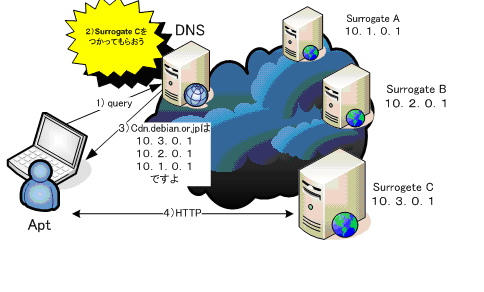
\includegraphics[width=100mm]{image200810/cdn-userviwer.png}
 \end{center}
 \caption{ユーザから見た cdn.debian.or.jp の動作}
 \label{fig:cdn-userviwer}
\end{figure}

サービス時の手順と構成は以下のようになる。(図\ref{fig:cdn-userviwer})

\begin{enumerate}
 \item ユーザがapt-getコマンドを行うとcdn.debian.or.jpをDNSで問い合わせ
       る
 \item cdn.debian.or.jpを管理するDNSはサーバ候補(surrogate)選択する
 \item 選択結果をDNSのリプライとして返す
 \item aptはcdn.debian.or.jpとしてSurrogate Cを使用する。
\end{enumerate}

\subsubsection{構築の方法}

実際にはクライアントDNSは次のように動作している。

\begin{enumerate}
 \item クライアントDNSがcdn.debian.or.jpを検索すると、CNAME
       deb.cdn.araki.netがdebian.or.jpのDNS(BIND)から返答される。
 \item クライアントDNSはdeb.cdn.araki.netを得るためにcdn.araki.netのNSレ
       コードを問い合わせて、ns.cdn.araki.net, plat.debian.or.jp,
       debian.topstudio.co.jp, osdn2.debian.or.jpを得る。
 \item クライアントDNSはいずれかのホストにdeb.cdn.araki.netのAレコードを
       問い合わせて、サロゲートのIPアドレスをdns\_balanceから得る。
 \item クライアントDNSは、ユーザクライアントに3で得た情報を返す。
\end{enumerate}

2を実現するためのAraki.netのBIND設定は次のようになる。

\begin{commandline}
cdn             IN      NS      ns.cdn
                IN      NS      plat.debian.or.jp.
                IN      NS      debian.topstudio.co.jp.
                IN      NS      osdn2.debian.or.jp.
\end{commandline}

\textit{DNS Balance はユーザのIPアドレスと、何らかの方法でサーバをランク
づけした表を元にユーザが接続すべきサイトを指示します。この表は一定時間毎
に読み込み直され、これにより動的な負荷分散が可能です。}

(DNS Balanceの配布ページ\footnote{\url{http://www.dnsbalance.ring.gr.jp}}より)

3を実現するためのdns\_balanceの設定は次のようなサーバをランク付けしたruby
形式のファイルである。
\index{dns balance}
\index{bind}

\begin{commandline}
$addr_db = {
  "default" => {
    "ns.cdn.araki.net" => [
      [[210,157,158,38], 0],
    ],
    "localhost" => [
      [[127,0,0,1], 0],
    ],
 "deb.cdn.araki.net" => [
                [[61,115,118,67], 1000],
                [[133,50,218,117], 10],
                [[202,229,186,27], 20],
                [[133,5,166,3], 10],
                [[130,54,59,159], 10],
                [[210,157,158,38], 9900],
        ], },}
\end{commandline}

この設定ファイルに基づき、ホストIPアドレスの後ろの数字は優先度であり、
1(優先度高)から9999(優先度最低)までの整数で指定する。

\subsubsection{cdn.debian.or.jpのシステムと動作}

CDNシステムが完全に動作しユーザから使用されるためには、システムが完全な
ファイルを提供すること、システムが安定して動作すること、そしてCDNを使っ
た場合に高速に動作していることが求められる。

\subsubsubsection{提供ファイルの完全性}

このために以下二点を満たさねばならない。

\begin{itemize}
 \item 個々のファイルがコンテンツ提供者たるdebファイル配布元と同一である
       こと
 \item apt-get updateの結果取得するファイル群がどのSurrogateでも入手でき
       ること
\end{itemize}

前者については、debはそのファイルのmd5値、sha1値とともに配布され、ユーザ
が使用するaptで確認後に利用されるためCDNを使用した場合でも問題にならない。

後者についてはユーザがapt-get updateを行ったときに接続するSurrogateと
apt-get dist-upgradeを行ったときに接続するSurrogateは同一であるとは限ら
ないため、DNSがSurrogateとして返すサーバが保持するファイルは同一である必
要がある。cdn.debian.or.jpではDebianプロジェクトで一般に行われている方法
と同様に、rsyncプロトコルを用い、pushミラーを行っている(図\ref{fig:cdn-rsync})。そのた
め、cdn.debian.or.jpのサロゲート内で最上流にあるサーバとミラーが同一であ
ることを2分毎にrsyncミラー終了時に作成されるスタンプファイルを確認して、
同一でないサーバはサロゲート候補から一時的に除外している。\index{rsync}

ただし、これはミラーの配送ツリーの管理を行う必要があるため、日本国内のミ
ラーに限定している。

\begin{figure}[htbp]
 \begin{center}
  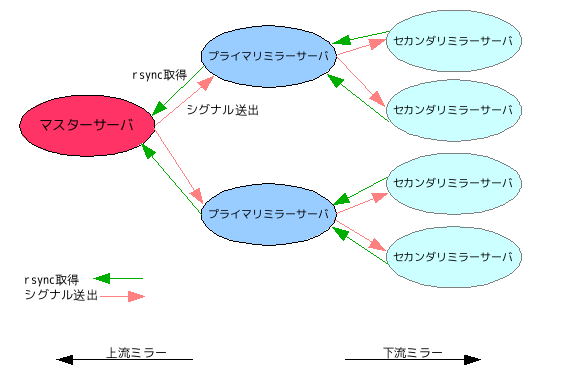
\includegraphics[width=100mm]{image200810/cdn-rsync.png}
 \end{center}
 \caption{Debianサロゲートのrsyncによるミラー}
 \label{fig:cdn-rsync}
\end{figure}

\subsubsubsection{システムの安定動作}

先に述べたように、ユーザはCDNを使用する際にはDNSを最初に使用するため、
DNSの安定運用がカギとなる。そのため、cdn.debian.or.jpを管理するDNSサーバ
はまったく独立に動作するサーバで行っている。

また、サーバの動作を確認は、5秒以内にHTTPのレスポンスを返さないサーバは
サロゲート候補から一時的に除外している。

後述するように、サロゲートの生死確認は2分ごとにdns\_balanceの動作に反映さ
れる。ローカルDNSにキャッシュされる情報とあわせて最悪でも3分以内に動作し
ていないサーバは排除される。

\newpage

\subsubsubsection{高速動作}

cdn.debian.or.jpではDNSで問い合わせされるとサロゲートリストとして複数の
IPアドレスを返す。このIPアドレスはラウンドロビンで選択しているわけではな
く、提供可能なサーバキャパシティやネットワーク速度を考慮し、設定している。

\subsubsection{IPアドレスの位置情報を使用したサーバ選択}

当初はcdn.debian.or.jpとして運用していたものの、その後にglobalに分散する
Debianミラーに対応させた。

globalにCDNを展開する場合には地理的に近いサーバ群からある程度絞込むのが
有効である。現在、GeoIPなど無料でIPと地理情報のマッピング提供者が現れて
おり、debianパッケージになっていることもあり、本システムではMaxmindの
GeoIPを使用している。

Dns\_balanceにはASあるいはネットワークアドレスごとに振り分けるIPアドレス
の指定が可能であるが、

\begin{itemize}
 \item Debianのミラーは国別地域別に制御されていること
 \item 16ビットで指定されるASとAS間の経路の測定が難しい
 \item 個々のネットワーク間の経路を指定するのは現実的でない
\end{itemize}

以上の理由から、dns\_balanceに接続するIPアドレスの国名、大陸名を逆引きし、
その結果をつかって返すAレコードを変更するようにdns\_balanceを拡張してい
る。

大陸別の設定ファイルは次のように、6大陸別である。

\begin{commandline}
yaar@loon3:~/playground/cdn$ ls continent/
AF_deb_cdn_araki_net.rb  EU_deb_cdn_araki_net.rb  OC_deb_cdn_araki_net.rb
AS_deb_cdn_araki_net.rb  NA_deb_cdn_araki_net.rb  SA_deb_cdn_araki_net.rb
\end{commandline}

さらに国別の設定ファイルを置く。

\begin{commandline}
yaar@loon3:~/playground/cdn$ ls country/
FRA_deb_cdn_araki_net.rb  JPN_jp_cdn_araki_net.rb
JPN_deb_cdn_araki_net.rb  KOR_deb_cdn_araki_net.rb
\end{commandline}

これらの設定ファイルをつかって、dns\_balanceが実際に読み込む次のような設
定ファイルを2分ごとに作成している。サーバの生死確認などはこのタイミング
で反映される。

\begin{commandline}
$addr_db = {"default"=>{"localhost"=>[[[127, 0, 0, 1], 0]], "deb.cdn.araki.net"=
>[[[61, 115, 118, 67], 1000], [[61, 206, 119, 174], 20], [[202, 229, 186, 27], 2
0], [[203, 178, 137, 175], 9000], [[210, 157, 158, 38], 9900]], "ns.cdn.araki.ne
t"=>[[[210, 157, 158, 38], 0]], "jp.cdn.araki.net"=>[[[61, 115, 118, 67], 1000],
 [[61, 206, 119, 174], 20], [[202, 229, 186, 27], 20], [[203, 178, 137, 175], 90
00], [[210, 157, 158, 38], 9900]]}, "KOR"=>{"deb.cdn.araki.net"=>[[[143, 248, 23
4, 110], 20]]}, "SA"=>{"deb.cdn.araki.net"=>[]}, "EU"=>{"deb.cdn.araki.net"=>[[[
141, 76, 2, 4], 9000]]}, "AF"=>{"deb.cdn.araki.net"=>[]}, "AS"=>{"deb.cdn.araki.
net"=>[[[61, 115, 118, 67], 1000], [[61, 206, 119, 174], 20], [[202, 229, 186, 2
7], 20], [[203, 178, 137, 175], 9000], [[210, 157, 158, 38], 9900]]}, "JPN"=>{"d
eb.cdn.araki.net"=>[[[61, 115, 118, 67], 1000], [[61, 206, 119, 174], 20], [[202
, 229, 186, 27], 50], [[203, 178, 137, 175], 9000], [[210, 157, 158, 38], 9900]]
, "jp.cdn.araki.net"=>[[[61, 115, 118, 67], 1000], [[61, 206, 119, 174], 20], [[
202, 229, 186, 27], 50], [[203, 178, 137, 175], 9000], [[210, 157, 158, 38], 990
0]]}, "NA"=>{"deb.cdn.araki.net"=>[[[204, 152, 191, 39], 9000], [[128, 30, 2, 36
], 9000], [[35, 9, 37, 225], 9000]]}, "OC"=>{"deb.cdn.araki.net"=>[[[150, 203, 1
64, 37], 9000]]}, "FRA"=>{"deb.cdn.araki.net"=>[[[193, 54, 19, 19], 9000], [[194
, 2, 0, 36], 9000]]}}
\end{commandline}

\newpage

\subsection{使用実績}

以下3ヶ月分のplat.debian.or.jpで動作しているDNSへのアクセス実績を示す。

\begin{itemize}
 \item 2008年7月16日から10月15日までの三ヶ月間の利用実績を解析した。
 \item 本システムではDNSのAまたはAnyに対して返答を戻すことから、それ以外
       のクエリに関しては無効なアクセスとして処理している。
 \item 地域はアクセス元のIPアドレスをGeoIPライブラリから算出している。
 \item 全動作ホストは、plat.debian.or.jp, osdn2.debian.or.jp,
       debian.topstudio.co.jpである。
 \item ユニークホスト数 20554
\end{itemize}

\begin{figure}[!h]
 \begin{tabular}{cc}
  \begin{minipage}{0.5\hsize}
   \begin{center}
    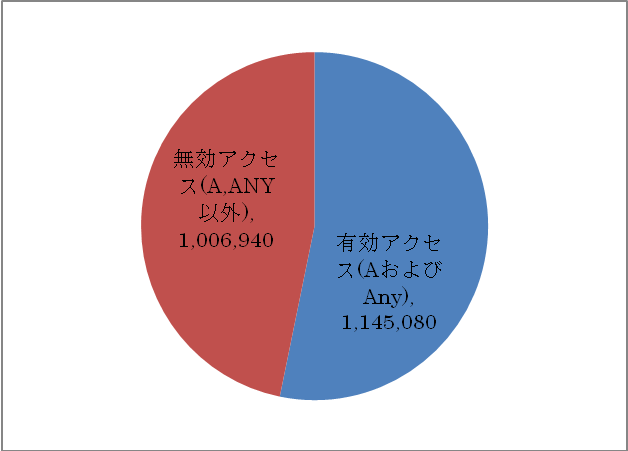
\includegraphics[width=0.7\hsize]{image200810/cdn-access.png}
    \caption{DNSアクセス種別}
    \label{fig:cdn-access}
   \end{center}
  \end{minipage}
  \begin{minipage}{0.5\hsize}
    \begin{center}
     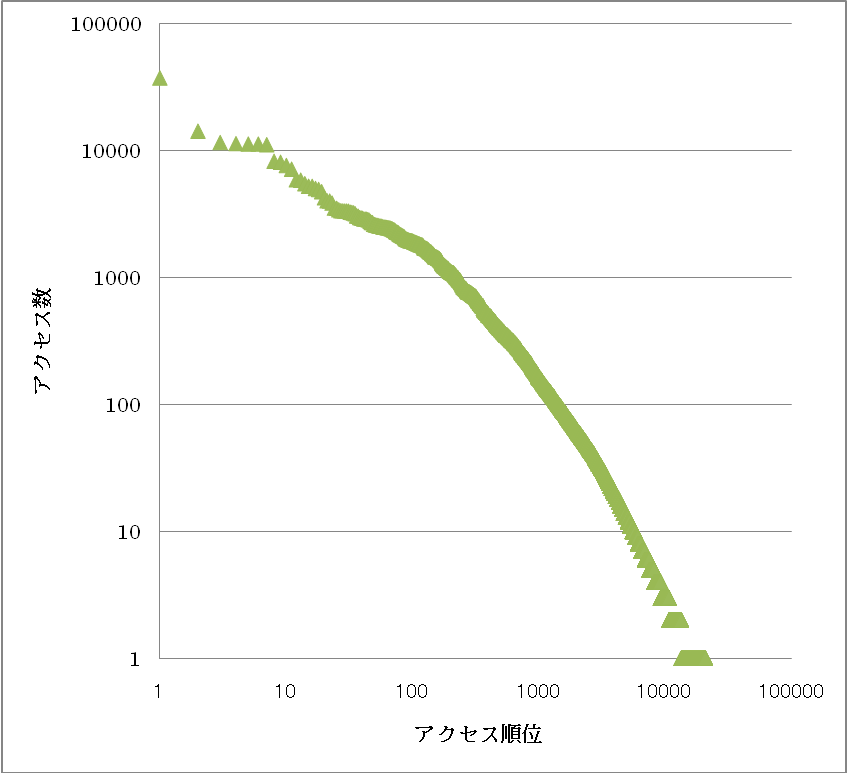
\includegraphics[width=\hsize]{image200810/cdn-access-rank.png}
     \caption{ホスト別アクセス順位とアクセス数}
     \label{fig:cdn-access-rank}
    \end{center}
  \end{minipage}
 \end{tabular}
\end{figure}

ユニークホスト数は20554であるが、その分布は極端に偏っている。

\newpage

\begin{figure}[!h]
 \begin{tabular}{cc}
  \begin{minipage}{0.3\hsize}
   \begin{center}
    \caption{DNSクエリ数上位20カ国}
    \begin{tabular}{|l|r|}
     \hline
     JPN & 808138 \\ \hline
     USA & 87767 \\ \hline
     CAN & 82566 \\ \hline
     KOR & 38596 \\ \hline
     CHIN & 26670 \\ \hline
     FIN & 14558 \\ \hline
     TWIN & 12527 \\ \hline
     IND & 7941 \\ \hline
     IDN & 6463 \\ \hline
     HKG & 5616 \\ \hline
     RUS & 3975 \\ \hline
     SGP & 3656 \\ \hline
     DEU & 2990 \\ \hline
     GBR & 2792 \\ \hline
     AUS & 2635 \\ \hline
     ESP & 2632 \\ \hline
     THA & 2623 \\ \hline
     MYS & 2475 \\ \hline
     PHL & 2359 \\ \hline
     ITA & 2196 \\ \hline
    \end{tabular}
    \label{dnsquerytop20}
   \end{center}
  \end{minipage}
  \begin{minipage}{0.7\hsize}
  \begin{center}
   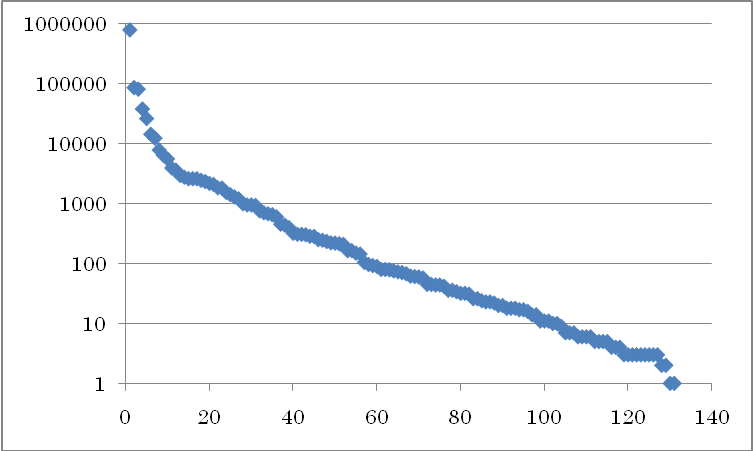
\includegraphics[width=\hsize]{image200810/cdn-query-topcountry.png}
   \caption{DNSクエリ数上位国(横軸)-クエリ数(縦軸)}
   \label{fig:cdn-query-topcountry}
  \end{center}
  \end{minipage}
 \end{tabular}
\end{figure}

なお、国が判定できないのは1552件、率にして0.135\%であった。

\begin{figure}[!h]
 \begin{tabular}{cc}
  \begin{minipage}{0.5\hsize}
   \begin{center}
    \caption{CDN振り分け先実績}
    \begin{tabular}{|l|r|l|}
     \hline
     地域 & \multicolumn{1}{l|}{アクセス数} &  \\ \hline
     アジア & 570137 &  \\ \hline
     アジア(日本と韓国除く) & \multicolumn{1}{l|}{} & \multicolumn{1}{r|}{55539} \\ \hline
     日本 & \multicolumn{1}{l|}{} & \multicolumn{1}{r|}{509367} \\ \hline
     韓国 & \multicolumn{1}{l|}{} & \multicolumn{1}{r|}{5231} \\ \hline
     ヨーロッパ & 16804 &  \\ \hline
     ヨーロッパ(フランス除く) & \multicolumn{1}{l|}{} & \multicolumn{1}{r|}{15154} \\ \hline
     フランス & \multicolumn{1}{l|}{} & \multicolumn{1}{r|}{1650} \\ \hline
     北米 & 142207 &  \\ \hline
     オセアニア & 10766 &  \\ \hline
     アフリカ & 160 &  \\ \hline
     その他 & 404996 &  \\ \hline
     総有効アクセス数 & 1145070 &  \\ \hline
    \end{tabular}
    \label{dnsquery}
   \end{center}
  \end{minipage}
  \begin{minipage}{0.5\hsize}
   \begin{center}
    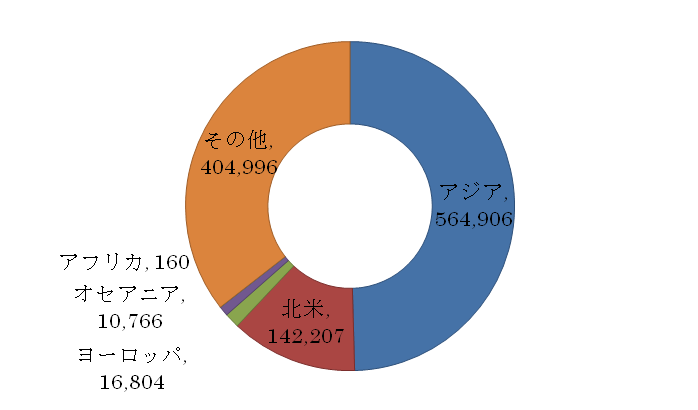
\includegraphics[width=0.9\hsize]{image200810/cdn-area-world.png}
    \caption{地域別振り分け実績}
    \label{fig:cdn-area-world}
   \end{center}
  \end{minipage}
 \end{tabular}
\end{figure}

\newpage

\begin{figure}[!h]
 \begin{tabular}{cc}
  \begin{minipage}{0.3\hsize}
   \begin{center}
    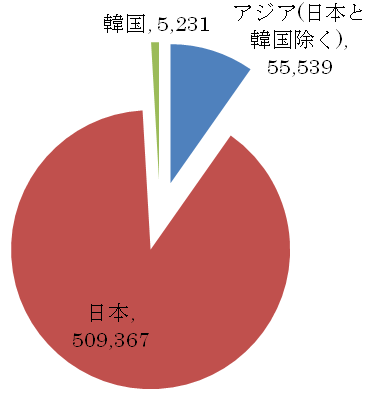
\includegraphics[width=0.8\hsize]{image200810/cdn-area-asia.png}
    \caption{アジア地域の振り分け実績}
    \label{fig:cdn-area-asia}
   \end{center}
  \end{minipage}
  \begin{minipage}{0.7\hsize}
   \begin{center}
    \caption{日本での振り分け実績}
    \begin{tabular}{|l|l|r|}
     \hline
     \textbf{ホスト名} & \textbf{IP} & \multicolumn{1}{l|}{\textbf{振り分け数}} \\ \hline
     runner.oyu-net.jp. & 61.206.119.174 & 690596 \\ \hline
     dwarf.topstudio.co.jp. & 202.229.186.27 & 660091 \\ \hline
     hanzubin.st.wakwak.ne.jp & 61.115.118.67 & 649512 \\ \hline
     studenno.kugi.kyoto-u.ac.jp. & 130.54.59.159 & 599550 \\ \hline
     dennou-q.geo.kyushu-u.ac.jp & 133.5.166.3 & 468730 \\ \hline
     frost.nemui.org. & 218.219.152.77 & 445589 \\ \hline
     dennou-h.ep.sci.hokudai.ac.jp. & 133.87.45.30 & 379888 \\ \hline
     ftp.nara.wide.ad.jp & 203.178.137.175 & 58825 \\ \hline
     plat.debian.or.jp & 210.157.158.38 & 6095 \\ \hline
    \end{tabular} 
   \end{center}
   \label{dnsjapansymmetry}
  \end{minipage}
 \end{tabular}
\end{figure}

% \begin{figure}[!h]
%  \begin{center}
%   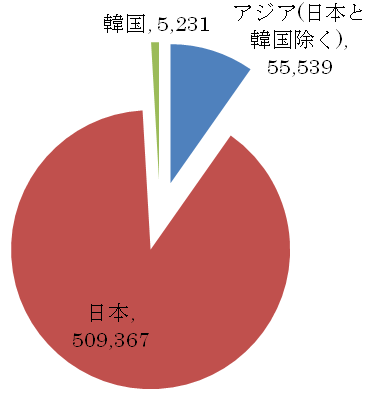
\includegraphics[width=100mm]{image200810/cdn-area-asia.png}
%  \end{center}
%  \caption{アジア地域の振り分け実績}
%  \label{fig:cdn-area-asia}
% \end{figure}

アジア地域向けのサーバおよび韓国地域向けのサーバは日本向けのサーバ群設定
と全く同一のものを設定している。

% \begin{table}[!h]
%   \caption{日本での振り分け実績}
%  \begin{center}
%   \begin{tabular}{|l|l|r|}
%    \hline
%    \textbf{ホスト名} & \textbf{IP} & \multicolumn{1}{l|}{\textbf{振り分け数}} \\ \hline
%    runner.oyu-net.jp. & 61.206.119.174 & 690596 \\ \hline
%    dwarf.topstudio.co.jp. & 202.229.186.27 & 660091 \\ \hline
%    hanzubin.st.wakwak.ne.jp & 61.115.118.67 & 649512 \\ \hline
%    studenno.kugi.kyoto-u.ac.jp. & 130.54.59.159 & 599550 \\ \hline
%    dennou-q.geo.kyushu-u.ac.jp & 133.5.166.3 & 468730 \\ \hline
%    frost.nemui.org. & 218.219.152.77 & 445589 \\ \hline
%    dennou-h.ep.sci.hokudai.ac.jp. & 133.87.45.30 & 379888 \\ \hline
%    ftp.nara.wide.ad.jp & 203.178.137.175 & 58825 \\ \hline
%    plat.debian.or.jp & 210.157.158.38 & 6095 \\ \hline
%   \end{tabular} 
%  \end{center}
%  \label{dnsjapansymmetry}
% \end{table}

日本での振り分け実績は、設定した頻度情報をほぼ正確に反映しており、プログ
ラムの動作および、期間中の各サロゲートに大きな障害がなかったことを示して
いる。

\subsection{関連研究とディスカッション}

\url{http://prisms.cs.umass.edu/~kevinfu/papers/secureupdates-hotsec06.pdf}
でのサーベイ結果のように、パッケージ配布にはいくつかの方法と危険性が指摘
されている。このサーベイ結果で指摘されるように、Debianでは個々のファイル
ごとに\texttt{sha-1}および\texttt{MD5},\texttt{SHA-256}のハッシュ値を配布している。

加えて、本システムの日本での運用においては、マスターサーバからサロゲート
へのファイル同期時に配送ツリーの確認とファイルの一致を確認しており、障害
時の排除機能を有するため、単なるファイルのミラーリング以上の安全性は確保
されている。

openSUSE における配送
(mirrorbrain, \url{http://en.opensuse.org/Build_Service/Redirector} )
はsourceforgeをはじめ多くのCDNで採用している方法である。クライアントへの
サロゲート決定の方法はGeoIPを使用しており、本システムと同等のものである。

ただし、Debianのaptシステムの制限により、本システムではHTTPリダイレクト
ではなく、DNSを使用している。

また、mirrorbrainではサロゲートへの配送の確認は行っていないものと思われ
る。

aptのP2P対応も有力な配布手段である。apt-p2p
\footnote{\url{http://www.camrdale.org/apt-p2p/}}
により、aptのP2P対応が進められている。有力な候補である。ただし、Kashimir
プロトコルをクライアントで直接使うものであり、ネットワーク利用ポリシーと
の競合やinstall時に利用できない点、取得希望ファイルが入手できない場合に
HTTPにフォールバックするため速度に問題があり、今後検証すべき問題も多い。

サロゲートが正しく動作しているのか、その能力に応じたサロゲート使用ができ
ているかどうかは、分散したファイルサーバからのファイル入手において重要な
要素である。この組み合わせを考えると、表\ref{health check}のように分類される。本システ
ムでは、サーバやサーバとクライアント間のネットワークの実測を行わないこと、
ここのサロゲートの運用は独立して行うことでサロゲートへ特別なプログラムを
必要としないことで、コストの劇的な削減を可能としている。

\begin{table}[htbp]
\caption{}
\begin{tabular}{|l|l|l|}
\hline
 & 申告ベースの能力 & 動的測定・実績ベースの能力 \\ \hline
申告ベースのヘルスチェック & Debianミラーサーバリスト & Debianミラーの口コミ・トライアンドエラー \\ \hline
動的測定・実績ベースのヘルスチェック & 本システム & 理想的なシステムだがコスト大
商用CDNなど \\ \hline
\end{tabular}
\label{health check}
\end{table}

\subsection{課題と将来の展望}

ここまで説明してきた、cdn.debian.or.jpの動作には改善すべき点が多数存在する。改善の展望としていくつか挙げる。

\subsubsection{アクセス実績あるいはローカルポリシーに基いたCDN配置}

アクセス実績によると、日本、米国、カナダ、韓国、中国、フィンランド、台湾、
インド、インドネシア、ホンコン、ロシアと続く。現状では、大陸毎に設定され
たサロゲートは存在するものの、日本、韓国、アメリカを除けば国毎に設定さ
れたサロゲートは存在しない。

このアクセス実績にもとづき、これらの国内のミラーを生かした設定を近い将来
行いたい。

\subsubsubsection{apt-getコマンドのHTTP REDIRECT}

apt-getコマンドはHTTP REDIRECTに対応していない。

そのため、前述したようにmirrorbrainなどのCDNは使用することができない。

HTTP REDIRECTは、いったんHTTP GETなどで接続してきたクライアントに対して、
新たにそのリソースが存在するURLを通知するものである。この仕組みをうまく
つかったCDNとして、Coral Content Distribution Network (Coral CDN)がある。
Coral CDNはサロゲート間でP2Pによるファイル配置し、そのインターフェースと
して、HTTPを使用し、しかも使用にはインターネットから取得可能なファイルで
あれば制限をかけていない。さらに、Apacheを使った一時配布サーバではHTTP
REDIRECTをつかってCoral CDNに誘導することも推奨されている。ただし、現状
で、Coral CDNを使うために、

\begin{commandline}
deb http://cdn.debian.or.jp.nyud.net:8090/debian/ stable main contrib non-free
\end{commandline}

を指定することも可能だが、少なくとも日本においてはCoral CDNを担うサロゲー
トが存在しないこともあって非常に低速である。ただし韓国や中国では広くつか
われており、将来の拡張に使用したい。

\subsubsubsection{マスターサーバからサロゲートへのミラーリング方法}

本システムでは既存のrsyncによるミラーリング手法には手をつけていない。行っ
たのはrsyncをつかってタイムスタンプを確認し、サロゲートのヘルスチェック
のひとつに使用したのみである。debianにおけるrsyncの使い方現状のミラーリ
ングに由来する問題は

\begin{enumerate}
 \item master.debian.orgから末端までのあいだは冗長化されていない
 \item rsyncはディレクトリの同期を取る方法であり、ファイルの転送に必ずし
       も適していない。debのように依存関係を記述したメタデータを含むファ
       イルであれば、ファイル毎のpushであっても配送に問題はない
 \item 配送がユニキャストである
 \item 利用頻度や重要度にかかわらず同様の配送を行っている 
\end{enumerate}

等さまざまである。

Debianが潤沢なネットワーク環境と強力なCPUを要するホストでない場合でもミ
ラーリングないしサロゲートからのファイル入手を可能とするFLUTEなどの配送
手法が必要になろう。

\subsection{おわりに}

いつでも必要なソフトウェアやコンテンツを安価に入手する手段としてCDNはこ
れからも様々な発展を続けると考える。Debianはdebの安定入手手段の有無がシ
ステムの信頼性を左右するシステムであり、CDNの広範な活用が今後ますます求
められるようになると考える。

本システムの導入により、サロゲート個々の安定性がクライアントに直接影響す
ることはかなり抑えることができるが、より確実なパッケージ入手のために、信
頼性が高く安定動作しているサロゲートの増加をDebianプロジェクトでは引き続
き求めている。

% 200811
% KOF のため資料なし


\clearpage

%%%  月例アップデート

%===========================================================%
\begin{getsureiupdate}{月例 Debian GNU/kFreeBSD}{大浦 真}
\index{kFreeBSD}
今月は Debian GNU/kFreeBSD のインストーラについて見てみましょう。

現在、Debian GNU/kFreeBSD には、Debian で使われている
Debian Installer (d-i) は用意されていません。
d-i を移植する計画はあるようですが、今はその代わりに、
FreeBSD のインストーラを改造したものが使われています。
アーキテクチャとしては、i386 向けと amd64 向けが用意されていて、
最新版は 2008年2月18日にリリースされたものです。

このインストーラを使って実機や QEMU などの仮想マシンにインストールする
ことができますが、このインストーラは、FreeBSD のインストーラを
必要最低限の部分だけ改造したものです。
ですので、kFreeBSD のインストールには、注意すべき点がいくつかあります。
まず、インストールの手順が FreeBSD のインストール方法とも
だいぶ異なっているという点があります。
これは、この稿の末尾に URL を挙げた Install Guide に手順が記載されていますが、
普通の FreeBSD のインストーラのつもりでインストールを行うと
うまくいかないので注意が必要です。
また、インストーラはベースシステムのインストールしか行わないので、
root のパスワードの設定、一般ユーザの作成、ネットワークの設定、
ftp.debian-ports.org のアーカイブキーの取得などの
基本的な設定は全て手動で行う必要があります。
ただ、Install Guide に従いさえすれば、比較的簡単にインストールを
完了することができますし、使い慣れた Debian システムなので、
設定もしやすいでしょう
\end{getsureiupdate}
%===========================================================%

%===========================================================%
\begin{getsureiupdate}{月例 Nexenta Operating System}{上川 純一}
\index{Nexenta}
先月につづいてNexentaをいじって見たのでお伝えします。

今月は cowdancer をビルドするところまで、です。\index{cowdancer}
まず、ソースコードをビルドしてみましょう。
警告も大量に出るのですが、とりあえずは絶望しないためにエラーを眺めてみましょう。

\begin{commandline}
$ make 
gcc -O2 -Wall -o cow-shell cow-shell.o ilistcreate.o
cow-shell.o: In function
 `main':/export/home/dancer/cowdancer-0.36/cow-shell.c:26: 
undefined reference to `asprintf' 
:/export/home/dancer/cowdancer-0.36/cow-shell.c:60: undefined
reference to `canonicalize_file_name' 
collect2: ld returned 1 exit status
make: *** [cow-shell] Error 1
dancer@vm1:~/cowdancer-0.36$ 
\end{commandline}

まず、canonicalize\_{}file\_{}name, asprintf, dlvsym などの関数が無いと
 いう旨のエラーが出ています。これらがどうやらGNU/Linux(glibc)で提供され
 ている拡張で、そのままでは Solaris 上では動かなさそうですね。

ということで、GNU拡張をどう処理するのかに悩みます:

\begin{itemize}
 \item dlvsym: ダイナミックライブラリの関数をバージョン指定で読み込む。
       あきらめて dlsym をそのまま使えば良いんじゃないか?
 \item canonicalize\_{}file\_{}name: 
       realpath を代わりに使えばよいんじゃないか?
 \item asprintf: asprintf のバッファを確保してくれるバージョンなので、バッ
       ファを最初から用意して sprintf を代替として利用すればよいんじゃな
       いか?
\end{itemize}
といったところまでいじったところでまた来月。

\end{getsureiupdate}
%===========================================================%


%===========================================================%
\begin{getsureiupdate}{月例 Debian GNU/Linux eeepc port}{岩松 信洋}
\index{eeePC}
不定期連載の Debian GNU/Linux eeepc port です。
先月、会長から押し付けられた eeepc に Debian を SDHC カードにインストールしてみました。
debian-eeepc project によって、インストーラーが用意されており、
USBメモリにコピーして利用できるようになっています。インストール自体は Debian のインストーラと同じです
が、eeepc に搭載されている無線LANのドライバが利用できるようになっています。
インストールはさくさく進むと思っていたのですが、どうも SDHC への書き込みが遅いようです。
base をインストールするのに 2時間もかかりました。
ネットワークを使ったパッケージの取得までは順調なのですが、パッケージのインストール
でかなり時間がかかっています。また、インストールした後のパッケージインストールにも
時間がかかります。
調べたところ、Linux カーネルのプリエンプションオプションの設定が問題だということがわかりました。
変更したカーネルを作ったところサクサク動いています。
今度は、カーネルの設定を変更したインストーラを作って試してみようと思います。
\end{getsureiupdate}
%===========================================================%



%===========================================================%
\begin{getsureiupdate}{月例 Nexenta Operating System}{上川 純一}
\index{Nexenta}

前回は実用的なアプリケーションをビルドするまでに至りませんでした。
そこで、今回は dlsym を使って自由自在にライブラリをロードできるようにしてみるところから
 まずやってみましょう。
dlsymでロードできる最低限の共有ライブラリを作成するところから始めてみま
す。

まず、関数一つだけを定義したCのファイルから最低限の共有ライブラリを作成
 して、それを実行するだけのプログラムと、dlopen経由で利用するプログラ
 ムを作成してみました。

\begin{commandline}
// a.c : サンプルの共有ライブラリのコード
#include <stdio.h>

void func1 (int i)
{
  printf(" hello world %i\n", i);
}
\end{commandline}

\begin{commandline}
// use.c: 通常の共有ライブラリ利用
#include <stdio.h>

void func1 (int i);

main()
{
  func1(1);
}
\end{commandline}

\begin{commandline}
// dlopen.c: dlopenでのバイナリ利用
#include <dlfcn.h>
static int (*myfunc1)(int i) = NULL;
int main()
{
  void* h=dlopen("./liba.so", RTLD_NOW);
  
  myfunc1=dlsym(h, "func1");
  
  myfunc1(10);
  
  return 0;
}
\end{commandline}

これらをコンパイル、リンクしてみて、動作を確認してみました。
どうやらLinuxとあまりかわらないようです。

\begin{commandline}
 + gcc -shared a.c -o liba.so
 + gcc use.c ./liba.so -o use
 + ./use
 hello world 1
 + gcc dlopen.c -o dlopen
 + ./dlopen
 hello world 10
\end{commandline}

ただし、これだけだとバージョンシンボルを利用した場合にdlsym ではどのバー
 ジョンを利用するのかが指定できないような雰囲気がただよっています。
というところまで確認したところで今月も力尽きました。
また来月続きをながめてみましょう。
もしかするとバージョンシンボルの作成とその利用をするかもしれません。

\end{getsureiupdate}
%===========================================================%

% quiz
%% tokyoquiz-200807
%%% trivia quiz
\dancersection{Debian Trivia Quiz}{上川 純一}

ところで、みなさん Debian 関連の話題においついていますか?Debian関連の話
題はメーリングリストをよんでいると追跡できます。ただよんでいるだけではは
りあいがないので、理解度のテストをします。特に一人だけでは意味がわからな
いところもあるかも知れません。みんなで一緒に読んでみましょう。


\begin{multicols}{2}
 \subsection{第42回勉強会}
% 出題範囲: http://lists.debian.org/debian-devel-announce/2008/06/msg00004.html 〜 http://lists.debian.org/debian-devel-announce/2008/07/msg00004.html
第42回勉強会の出題範囲は\url{debian-devel-announce@lists.debian.org} に投稿された
内容と Debian Project News からです。

 \santaku
 {Perl 5.10のバグでどのような問題が発生した?}
 {RubyとPythonで書かれたアプリケーションやライブラリがインストールできない}
 {インストールされたファイルのパーミッションが0777になる}
 {特定の名前のファイルがインストールできない}
 {B}
{File::Path::rmtreeがツリー削除前にパーミッションを0777にし、それがsymlinkのリンク元にも伝播するようになっていたのが原因。postinstで呼び出されるdebsignがツリーのsymlinkを作成してハッシュを計算した後、この関数を使ってsymlinkを削除しているので、インストール後にファイルのパーミッションが書き換えられる問題に発展した}

 \santaku
 {Debianプロジェクト内のチームに関する調査で判明した「予想外のチーム」でないものは?}
 {実際に動いているのは1人だけというチーム}
 {誰が作業するか毎回じゃんけんで決めているチーム}
 {お願いやありがとうではなく脅迫で動いているチーム}
 {B}
{調査はDPLのSteve McIntyreが行っている}
 
 \santaku
 {wxwidgets2.8がアップロードされたが、長いことwxwidgets2.6の時代が続いていた。その理由は?}
 {パッケージメンテナが保守的で、2.8の使用に対して非積極的だった}
 {アップロードしたところでどうせ誰も使ってくれないとパッケージメンテナが思った}
 {パッケージメンテナが多忙で作業時間がとれなかった}
 {A}
{lennyでは2.6をデフォルトとし、2.6で動かないものだけ2.8を使ってほしい、とのこと}

 \santaku
 {Frans Popの辞任によって、新たな執筆者が求められるようになったものとは?}
 {リリースノート}
 {Debian Project Blog}
 {DEB NOTE}% 名前が書かれた開発者を強制的にコミュニティから追い出すノート
 {A}
 {Debian Project公式のblog}
 
 %\subsection{Debian Project News 2008年05号}
 %\url{http://www.debian.org/News/weekly/2008/05/}
 %にある6月23日版です。
 
 \santaku
 {debian/rulesのget-orig-sourceターゲットは何を記述するためのものか?}
 {「オリジ○弁当」で弁当にソースをつけてもらう方法}
 {upstreamからネットワーク経由でソースコードを取得して現在のソースコードと置き換える方法}
 {upstreamからネットワーク経由で最新の.orig.tar.gzファイルを取得する方法}
 {C}% あまり書かれることのないターゲットだが、skkdicではCVS経由で取得するよう設定している
 {}

 \santaku
 {リリースゴールに関するPeter Eisentrautの意見は?}
 {リリースゴールなんて所詮一部の開発者の楽しみに過ぎない}
 {Debianの機能の実装に関するリリースゴールはリリース後にポリシーへと変えるべきだ}
 {リリースなんて飾りです。偉い人にはそれがわからんのですよ}
 {B}
 {}
 
 \santaku
 {William Pitcockが削除を提案したブートローダパッケージは?}
 {grub}
 {lilo}
 {yaboot}
 {B}% 簡単には直せないgraveなバグがある
 {}
 
 \santaku
 {Debian weatherとはどんなサービスか?}
 {特定アーキテクチャのアーカイブの状態を要約して表示する}% その表示に天気の記号を使用している
 {Debian関連ホストが置かれている世界各地の天気を表示する}% worldwideで働いているという意識を高める
 {メーリングリストの流量から世界各地の天気を推測して表示する}% この地域からのメールが多いからこの地域は雨だな、とか
 {A}
 {}
 
 %\subsection{Debian Project News 2008年06号}
 %\url{http://www.debian.org/News/weekly/2008/06/}
 %にある7月7日版です。
 
 \santaku
 {Debian 15周年はいつか?}
 {次回の東京エリアDebian勉強会開催予定日である8月16日}
 {本日7月19日}
 {泣く子も黙る7月9日}
 {A}
 {}
 
 \santaku
 {Debianのメニュー (.menuファイル) とデスクトップ環境のメニュー (.desktopファイル) に関する議論はどのような結論に落ち着いたか?}
 {freedesktop.orgの.desktopファイルをDebianに合うよう拡張して使っていこう}
 {freedesktop.orgの.desktopファイルには不便な点があるので、働きかけて修正してもらおう}
 {freedesktop.orgの.desktopファイルは使えないのでDebianの.menuファイルを使わせよう}
 {A}% .desktopメニューはユーザビリティを目的とするもので単一階層 (サブカテゴリなし) なのに対し、Debianのメニューは完全性を目的とするもので階層を深く掘っている。ちなみに.menuに比べて.desktopのほうがいいという人はかなり多そう
 {}
 
 \santaku
 {6月末に初めて誕生したDebian開発者同士の夫婦とは?}
 {Junichi UekawaとKenshi Muto}
 {Meike ReichleとAlexander Schmehl}
 {Debra MurdockとIan Murdock}% 実はDebraさんがDDになり今更ながら結婚、とか
 {B}
 {}
 
 \santaku
 {結婚した二人について述べた以下の事項のうち、正しいものは?}
 {最初の贈り物: DebConf5の土産}% 具体的にはDebConf5のTシャツとフィンランドのチョコレート
 {秘密の愛の交換手段: wiki.debian.org}% planet.d.oで交換していたら誰かに書き換えられた
 {婚約の公式発表手段: lists.debian.org}% planet.d.oで発表したら名前を書き換えられた
 {A}
 {}


%% tokyo-quiz200809
 \subsection{第44回勉強会}
 第44回勉強会の出題範囲は\url{debian-devel-announce@lists.debian.org}への投稿内容と Debian Project Newsからです。
 
 \santaku
 {今年も Debconf が開催されました。どこで開催されたでしょうか。}
 {中国}
 {アルゼンチン}
 {スペイン}
 {B}
 {中国は 北京でオリンピック、スペインは次回、今回はアルゼンチン}
 
 \santaku
 {ギブアップ宣言をした Debian サブプロジェクト/チームは何でしょうか}
 {The Debian Live project}
 {The Debian EEEPC team}
 {The Debian Jr. project}
 {C}
 {マンパワーが足りないのと進展がほとんどないため}

 \santaku
 {Lenny frozen が宣言されたのはいつでしょうか?}
 {2008/07/26}
 {2008/07/27}
 {2008/07/28}
 {B}
 {HEによってフリーズ宣言}
 
 \santaku
 {Andreas Schuldei が立ち上げた新しいチームは何でしょうか。}
 {Debian マーケティング チーム}
 {Debian Dream チーム}
 {Debian Chrome チーム}
 {A}
 {}

 \santaku
 {Debian GNU/Linux 4.0 のアップデート版が出ましたが、何と呼ばれているでしょうか。}
 {etch and lenny}
 {etch with you}
 {etch and a half}
 {C}
 {}

 \santaku
 {リリースに向けての作業が佳境に入っています。このような作業の中、lennyの次のバージョンとなるリリースのコードネームが決まりました。何でしょうか。}
 {3つ目エイリアン squeeze}% 3つ目エイリアン
 {言葉遊びのオモチャ spell}%言葉遊びのオモチャ
 {重量挙げ選手のアクションフィギュア rocky}%重量挙げ選手のアクションフィギュア
 {A}
 {}


%% tokyoquiz-200810
%% None
%% tokyoquiz-200811
\subsection{第46回勉強会}
 第46回勉強会の出題範囲は\url{debian-devel-announce@lists.debian.org}への投稿内容と
 Debian Project News からです。

 \santaku
 {BTS 500000番はどんなバグ報告だったでしょうか}
 {SPAMだった}
 {cdbs に defoma 対応させるためのパッチ}
 {Lenny リリースが遅れているというバグ報告}
 {B}
 {}

 \santaku
 {10月25日から30日まで行われた BTS の景品は何でしょう?}
 {DPLからのキス}
 {次回のDebconf無料チケット}
 {おいしいクッキー}
 {C}
 {}
 
 \santaku
 {screenshots.debian.net は何をまとめたサイトでしょうか?}
 {デスクトップのスクリーンショット}
 {ソフトウェアのスクリーンショット}
 {Debian Developerのプライベート写真集}
 {B}
 {}

 \santaku
 {Joerg Jaspertがプロポーザルを出したDebian membershipとは?}
 {「Debian開発者」の現在の定義を変えるための提案}
 {Debian開発者の家族に関する提案}
 {Debianからforkしたディストリに関する提案}
 {A}
 {}
 % http://lists.debian.org/debian-devel-announce/2008/10/msg00005.html

 \santaku
 {Debian Installer team から出たアナウンスは何でしょう?}
 {ごっめーん!インストーラー遅れちゃった。}
 {Debian Installer lenny RC1 出たよ}
 {RC1 は飛ばして リリースする予定です。}
 {A}
 {}
\end{multicols}
%% quiz 終わり

\dancersection{Debian Trivia Quiz 問題回答}{上川 純一}

\begin{multicols}{2}
 Debian Trivia Quiz の問題回答です。
 あなたは何問わかりましたか?
 \\
 %回答はdebianmeetingresume2008-fuyu.jqzというファイルに生成されるので、
 %それを手動でコピペして使う。
 % ここからコピペ
 % FIXME 問題が全部はいったらコピペすること
 %(progn (next-line 1)(insert-file "debianmeetingresume2008-fuyu.jqz") )
1. B\\
2. B\\
3. A\\
4. A\\
5. C\\
6. B\\
7. B\\
8. A\\
9. A\\
10. A\\
11. B\\
12. A\\
13. B\\
14. C\\
15. B\\
16. A\\
17. C\\
18. A\\
19. B\\
20. C\\
21. B\\
22. A\\
23. A\\


\end{multicols}


\printindex

\cleartooddpage

\thispagestyle{empty} 
{
\large
\begin{itembox}{\bf 『あんどきゅめんてっど でびあん』について}
本書は、東京および関西周辺で毎月行なわれている『東京エリア Debian 勉強会』および
『関西エリア Debian 勉強会』で
使用された資料・小ネタ・必殺技などを一冊にまとめたものです。
収録範囲は東京エリアは勉強会第41回から第46回、関西エリアは
第14回から第19回まで。
% FIXME: 回数を修正すること。
内容は無保証、つっこみなどがあれば勉強会にて。
\end{itembox}
}

\vspace*{15cm}
{\color{dancerlightblue}\rule{\hsize}{1mm}}
\vspace{2mm}

\includegraphics[width=2cm]{image200502/openlogo-nd.eps}
\noindent \Large \bf あんどきゅめんてっど でびあん 2008年冬号\\ \\
% FIXME 開催日がわかったら更新すること
\noindent \normalfont 2008年12月29日 \hspace{5mm}  初版第1刷発行\\
\noindent \normalfont 東京エリア Debian 勉強会/関西エリア Debian 勉強会 (編集・印刷・発行)\\
{\color{dancerdarkblue}\rule{\hsize}{1mm}}

\end{document}
